% !LW recipe = AM (XeLaTeX)
\PassOptionsToPackage{no-math}{fontspec}
\documentclass[11pt,UTF8,scheme=plain,fontset=fandol,linespread=1.3]{ctexart}
\usepackage[skip=0.55\baselineskip plus 2pt]{parskip}
\usepackage{amsmath, amsthm, amsfonts, amssymb, bm}
\usepackage{dsfont}
\usepackage{mathrsfs}
\usepackage{newtxtext}
\newfontfamily\blocktitleface{texgyrepagella}[
  Extension=.otf,
  UprightFont=*-regular,
  BoldFont=*-bold,
  ItalicFont=*-italic,
  BoldItalicFont=*-bolditalic
]
\usepackage[backend=bibtex,style=numeric,sorting=none]{biblatex}

\usepackage[bookmarks=true, unicode, colorlinks, citecolor=blue, linkcolor=black]{hyperref}
%bookmarks=true: enable PDF bookmarks for navigation.
%colorlinks: colored link text instead of boxed links.
%citecolor=blue: citation link color.
%linkcolor=black: ordinary link color (e.g. TOC).
\usepackage{geometry}
\usepackage[dvipsnames,svgnames]{xcolor}
\usepackage[strict]{changepage} % adjustwidth environment
\usepackage{framed}
\usepackage[most]{tcolorbox}
\usepackage{float}
\usepackage{pifont} % circled numbers / dingbats
\usepackage{subcaption}
\usepackage{booktabs}
\usepackage{url}
% Restart figure numbering each section.
\numberwithin{figure}{section}

%%% Fonts: XeLaTeX + ctex. scheme=plain keeps English structural names.
% \songti 宋体, \heiti 黑体, \fangsong 仿宋, \kaishu 楷书。

\everymath{\displaystyle}% global display-style math in inline math
\usepackage{etoolbox}

% Math shortcuts + shared notation / algorithm helpers (from writing preamble).
%% ===================================================================
%%  NOTATION AND NAMING CONVENTIONS
%%
%%  Two bold-math font families, separated by semantic role
%%  (all \v* and \m* macros are \bm{...}, defined in math_commands.tex):
%%
%%  1. Vectors (\v... macros)
%%     \vu, \vu_0    : generic optimization variable / initial point
%%     \vx, \vy, \vz : sequence variables (e.g. Nesterov triples)
%%     \vg           : gradient / surrogate gradient
%%     \vb           : RHS / data vector
%%     \vzero, \vone : zero / all-ones vectors
%%     \vxi, \vnu, \vbeta, \vtheta, \vlambda, \vmu : bold Greek vectors
%%
%%  2. Matrices (\m... macros, uppercase)
%%     \mA, \mB, \mC : design / system matrices
%%     \mI           : identity
%%     \mX, \mY, ... : general bold matrices
%%
%%  3. Common operators (math_commands.tex + macros.tex)
%%     \R, \E, \Ls, \argmax, \argmin, \sign, \Tr, \prox, \Lip, \dom, \dist, \rank
%%     \abs{...}, \norm{...}   (mathtools paired delimiters; \abs* / \norm* auto-size)
%%     \ip{x}{y}               inner product
%%     \oracle                 matrix--vector oracle
%%
%%  4. Theorem / note environments (main.tex)
%%     Standard: definition, theorem, lemma, proposition, corollary,
%%               remark, example, proof, solution
%%     Styled:   defblock, thmblock, axiomblock, lemmablock, propositionblock, colblock,
%%               exampleblock, exerciseblock, remarkblock
%%
%%  Project-specific experiment labels or paper-only macros belong in a
%%  local file (e.g. paper_macros.tex), not in this shared preamble.
%% ===================================================================

% Official optional notation definitions.
%%%%% MATH SHORTCUTS %%%%%
% General vector / matrix / operator macros for research notes.
% Loaded after amsmath + bm. Does not redefine theorem environments.
%
% Font families (semantic role; both render as bold math via \bm):
%   1. Vectors   \v...   e.g. \vx, \vy, \vz, \vzero, \vone
%   2. Matrices  \m...   e.g. \mA, \mB, \mI  (uppercase)
%   3. Tensors   \t...   e.g. \tA
%   4. Calligraphic / sets: \gA (graph-like), \sR (blackboard sets)
%
% Prefer amsmath \eqref{...} for parenthesized equation references.

% Mark sections of captions for referring to divisions of figures
\newcommand{\figleft}{{\em (Left)}}
\newcommand{\figcenter}{{\em (Center)}}
\newcommand{\figright}{{\em (Right)}}
\newcommand{\figtop}{{\em (Top)}}
\newcommand{\figbottom}{{\em (Bottom)}}
\newcommand{\captiona}{{\em (a)}}
\newcommand{\captionb}{{\em (b)}}
\newcommand{\captionc}{{\em (c)}}
\newcommand{\captiond}{{\em (d)}}

% Highlight a newly defined term
\newcommand{\newterm}[1]{{\bf #1}}

% Figure / section / algorithm references
\def\figref#1{figure~\ref{#1}}
\def\Figref#1{Figure~\ref{#1}}
\def\twofigref#1#2{figures \ref{#1} and \ref{#2}}
\def\quadfigref#1#2#3#4{figures \ref{#1}, \ref{#2}, \ref{#3} and \ref{#4}}
\def\secref#1{section~\ref{#1}}
\def\Secref#1{Section~\ref{#1}}
\def\twosecrefs#1#2{sections \ref{#1} and \ref{#2}}
\def\secrefs#1#2#3{sections \ref{#1}, \ref{#2} and \ref{#3}}
\def\Eqref#1{Equation~\ref{#1}}
\def\plaineqref#1{\ref{#1}}
\def\chapref#1{chapter~\ref{#1}}
\def\Chapref#1{Chapter~\ref{#1}}
\def\rangechapref#1#2{chapters\ref{#1}--\ref{#2}}
\def\algref#1{algorithm~\ref{#1}}
\def\Algref#1{Algorithm~\ref{#1}}
\def\twoalgref#1#2{algorithms \ref{#1} and \ref{#2}}
\def\Twoalgref#1#2{Algorithms \ref{#1} and \ref{#2}}
\def\partref#1{part~\ref{#1}}
\def\Partref#1{Part~\ref{#1}}
\def\twopartref#1#2{parts \ref{#1} and \ref{#2}}

\def\ceil#1{\lceil #1 \rceil}
\def\floor#1{\lfloor #1 \rfloor}
\def\1{\bm{1}}
\newcommand{\train}{\mathcal{D}}
\newcommand{\valid}{\mathcal{D_{\mathrm{valid}}}}
\newcommand{\test}{\mathcal{D_{\mathrm{test}}}}

\def\eps{{\epsilon}}

% Random variables
\def\reta{{\textnormal{$\eta$}}}
\def\ra{{\textnormal{a}}}
\def\rb{{\textnormal{b}}}
\def\rc{{\textnormal{c}}}
\def\rd{{\textnormal{d}}}
\def\re{{\textnormal{e}}}
\def\rf{{\textnormal{f}}}
\def\rg{{\textnormal{g}}}
\def\rh{{\textnormal{h}}}
\def\ri{{\textnormal{i}}}
\def\rj{{\textnormal{j}}}
\def\rk{{\textnormal{k}}}
\def\rl{{\textnormal{l}}}
\def\rn{{\textnormal{n}}}
\def\ro{{\textnormal{o}}}
\def\rp{{\textnormal{p}}}
\def\rq{{\textnormal{q}}}
\def\rr{{\textnormal{r}}}
\def\rs{{\textnormal{s}}}
\def\rt{{\textnormal{t}}}
\def\ru{{\textnormal{u}}}
\def\rv{{\textnormal{v}}}
\def\rw{{\textnormal{w}}}
\def\rx{{\textnormal{x}}}
\def\ry{{\textnormal{y}}}
\def\rz{{\textnormal{z}}}

% Random vectors
\def\rvepsilon{{\mathbf{\epsilon}}}
\def\rvtheta{{\mathbf{\theta}}}
\def\rva{{\mathbf{a}}}
\def\rvb{{\mathbf{b}}}
\def\rvc{{\mathbf{c}}}
\def\rvd{{\mathbf{d}}}
\def\rve{{\mathbf{e}}}
\def\rvf{{\mathbf{f}}}
\def\rvg{{\mathbf{g}}}
\def\rvh{{\mathbf{h}}}
\def\rvj{{\mathbf{j}}}
\def\rvk{{\mathbf{k}}}
\def\rvl{{\mathbf{l}}}
\def\rvm{{\mathbf{m}}}
\def\rvn{{\mathbf{n}}}
\def\rvo{{\mathbf{o}}}
\def\rvp{{\mathbf{p}}}
\def\rvq{{\mathbf{q}}}
\def\rvr{{\mathbf{r}}}
\def\rvs{{\mathbf{s}}}
\def\rvt{{\mathbf{t}}}
\def\rvu{{\mathbf{u}}}
\def\rvv{{\mathbf{v}}}
\def\rvw{{\mathbf{w}}}
\def\rvx{{\mathbf{x}}}
\def\rvy{{\mathbf{y}}}
\def\rvz{{\mathbf{z}}}

% Elements of random vectors
\def\erva{{\textnormal{a}}}
\def\ervb{{\textnormal{b}}}
\def\ervc{{\textnormal{c}}}
\def\ervd{{\textnormal{d}}}
\def\erve{{\textnormal{e}}}
\def\ervf{{\textnormal{f}}}
\def\ervg{{\textnormal{g}}}
\def\ervh{{\textnormal{h}}}
\def\ervi{{\textnormal{i}}}
\def\ervj{{\textnormal{j}}}
\def\ervk{{\textnormal{k}}}
\def\ervl{{\textnormal{l}}}
\def\ervm{{\textnormal{m}}}
\def\ervn{{\textnormal{n}}}
\def\ervo{{\textnormal{o}}}
\def\ervp{{\textnormal{p}}}
\def\ervq{{\textnormal{q}}}
\def\ervr{{\textnormal{r}}}
\def\ervs{{\textnormal{s}}}
\def\ervt{{\textnormal{t}}}
\def\ervu{{\textnormal{u}}}
\def\ervv{{\textnormal{v}}}
\def\ervw{{\textnormal{w}}}
\def\ervx{{\textnormal{x}}}
\def\ervy{{\textnormal{y}}}
\def\ervz{{\textnormal{z}}}

% Random matrices
\def\rmA{{\mathbf{A}}}
\def\rmB{{\mathbf{B}}}
\def\rmC{{\mathbf{C}}}
\def\rmD{{\mathbf{D}}}
\def\rmE{{\mathbf{E}}}
\def\rmF{{\mathbf{F}}}
\def\rmG{{\mathbf{G}}}
\def\rmH{{\mathbf{H}}}
\def\rmI{{\mathbf{I}}}
\def\rmJ{{\mathbf{J}}}
\def\rmK{{\mathbf{K}}}
\def\rmL{{\mathbf{L}}}
\def\rmM{{\mathbf{M}}}
\def\rmN{{\mathbf{N}}}
\def\rmO{{\mathbf{O}}}
\def\rmP{{\mathbf{P}}}
\def\rmQ{{\mathbf{Q}}}
\def\rmR{{\mathbf{R}}}
\def\rmS{{\mathbf{S}}}
\def\rmT{{\mathbf{T}}}
\def\rmU{{\mathbf{U}}}
\def\rmV{{\mathbf{V}}}
\def\rmW{{\mathbf{W}}}
\def\rmX{{\mathbf{X}}}
\def\rmY{{\mathbf{Y}}}
\def\rmZ{{\mathbf{Z}}}

% Elements of random matrices
\def\ermA{{\textnormal{A}}}
\def\ermB{{\textnormal{B}}}
\def\ermC{{\textnormal{C}}}
\def\ermD{{\textnormal{D}}}
\def\ermE{{\textnormal{E}}}
\def\ermF{{\textnormal{F}}}
\def\ermG{{\textnormal{G}}}
\def\ermH{{\textnormal{H}}}
\def\ermI{{\textnormal{I}}}
\def\ermJ{{\textnormal{J}}}
\def\ermK{{\textnormal{K}}}
\def\ermL{{\textnormal{L}}}
\def\ermM{{\textnormal{M}}}
\def\ermN{{\textnormal{N}}}
\def\ermO{{\textnormal{O}}}
\def\ermP{{\textnormal{P}}}
\def\ermQ{{\textnormal{Q}}}
\def\ermR{{\textnormal{R}}}
\def\ermS{{\textnormal{S}}}
\def\ermT{{\textnormal{T}}}
\def\ermU{{\textnormal{U}}}
\def\ermV{{\textnormal{V}}}
\def\ermW{{\textnormal{W}}}
\def\ermX{{\textnormal{X}}}
\def\ermY{{\textnormal{Y}}}
\def\ermZ{{\textnormal{Z}}}

% Vectors
\def\vzero{{\bm{0}}}
\def\vone{{\bm{1}}}
\def\vmu{{\bm{\mu}}}
\def\vtheta{{\bm{\theta}}}
\def\vlambda{{\bm{\lambda}}}
\def\vxi{{\bm{\xi}}}
\def\vnu{{\bm{\nu}}}
\def\vbeta{{\bm{\beta}}}
\def\va{{\bm{a}}}
\def\vb{{\bm{b}}}
\def\vc{{\bm{c}}}
\def\vd{{\bm{d}}}
\def\ve{{\bm{e}}}
\def\vf{{\bm{f}}}
\def\vg{{\bm{g}}}
\def\vh{{\bm{h}}}
\def\vi{{\bm{i}}}
\def\vj{{\bm{j}}}
\def\vk{{\bm{k}}}
\def\vl{{\bm{l}}}
\def\vm{{\bm{m}}}
\def\vn{{\bm{n}}}
\def\vo{{\bm{o}}}
\def\vp{{\bm{p}}}
\def\vq{{\bm{q}}}
\def\vr{{\bm{r}}}
\def\vs{{\bm{s}}}
\def\vt{{\bm{t}}}
\def\vu{{\bm{u}}}
\def\vv{{\bm{v}}}
\def\vw{{\bm{w}}}
\def\vx{{\bm{x}}}
\def\vy{{\bm{y}}}
\def\vz{{\bm{z}}}

% Elements of vectors
\def\evalpha{{\alpha}}
\def\evbeta{{\beta}}
\def\evepsilon{{\epsilon}}
\def\evlambda{{\lambda}}
\def\evomega{{\omega}}
\def\evmu{{\mu}}
\def\evpsi{{\psi}}
\def\evsigma{{\sigma}}
\def\evtheta{{\theta}}
\def\eva{{a}}
\def\evb{{b}}
\def\evc{{c}}
\def\evd{{d}}
\def\eve{{e}}
\def\evf{{f}}
\def\evg{{g}}
\def\evh{{h}}
\def\evi{{i}}
\def\evj{{j}}
\def\evk{{k}}
\def\evl{{l}}
\def\evm{{m}}
\def\evn{{n}}
\def\evo{{o}}
\def\evp{{p}}
\def\evq{{q}}
\def\evr{{r}}
\def\evs{{s}}
\def\evt{{t}}
\def\evu{{u}}
\def\evv{{v}}
\def\evw{{w}}
\def\evx{{x}}
\def\evy{{y}}
\def\evz{{z}}

% Matrices
\def\mA{{\bm{A}}}
\def\mB{{\bm{B}}}
\def\mC{{\bm{C}}}
\def\mD{{\bm{D}}}
\def\mE{{\bm{E}}}
\def\mF{{\bm{F}}}
\def\mG{{\bm{G}}}
\def\mH{{\bm{H}}}
\def\mI{{\bm{I}}}
\def\mJ{{\bm{J}}}
\def\mK{{\bm{K}}}
\def\mL{{\bm{L}}}
\def\mM{{\bm{M}}}
\def\mN{{\bm{N}}}
\def\mO{{\bm{O}}}
\def\mP{{\bm{P}}}
\def\mQ{{\bm{Q}}}
\def\mR{{\bm{R}}}
\def\mS{{\bm{S}}}
\def\mT{{\bm{T}}}
\def\mU{{\bm{U}}}
\def\mV{{\bm{V}}}
\def\mW{{\bm{W}}}
\def\mX{{\bm{X}}}
\def\mY{{\bm{Y}}}
\def\mZ{{\bm{Z}}}
\def\mBeta{{\bm{\beta}}}
\def\mPhi{{\bm{\Phi}}}
\def\mLambda{{\bm{\Lambda}}}
\def\mSigma{{\bm{\Sigma}}}

% Tensors
\DeclareMathAlphabet{\mathsfit}{\encodingdefault}{\sfdefault}{m}{sl}
\SetMathAlphabet{\mathsfit}{bold}{\encodingdefault}{\sfdefault}{bx}{n}
\newcommand{\tens}[1]{\bm{\mathsfit{#1}}}
\def\tA{{\tens{A}}}
\def\tB{{\tens{B}}}
\def\tC{{\tens{C}}}
\def\tD{{\tens{D}}}
\def\tE{{\tens{E}}}
\def\tF{{\tens{F}}}
\def\tG{{\tens{G}}}
\def\tH{{\tens{H}}}
\def\tI{{\tens{I}}}
\def\tJ{{\tens{J}}}
\def\tK{{\tens{K}}}
\def\tL{{\tens{L}}}
\def\tM{{\tens{M}}}
\def\tN{{\tens{N}}}
\def\tO{{\tens{O}}}
\def\tP{{\tens{P}}}
\def\tQ{{\tens{Q}}}
\def\tR{{\tens{R}}}
\def\tS{{\tens{S}}}
\def\tT{{\tens{T}}}
\def\tU{{\tens{U}}}
\def\tV{{\tens{V}}}
\def\tW{{\tens{W}}}
\def\tX{{\tens{X}}}
\def\tY{{\tens{Y}}}
\def\tZ{{\tens{Z}}}

% Calligraphic / graph-like
\def\gA{{\mathcal{A}}}
\def\gB{{\mathcal{B}}}
\def\gC{{\mathcal{C}}}
\def\gD{{\mathcal{D}}}
\def\gE{{\mathcal{E}}}
\def\gF{{\mathcal{F}}}
\def\gG{{\mathcal{G}}}
\def\gH{{\mathcal{H}}}
\def\gI{{\mathcal{I}}}
\def\gJ{{\mathcal{J}}}
\def\gK{{\mathcal{K}}}
\def\gL{{\mathcal{L}}}
\def\gM{{\mathcal{M}}}
\def\gN{{\mathcal{N}}}
\def\gO{{\mathcal{O}}}
\def\gP{{\mathcal{P}}}
\def\gQ{{\mathcal{Q}}}
\def\gR{{\mathcal{R}}}
\def\gS{{\mathcal{S}}}
\def\gT{{\mathcal{T}}}
\def\gU{{\mathcal{U}}}
\def\gV{{\mathcal{V}}}
\def\gW{{\mathcal{W}}}
\def\gX{{\mathcal{X}}}
\def\gY{{\mathcal{Y}}}
\def\gZ{{\mathcal{Z}}}

% Blackboard sets
\def\sA{{\mathbb{A}}}
\def\sB{{\mathbb{B}}}
\def\sC{{\mathbb{C}}}
\def\sD{{\mathbb{D}}}
\def\sF{{\mathbb{F}}}
\def\sG{{\mathbb{G}}}
\def\sH{{\mathbb{H}}}
\def\sI{{\mathbb{I}}}
\def\sJ{{\mathbb{J}}}
\def\sK{{\mathbb{K}}}
\def\sL{{\mathbb{L}}}
\def\sM{{\mathbb{M}}}
\def\sN{{\mathbb{N}}}
\def\sO{{\mathbb{O}}}
\def\sP{{\mathbb{P}}}
\def\sQ{{\mathbb{Q}}}
\def\sR{{\mathbb{R}}}
\def\sS{{\mathbb{S}}}
\def\sT{{\mathbb{T}}}
\def\sU{{\mathbb{U}}}
\def\sV{{\mathbb{V}}}
\def\sW{{\mathbb{W}}}
\def\sX{{\mathbb{X}}}
\def\sY{{\mathbb{Y}}}
\def\sZ{{\mathbb{Z}}}

% Entries of a matrix
\def\emLambda{{\Lambda}}
\def\emA{{A}}
\def\emB{{B}}
\def\emC{{C}}
\def\emD{{D}}
\def\emE{{E}}
\def\emF{{F}}
\def\emG{{G}}
\def\emH{{H}}
\def\emI{{I}}
\def\emJ{{J}}
\def\emK{{K}}
\def\emL{{L}}
\def\emM{{M}}
\def\emN{{N}}
\def\emO{{O}}
\def\emP{{P}}
\def\emQ{{Q}}
\def\emR{{R}}
\def\emS{{S}}
\def\emT{{T}}
\def\emU{{U}}
\def\emV{{V}}
\def\emW{{W}}
\def\emX{{X}}
\def\emY{{Y}}
\def\emZ{{Z}}
\def\emSigma{{\Sigma}}

% Entries of a tensor (same font as tensor, without \bm)
\newcommand{\etens}[1]{\mathsfit{#1}}
\def\etLambda{{\etens{\Lambda}}}
\def\etA{{\etens{A}}}
\def\etB{{\etens{B}}}
\def\etC{{\etens{C}}}
\def\etD{{\etens{D}}}
\def\etE{{\etens{E}}}
\def\etF{{\etens{F}}}
\def\etG{{\etens{G}}}
\def\etH{{\etens{H}}}
\def\etI{{\etens{I}}}
\def\etJ{{\etens{J}}}
\def\etK{{\etens{K}}}
\def\etL{{\etens{L}}}
\def\etM{{\etens{M}}}
\def\etN{{\etens{N}}}
\def\etO{{\etens{O}}}
\def\etP{{\etens{P}}}
\def\etQ{{\etens{Q}}}
\def\etR{{\etens{R}}}
\def\etS{{\etens{S}}}
\def\etT{{\etens{T}}}
\def\etU{{\etens{U}}}
\def\etV{{\etens{V}}}
\def\etW{{\etens{W}}}
\def\etX{{\etens{X}}}
\def\etY{{\etens{Y}}}
\def\etZ{{\etens{Z}}}

% Common distribution / learning shorthand
\newcommand{\pdata}{p_{\rm{data}}}
\newcommand{\ptrain}{\hat{p}_{\rm{data}}}
\newcommand{\Ptrain}{\hat{P}_{\rm{data}}}
\newcommand{\pmodel}{p_{\rm{model}}}
\newcommand{\Pmodel}{P_{\rm{model}}}
\newcommand{\ptildemodel}{\tilde{p}_{\rm{model}}}
\newcommand{\pencode}{p_{\rm{encoder}}}
\newcommand{\pdecode}{p_{\rm{decoder}}}
\newcommand{\precons}{p_{\rm{reconstruct}}}

\newcommand{\laplace}{\mathrm{Laplace}}

\newcommand{\E}{\mathbb{E}}
\newcommand{\Ls}{\mathcal{L}}
\newcommand{\R}{\mathbb{R}}
\newcommand{\emp}{\tilde{p}}
\newcommand{\lr}{\alpha}
\newcommand{\reg}{\lambda}
\newcommand{\rect}{\mathrm{rectifier}}
\newcommand{\softmax}{\mathrm{softmax}}
\newcommand{\sigmoid}{\sigma}
\newcommand{\softplus}{\zeta}
\newcommand{\KL}{D_{\mathrm{KL}}}
\newcommand{\Var}{\mathrm{Var}}
\newcommand{\standarderror}{\mathrm{SE}}
\newcommand{\Cov}{\mathrm{Cov}}
\newcommand{\normlzero}{L^0}
\newcommand{\normlone}{L^1}
\newcommand{\normltwo}{L^2}
\newcommand{\normlp}{L^p}
\newcommand{\normmax}{L^\infty}

\newcommand{\parents}{Pa}

\DeclareMathOperator*{\argmax}{arg\,max}
\DeclareMathOperator*{\argmin}{arg\,min}
\DeclareMathOperator{\sign}{sign}
\DeclareMathOperator{\Tr}{Tr}
\let\ab\allowbreak


% Shared helpers: paired delimiters, operators, algorithm2e, tables.
% Shared notation helpers and package infrastructure for research notes.
% Generic math alphabets (\R, \argmin, \sign, \vx, \mA, ...) live in
% math_commands.tex. Theorem-like and colored block environments are defined
% in main.tex so this file stays free of numbering conflicts.
%
% This file is self-contained for its own package needs once the core AMS
% stack (amsmath/amssymb/bm) is already loaded by main.tex.

\usepackage{mathtools}

% Parenthesized equation references; keep reference numbers upright in
% italic theorem text (amsmath \eqref already does this; reinforce it).
\renewcommand{\eqref}[1]{\textup{(\ref{#1})}}

\DeclarePairedDelimiter{\abs}{\lvert}{\rvert}
\DeclarePairedDelimiter{\norm}{\lVert}{\rVert}

\newcommand{\ip}[2]{\left\langle #1,\,#2\right\rangle}

% Paired matrix--vector oracle operator (sans-serif; avoids clashing with
% the asymptotic-order symbol \mathcal{O}).
\newcommand{\oracle}{\mathsf{O}}

\DeclareMathOperator{\dist}{dist}
\DeclareMathOperator{\dom}{dom}
\DeclareMathOperator{\rank}{rank}
\DeclareMathOperator{\Lip}{Lip}
\DeclareMathOperator{\prox}{prox}

% Pseudocode. Ruled caption + vertical scope lines + numbered lines.
% Allow explicit float placement where needed.
\usepackage{float}
\usepackage[ruled,vlined,linesnumbered]{algorithm2e}
% Keep appendix / section floats near the topic that introduces them.
\usepackage{placeins}
% Keep algorithm line numbers and algorithm reference numbers at body size.
% algorithm2e otherwise reduces both by two relative steps.
\SetAlgoNlRelativeSize{0}
\SetAlgoRefRelativeSize{0}
\SetKwInput{KwIn}{Input}
\SetKwInput{KwInit}{Initialize}
\SetKwInput{KwOut}{Output}
\DontPrintSemicolon

% Multi-page tables and fixed-width wrapping columns.
\usepackage{longtable}
\usepackage{array}

% Extra glue stretch to reduce underfull box warnings (cosmetic only).
\emergencystretch=2em



\usetikzlibrary{arrows.meta,calc}
\definecolor{EUteal}{RGB}{0,145,137}
\definecolor{EUorange}{RGB}{175,100,25}
% Shared appearance; coordinate scaling leaves all text sizes unchanged.
\tikzset{EU diagram/.style={
    x=4.9cm,y=4.9cm,
    line cap=round,line join=round,
    font=\normalsize,text=black!85,
    axis/.style={-{Stealth[length=1.8mm,width=1.3mm]},black!75,line width=0.65pt},
    boundary/.style={black!50,line width=0.65pt},
    indifference/.style={EUteal!85!black,line width=0.95pt},
    level label/.style={font=\normalsize,text=black!85,fill=white,
        inner xsep=2.5pt,inner ysep=2pt},
    vertex/.style={circle,fill=black!80,
        inner sep=0pt,minimum size=3.2pt}
}}

% Theorem-like environments (section-numbered). Defined here, not in macros.tex,
% so the note template owns the numbering scheme.
\newtheorem{theorem}{Theorem}[section]
\newtheorem{lemma}[theorem]{Lemma}
\newtheorem{proposition}[theorem]{Proposition}
\newtheorem{corollary}[theorem]{Corollary}
\newtheorem{definition}{Definition}[section]
\newtheorem{example}{Example}[subsection]
\newtheorem{remark}{Remark}[section]
\newenvironment{solution}{\begin{proof}[\noindent\bfseries Solution]}{\end{proof}}
\renewcommand{\proofname}{\textit{Proof.}}

\makeatletter
\renewenvironment{proof}[1][\proofname]{%
  \par\pushQED{\qed}%
  \normalfont \topsep6\p@\@plus6\p@\relax
  \trivlist
  \item[\hskip\labelsep #1]%
        \normalfont
}{%
  \popQED\endtrivlist\@endpetrue
}
\makeatother

\usepackage{wasysym}
\geometry{a4paper,centering,scale=0.85}

\definecolor{qingse}{RGB}{240,249,248}  % cyan-ish back
\definecolor{zise}{RGB}{71,57,147}  % purple title
\definecolor{qianhongse}{RGB}{254,249,251} % light red
\definecolor{qianlvse}{RGB}{57,127,49} % green title
\definecolor{huise}{RGB}{237,237,239}  % grey
\definecolor{hongse}{RGB}{255,230,230}  % red
\definecolor{qianheise}{RGB}{81,81,83}   % dark grey (exercises)
\definecolor{fense}{RGB}{255,164,190}  % pink
\newcommand{\blocktitlefont}{\normalsize\blocktitleface\bfseries}
% Gloss as an in-block footnote (rule + mark at the bottom of the colored box).
\renewcommand{\thempfootnote}{\ensuremath{\dagger^{\arabic{mpfootnote}}}}
\newcommand{\note}[1]{\footnote{\fangsong #1}}

% ------------------******-------------------
% Per-subsection counters for colored blocks
\newcounter{subsectionlemma}[subsection]
\renewcommand{\thesubsectionlemma}{\thesubsection.\arabic{subsectionlemma}}

\newcounter{subsectionproposition}[subsection]
\renewcommand{\thesubsectionproposition}{\thesubsection.\arabic{subsectionproposition}}

\newcounter{subsectioncorollary}[subsection]
\renewcommand{\thesubsectioncorollary}{\thesubsection.\arabic{subsectioncorollary}}

\newcounter{subsectiontheorem}[subsection]
\renewcommand{\thesubsectiontheorem}{\thesubsection.\arabic{subsectiontheorem}}

\newcounter{subsectionaxiom}[subsection]
\renewcommand{\thesubsectionaxiom}{\thesubsection.\arabic{subsectionaxiom}}

\newcounter{subsectiondefinition}[subsection]
\renewcommand{\thesubsectiondefinition}{\thesubsection.\arabic{subsectiondefinition}}

\newcounter{subsectionexample}[subsection]
\renewcommand{\thesubsectionexample}{\thesubsection.\arabic{subsectionexample}}

\newcounter{subsectionexercise}[subsection]
\renewcommand{\thesubsectionexercise}{\thesubsection.\arabic{subsectionexercise}}

\newcounter{subsectionremark}[subsection]
\renewcommand{\thesubsectionremark}{\thesubsection.\arabic{subsectionremark}}

\newenvironment{lemmablock}[1][]{%
    \refstepcounter{subsectionlemma}
    \begin{tcolorbox}[
        fonttitle=\blocktitlefont,
        title={Lemma~\thesubsectionlemma\quad #1},
        colback=red!4,
        colframe=red!4,
        coltitle=black,
        boxsep=1.5pt,
        top=4pt,
        bottom=4pt,
        breakable
    ]
    \setlength{\parindent}{0pt}\normalsize\em
}{%
    \end{tcolorbox}
}

\newenvironment{propositionblock}[1][]{%
    \refstepcounter{subsectionproposition}
    \begin{tcolorbox}[
        fonttitle=\blocktitlefont,
        title={Proposition~\thesubsectionproposition\quad #1},
        colback=red!4,
        colframe=red!4,
        coltitle=black,
        boxsep=1.5pt,
        top=4pt,
        bottom=4pt,
        breakable
    ]
    \setlength{\parindent}{0pt}\normalsize\em
}{%
    \end{tcolorbox}
}

\newenvironment{colblock}[1][]{%
    \refstepcounter{subsectioncorollary}
    \begin{tcolorbox}[
        colback=red!4,
        colframe=red!4,
        coltitle=black,
        fonttitle=\blocktitlefont,
        title={Corollary~\thesubsectioncorollary\quad #1},
        boxsep=1.5pt,
        top=2pt,
        bottom=4pt,
        breakable
    ]
    \setlength{\parindent}{0pt}\normalsize\em
}{%
    \end{tcolorbox}
}

\newenvironment{thmblock}[1][]{%
    \refstepcounter{subsectiontheorem}
    \begin{tcolorbox}[
        fonttitle=\blocktitlefont,
        title={Theorem~\thesubsectiontheorem\quad #1},
        colback=red!4,
        colframe=red!4,
        coltitle=black,
        boxsep=1.5pt,
        top=4pt,
        bottom=4pt,
        breakable
    ]
    \setlength{\parindent}{0pt}\normalsize\em
}{%
    \end{tcolorbox}
}

\newenvironment{axiomblock}[1][]{%
    \refstepcounter{subsectionaxiom}
    \begin{tcolorbox}[
        fonttitle=\blocktitlefont,
        title={Axiom~\thesubsectionaxiom\quad #1},
        colback=red!4,
        colframe=red!4,
        coltitle=black,
        boxsep=1.5pt,
        top=4pt,
        bottom=4pt,
        breakable
    ]
    \setlength{\parindent}{0pt}\normalsize\em
}{%
    \end{tcolorbox}
}

\newenvironment{defblock}[1][]{%
    \refstepcounter{subsectiondefinition}
    \begin{tcolorbox}[
        colback = qingse,
        colframe = qingse,
        coltitle=zise,
        fonttitle=\blocktitlefont,
        title={Definition~\thesubsectiondefinition\quad #1},
        boxsep=1.5pt,
        top=4pt,
        bottom=4pt,
        breakable
    ]
    \setlength{\parindent}{0pt}\normalsize\em
}{%
    \end{tcolorbox}
}

\newenvironment{exampleblock}[1][]{%
    \refstepcounter{subsectionexample}
    \begin{tcolorbox}[
        colback = huise,
        frame empty,
        boxsep=1.5pt,
        top=2pt,
        bottom=4pt,
        arc=0pt,
        breakable,
        lines before break=6
    ]
    % Separate paragraphs with a modest gap and keep every paragraph flush left.
    \setlength{\parindent}{0pt}
    \setlength{\parskip}{0.45\baselineskip plus 1pt minus 1pt}\noindent
    {\blocktitlefont Example~\thesubsectionexample\quad #1}
    \normalsize\em
}{%
    \end{tcolorbox}
}

\newenvironment{exerciseblock}[1][]{%
    \refstepcounter{subsectionexercise}
    \begin{tcolorbox}[
        colback = huise,
        frame empty,
        boxsep=1.5pt,
        top=2pt,
        bottom=4pt,
        arc=0pt,
        breakable
    ]
    \setlength{\parindent}{0pt}\noindent
    {\blocktitlefont \textcolor{qianheise}{\ding{45}~Exercise~\thesubsectionexercise\quad #1}}
    \normalsize\em
}{%
    \end{tcolorbox}
}

\newenvironment{remarkblock}[1][]{%
    \refstepcounter{subsectionremark}
    \begin{tcolorbox}[
        colback =white,
        frame empty,
        boxsep=1.5pt,
        top=2pt,
        bottom=4pt,
        arc=0pt,
        breakable
    ]
    \setlength{\parindent}{0pt}\noindent
    {\blocktitlefont \textcolor{fense}{\ding{96}~Remark~\thesubsectionremark\quad #1}}
    \normalsize\em
}{%
    \end{tcolorbox}
}

% ----------------*******---------------
\usepackage{lastpage}
\usepackage{enumitem}

%%% Header / footer
\usepackage{fancyhdr}
\pagestyle{fancy}
\setlength{\headheight}{14pt}
\cfoot{\thepage}

% -------------------------

\title{\textbf{Deterministic Operational Research (SJTU, 2026)}}
\author{Baiying, according to lectures by Prof. Guohua Wan, Shanghai Jiao Tong University}
\date{November 6, 2026}

% ------------------******-------------------
\newenvironment{proof*}[1][Proof]{\begin{proof}[#1]\renewcommand{\qedsymbol}{}}{\end{proof}}
\begin{document}
\maketitle
\textbf{Lecture 1: Convex Geometry and Convex Optimization Foundations}

\begin{quote}
References:

\begin{itemize}
\item {}[Boyd] Stephen Boyd and Lieven Vandenberghe. \emph{Convex Optimization}. Cambridge University Press,2004. Relevant parts for this lecture: Chapter 2 (convex sets, separation, dual cones), §5.8 (theorems of alternatives), §8.1 (projection).


\item {}[Nemirovski] Aharon Ben-Tal and Arkadi Nemirovski. \emph{Lectures on Modern Convex Optimization: Analysis, Algorithms, and Engineering Applications}. MPS-SIAM Series on Optimization, SIAM, 2001. Relevant parts for this lecture: Lecture 1 and Appendix B, especially B.1 and B.2.1–B.2.9.


\item {}[Dimitris] Dimitris Bertsimas and John N. Tsitsiklis. \emph{Introduction to Linear Optimization}. Athena Scientific, 1997. Relevant parts for this lecture: Chapter 2 (geometry of LP) and Chapter 4 §4.6–4.9 (Farkas, separation, cones, extreme rays, resolution theorem).


\item {}[Ye] David G. Luenberger and Yinyu Ye. \emph{Linear and Nonlinear Programming}, 5th ed. Springer, 2021. Relevant parts for this lecture: Chapter 2 (BFS, fundamental theorem, Farkas), Chapter 6 (convex cones), Appendix B (convex sets and separation)


\item {}[Nesterov] Nesterov, Yurii. Lectures on Convex Optimization. Vol. 137. Springer Optimization and Its Applications. Springer International Publishing, 2018.


\item {}[Beck] Beck, Amir. \emph{First-Order Methods in Optimization}. Society for Industrial and Applied Mathematics, 2017. Chapter 2.


\end{itemize}

\end{quote}

有时在撰写本课程笔记时, 在一些地方可能会出现前文尚未正式介绍的概念, 但根据行文的流畅性和逻辑的连贯性，确实又不忍打断. 因此对于新手读者请见谅. 本文的处理策略也会在整个构建过程中, 对于较新的概念, 每次出现时都会给出一个简要的介绍定义等.

% <!-- > | Topic | Boyd–Vandenberghe | Ben-Tal–Nemirovski | Bertsimas–Tsitsiklis | Luenberger–Ye |
% > |---|---|---|---|---|
% > | Affine/convex sets, hull | Ch. 2 §2.1–2.3 | App. B §B.1 | Ch. 2 §2.1 | App. B §B.1 |
% > | Carathéodory | background/exercises | App. B §B.2.1 | Ch. 2 / Ch. 4 exercises | Ch. 2 fundamental theorem link |
% > | Topology, relative interior | Ch. 2 §2.1 | App. B §B.1.6 | Ch. 4 §4.7 background | App. A/B |
% > | Projection | Ch. 8 §8.1 | separation machinery | Ch. 4 §4.7 proof route | implicit in separation appendix |
% > | Separation/support | Ch. 2 §2.5 | App. B §B.2.6 | Ch. 4 §4.7 | App. B §B.3 |
% > | Farkas/alternatives | Ch. 5 §5.8 | App. B §B.2.5 | Ch. 4 §4.6–4.7 | Ch. 2 §2.6 |
% > | Cones/dual cones | Ch. 2 §2.6 | Lecture 1 + App. B §B.2.7 | Ch. 4 §4.8 | Ch. 6 §6.1 |
% > | Extreme points/BFS | polyhedra background | App. B §B.2.8 | Ch. 2 §2.2–2.6 | Ch. 2 §2.3–2.5 |
% > | Extreme rays/recession | indirect/conic language | App. B §B.2.9 | Ch. 4 §4.8 | Ch. 2 + Ch. 6 |
% > | Minkowski–Weyl | convex hull description | App. B §B.2.9 | Ch. 4 §4.9 | LP geometry discussion | -->
\section{Convex Sets and Basic Geometry}

\subsection{Optimization and Convexity}

\subsubsection{一般优化模型}


% Source Markdown lines 36–41
\begin{defblock}[{一般优化模型}]
考虑 $\min_{\bm{x} \in \mathcal{S}} f(\bm{x})$, 其中 $\mathcal{S} \subseteq \mathbb{R}^n$ 是可行域，$f: \mathcal{S} \to \mathbb{R}$ 是目标函数.

\begin{itemize}
\item {}若 $\bm{x}^\star \in \mathcal{S}$，则称 $\bm{x}^\star$ 是可行解.


\item {}令 $\mathcal{B}_\varepsilon(\bm{x}^\star) := \{\bm{x} \in \mathbb{R}^n: \|\bm{x}-\bm{x}^\star\|_2 < \varepsilon\}$ 为 $\bm{x}^\star$ 的 $\varepsilon$-邻域.

\begin{itemize}
\item {}若存在 $\varepsilon > 0$, 对所有 $\bm{x} \in \mathcal{B}_\varepsilon(\bm{x}^\star) \bigcap \mathcal{S}$，有 $f(\bm{x}) \geq f(\bm{x}^\star)$，则称 $\bm{x}^\star$ 是 local optimizer. 若对该邻域内所有可行的 $\bm{x} \neq \bm{x}^\star$，有 $f(\bm{x}) > f(\bm{x}^\star)$，则称 $\bm{x}^\star$ 是 strict local optimizer. 若 $\bm{x}^\star$ 是某个邻域内唯一的局部最优解，则称 $\bm{x}^\star$ 是 isolated local optimizer.


\item {}若对所有 $\bm{x} \in \mathcal{S}$，有 $f(\bm{x}) \geq f(\bm{x}^\star)$，则称 $\bm{x}^\star$ 是全局最优解.


\end{itemize}


\end{itemize}

\end{defblock}

\subsubsection{线性规划与标准型}


% Source Markdown lines 45–62
\begin{defblock}[{线性规划与标准型}]
考虑线性规划问题, 其一般形式为

\[
\min_{\bm{x} \in \mathbb{R}^n} \bm{c}^\top \bm{x}, \quad \text{s.t. } \bm{x} \in \mathcal{P},
\]

其中 $\mathcal{P} \subseteq \mathbb{R}^n$ 是一个 polyhedral set.

最经典的标准形式为:

\[
\min_{\bm{x} \in \mathbb{R}^n} \bm{c}^\top \bm{x}, \quad \text{s.t. } \bm{A}\bm{x} = \bm{b}, \quad \bm{x} \geq 0,
\]

其中 $\bm{A} \in \mathbb{R}^{m \times n}$ 且通常假设 $\text{rank}(\bm{A}) = m < n$.

一般的 LP 问题都可以通过如下基本转化变为标准型:

\begin{enumerate}
\item {}min-max 转化: $\min \bm{c}^\top \bm{x} = -\max (-\bm{c}^\top \bm{x})$.


\item {}不等式约束转化为等式约束:

\begin{itemize}
\item {}$\bm{a}^\top \bm{x} \geq b \iff \bm{a}^\top \bm{x} - s = b$, $s \geq 0$.


\item {}$\bm{a}^\top \bm{x} \leq b \iff \bm{a}^\top \bm{x} + s = b$, $s \geq 0$.


\end{itemize}


\item {}自由变量转化为非负变量: $x_i$ 自由 $\iff x_i = x_i^+ - x_i^-$, $x_i^+, x_i^- \geq 0$.


\end{enumerate}

\end{defblock}

\subsubsection{凸优化问题}


% Source Markdown lines 67–67
\begin{defblock}[{凸优化问题}]
给定非空凸集 $\mathcal{S} \subseteq \mathbb{R}^n$ 和凸函数 $f: \mathcal{S} \to \mathbb{R}$，则一个一般的凸优化问题可以写为 $\min_{\bm{x} \in \mathcal{S}} f(\bm{x})$.

\end{defblock}


% Source Markdown lines 69–69
\begin{propositionblock}{}
凸优化问题的一个重要性质: 每个局部最优解都是全局最优解.

\end{propositionblock}

\subsection{Convex geometry}

\subsubsection{Affine set, convex set, convex combination}


% Source Markdown lines 76–84
\begin{defblock}[{Affine and convex combinations}]
\begin{itemize}
\item {}给定 $\bm{x}_1, \ldots, \bm{x}_k \in \mathbb{R}^n$，若系数满足 $\sum_{i=1}^k \theta_i = 1$，则 $\sum_{i=1}^k \theta_i \bm{x}_i$ 称为 $\bm{x}_1, \ldots, \bm{x}_k$ 的仿射组合.


\item {}给定集合 $\mathcal{S}$ 的所有 affine combination 构成的集合称为 $\mathcal{S}$ 的 affine hull，记为 $\text{aff}(\mathcal{S})$.


\item {}集合 $\mathcal{C} \subseteq \mathbb{R}^n$ 称为凸集，若对任意 $\bm{x}_1, \bm{x}_2 \in \mathcal{C}$ 和 $\theta \in [0,1]$，有 $\theta \bm{x}_1 + (1-\theta) \bm{x}_2 \in \mathcal{C}$.


\item {}若 $\theta_1, \ldots, \theta_k \geq 0$ 且 $\sum_{i=1}^k \theta_i = 1$，则 $\sum_{i=1}^k \theta_i \bm{x}_i$ 称为 $\bm{x}_1, \ldots, \bm{x}_k$ 的凸组合.


\item {}给定集合 $\mathcal{S}$ 的所有 convex combination 构成的集合称为 $\mathcal{S}$ 的 convex hull，记为:

\[
\text{conv}(\mathcal{S}) := \left\{\sum_{i=1}^k \theta_i \bm{x}_i: k \in \mathbb{Z}_+, \bm{x}_i \in \mathcal{S}, \theta_i \geq 0, \sum_{i=1}^k \theta_i = 1\right\}.
\]


\end{itemize}

\end{defblock}


% Source Markdown lines 85–85
\begin{propositionblock}{}
$\text{conv}(\mathcal{S})$ 是最小的包含 $\mathcal{S}$ 的凸集. 等价地, $\text{conv}(\mathcal{S})$ 是所有包含 $\mathcal{S}$ 的凸集的交集.

\end{propositionblock}

\subsubsection{常见的凸集}


% Source Markdown lines 89–104
\begin{defblock}[{Hyperplane and halfspace}]
给定法向量 $\bm{a} \in \mathbb{R}^n \setminus \{\bm{0}\}$ 和 $b \in \mathbb{R}$，定义 hyperplane:

\[
\mathcal{H} := \{\bm{x} \in \mathbb{R}^n: \bm{a}^\top \bm{x} = b\},
\]

\begin{itemize}
\item {}Hyperplane 是一个仿射集, 也是一个凸集.


\item {}其几何直观为: 先确定一个方向 $\bm{a}$，然后所有向这个方向投影为定长 $b/\|\bm{a}\|$ 的点的集合就是一个 hyperplane.

\begin{center}
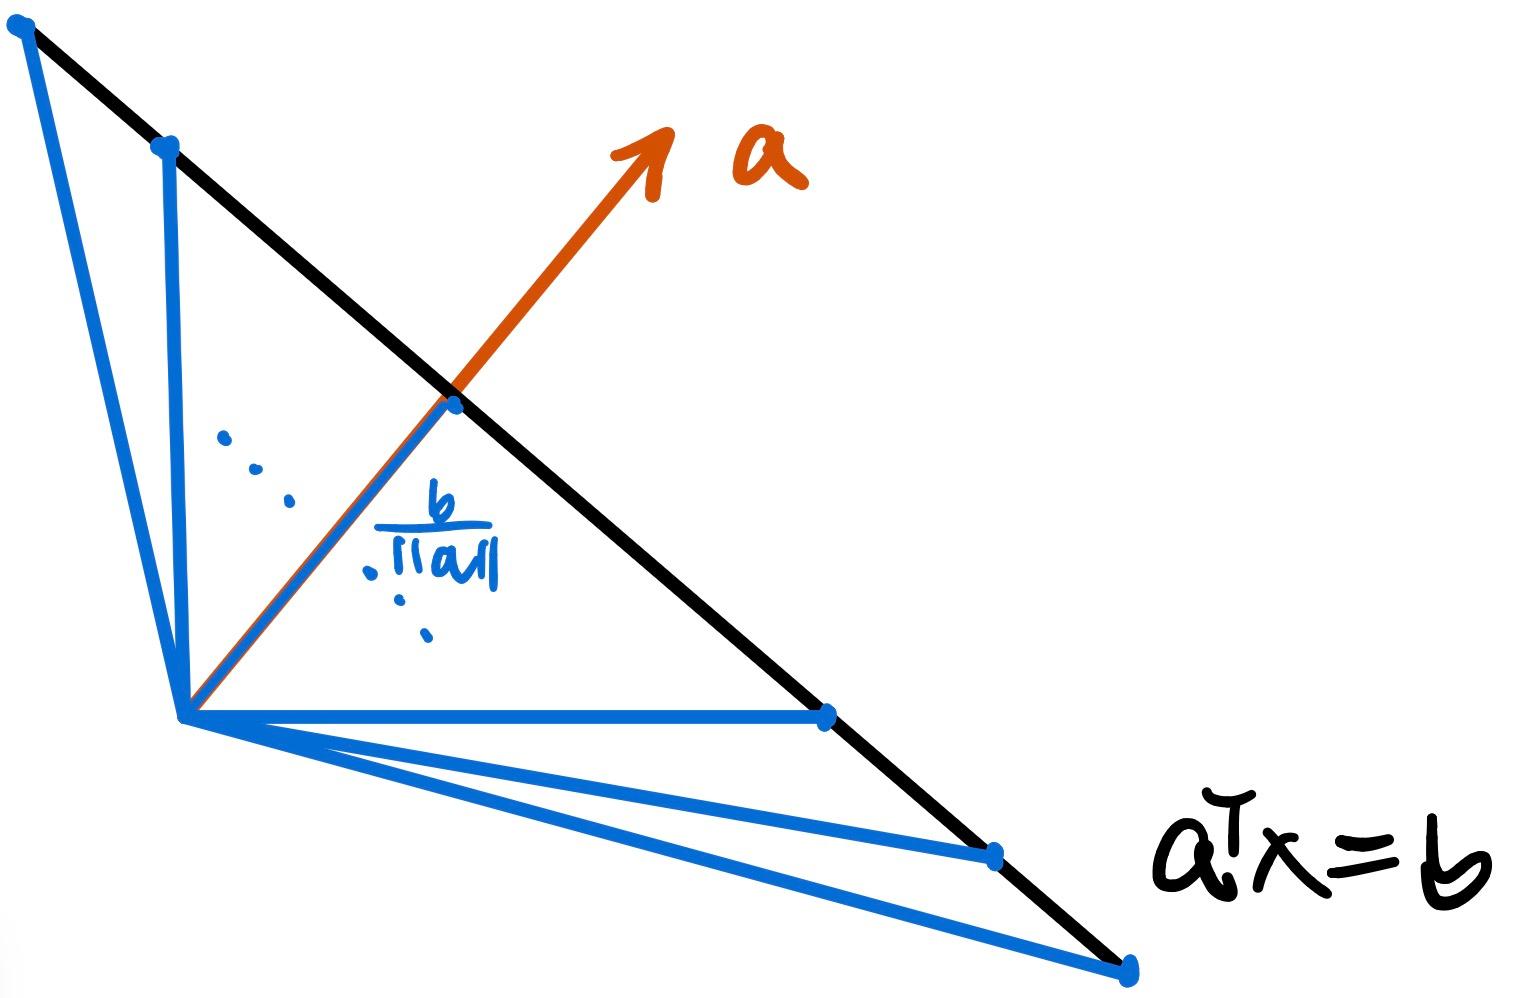
\includegraphics[width=0.3\linewidth]{figures/20260922111438897.png}
\end{center}


\end{itemize}

Closed halfspace:

\[
\mathcal{H}_- := \{\bm{x} \in \mathbb{R}^n: \bm{a}^\top \bm{x} \leq b\},\qquad \mathcal{H}_+ := \{\bm{x} \in \mathbb{R}^n: \bm{a}^\top \bm{x} \geq b\}.
\]

\begin{itemize}
\item {}Closed halfspace 是一个凸集.


\end{itemize}

\end{defblock}


% Source Markdown lines 106–118
\begin{defblock}[{Norm ball, ellipsoid}]
任意范数 $\|\cdot\|$ 定义的以 $\bm{c} \in \mathbb{R}^n$ 为中心、$r > 0$ 为半径的 norm ball 是 convex set:

\[
\mathcal{B}(\bm{c}, r) := \{\bm{x} \in \mathbb{R}^n: \|\bm{x}-\bm{c}\| \leq r\}.
\]

\begin{itemize}
\item {}注意: $0<p<1$ 时 对应的 $\ell_p$-norm 是 quasi-norm, 其不满足严格 norm 要求的三角不等式. 此时对应的 $\ell_p$-ball 一般不是凸集.


\end{itemize}

Ellipsoid 是一个凸集, 给定 $\bm{P} \in \mathbb{S}_{++}^n$ 和 $\bm{c} \in \mathbb{R}^n$，定义椭球的标准形式:

\[
\mathcal{E}(\bm{c}, \bm{P}) := \{\bm{x} \in \mathbb{R}^n: (\bm{x}-\bm{c})^\top \bm{P}^{-1} (\bm{x}-\bm{c}) \leq 1\} = \{\bm{x} \in \mathbb{R}^n: \|\bm{P}^{-1/2}(\bm{x}-\bm{c})\|_2 \leq 1\}.
\]

\begin{itemize}
\item {}或等价地, 以 affine 形式定义为 $\mathcal{E} = \{\bm{c} + \bm{A}\bm{u}: \|\bm{u}\|_2 \leq 1\}$, 其中 $\bm{A} \in \mathbb{R}^{n \times n}$ 非奇异.


\end{itemize}

\end{defblock}


% Source Markdown lines 120–128
\begin{defblock}[{Polyhedron, polytope}]
有限个 closed halfspace 和 hyperplane 的交集是一个 polyhedron:

\[
\mathcal{P} := \{\bm{x} \in \mathbb{R}^n: \bm{A}\bm{x} \leq \bm{b}, \bm{C}\bm{x} = \bm{d}\},
\]

\begin{itemize}
\item {}Polyhedron 和 polytope 都是凸集.


\item {}二者的说法有时会混用, 但严格说: polyhedron 可以是无界的, 而 polytope 是有界的.


\end{itemize}

\end{defblock}


% Source Markdown lines 130–147
\begin{defblock}[{Simplex}]
若 $\bm{v}_0, \ldots, \bm{v}_k \in \mathbb{R}^n$ 是 affinely independent 的点 (即 $\bm{v}_1-\bm{v}_0, \ldots, \bm{v}_k-\bm{v}_0$ 线性无关), 则称

\[
\mathcal{S} := \text{conv}\{\bm{v}_0, \ldots, \bm{v}_k\} 
\]

是一个 $k$-simplex.

\begin{itemize}
\item {}Affine independent 可以理解为, 给定一个参考点 $\bm{v}_0$，与其余点构成的向量是线性无关的. 因此这与其所处的空间维度是有密切联系的. 例如在二维平面中, 3 个点不共线, 给定一个参考点, 其余两个点可以 span 整个平面; 然而如果有四个点, 则必定会有一个点是冗余的. \textbf{在 $n$ 维空间中, 最多只能有 $n+1$ 个 affinely independent 的点.} (这些点 span 出了一个 $n$-dimensional affine space)


\item {}Simplex 是一种特殊的 polytope. 其相当于在对应 affine space 中最小 polytope. 其具有\textbf{唯一表出}的性质:

\[
\bm{x} \in \mathcal{S} \implies \bm{x} = \sum_{i=0}^k \theta_i \bm{v}_i,~ \text{ exists unique } \theta_i \geq 0, \sum_{i=0}^k \theta_i = 1.
\]

也鉴于这种性质, 可以考虑如下 $d$ 维 simplex 的标准形式:

\[
\Delta_d := \left\{\bm{\lambda} \in \mathbb{R}^{d+1}: \sum_{i=0}^d \lambda_i = 1,~ \lambda_i \geq 0,~ i=0,\ldots,d\right\}.
\]

其对应的 vertices 为 $\bm{e}_0, \ldots, \bm{e}_d$，其中 $\bm{e}_i$ 是 $(d+1)$ 维单位向量. 因此任意 $d$-dimensional simplex $\mathcal{S}$ 都存在一个 affine map $\Delta_d \to \mathcal{S}$，因此所有 $d$-dimensional simplex 都是 affine equivalent 的. 后面可以看到, 这种唯一表出的性质就可以让我们用来定义坐标系 (barycentric coordinates).


\end{itemize}

\end{defblock}


% Source Markdown lines 150–155
\begin{defblock}[{Convex cone}]
一个集合 $\mathcal{K}$ 若满足: $\bm{x} \in \mathcal{K}, \theta \geq 0 \implies \theta \bm{x} \in \mathcal{K}$, 则称 $\mathcal{K}$ 是一个 cone. 若 $\mathcal{K}$ 还是一个 convex set, 则称 $\mathcal{K}$ 是一个 convex cone. Convex cone 满足:

\[
\bm{x}_1, \bm{x}_2 \in \mathcal{K},~ \theta_1, \theta_2 \geq 0 \implies \theta_1 \bm{x}_1 + \theta_2 \bm{x}_2 \in \mathcal{K}.
\]

\end{defblock}

\begin{itemize}
\item {}考虑平面直角坐标系中的 $x$,$y$ 两个正半轴 $\{(t,0), t \geq 0\} \cup \{(0,t), t \geq 0\}$，则其是一个 cone, 但不是 convex cone. 若考虑整个象限 $\mathbb{R}_+^n := \{\bm{x} \in \mathbb{R}^n: x_i \geq 0, i=1,\ldots,n\}$，则其是一个 convex cone.


\end{itemize}


% Source Markdown lines 159–168
\begin{defblock}[{Second-order cone}]
\begin{itemize}
\item {}Second-order cone (SOC) 是一个 convex cone, 定义为:

\[
\mathcal{Q}^{n+1} := \{(t, \bm{x}) \in \mathbb{R}^{n+1}: t \geq \|\bm{x}\|_2\}.
\]

\begin{itemize}
\item {}SOC 是一个重要的 convex cone，它在优化问题中经常出现. 考虑 nonlinear 约束:

\[
\|\bm{A}\bm{x} + \bm{b}\|_2 \leq \bm{c}^\top \bm{x} + d,
\]

其中 $\bm{A} \in \mathbb{R}^{m \times n}$, $\bm{b} \in \mathbb{R}^m$, $\bm{c} \in \mathbb{R}^n$, $d \in \mathbb{R}$. 这就是一个 SOC 约束.


\end{itemize}


\end{itemize}

\end{defblock}


% Source Markdown lines 169–177
\begin{defblock}[{Positive semidefinite cone}]
\begin{itemize}
\item {}Positive semidefinite cone (PSD cone) 是一个 convex cone, 定义为:

\[
\mathbb{S}_+^n := \{\bm{X} \in \mathbb{S}^n: \bm{X} \succeq 0\},
\]

即对称半正定矩阵本身就是一个 convex cone. 一个典型的 SDP 问题即为:

\[
\min_{\bm{X}} \langle \bm{C}, \bm{X} \rangle \quad \text{s.t.} \quad \langle \bm{A}_i, \bm{X} \rangle = b_i,~ i=1,\ldots,m,~ \bm{X} \succeq 0.
\]

其中 $\bm{C}, \bm{A}_i \in \mathbb{S}^n$, $i=1,\ldots,m$, $\bm{X} \in \mathbb{S}^n$.


\end{itemize}

\end{defblock}


% Source Markdown lines 179–183
\begin{defblock}[{Conic optimization}]
总的而言, conic optimization 是一个重要的优化问题类别, 其形式为:

\[
\min_{\bm{x}} \langle \bm{c}, \bm{x} \rangle \quad \text{s.t.} \quad \bm{A}\bm{x} = \bm{b},~ \bm{x} \in \mathcal{K},
\]

其中 $\mathcal{K}$ 是一个 convex cone. 其包含了 LP, SOCP, SDP 等优化问题.

\end{defblock}

\textbf{Cone 是一种广义的非负.} simplex 主要讨论的是一种位置关系, 而 cone 主要讨论的是一种方向关系. 对应的, simplex 会关心 extreme points, 而 cone 会关心 extreme rays.

\subsubsection{保凸运算}


% Source Markdown lines 190–196
\begin{propositionblock}[{保凸运算}]
实践中往往不会通过定义来验证给定复杂集合的凸性, 而是通过一些基本凸集出发, 通过一些保凸运算来构造新的凸集. 给定指标集合 $\mathcal{I}$，任意 $\mathcal{C}, \mathcal{C}_i \subseteq \mathbb{R}^n$，$i \in \mathcal{I}$ 是凸集, 则有以下保凸运算:

\begin{itemize}
\item {}任意交集: $\bigcap_{i \in \mathcal{I}} \mathcal{C}_i$ 是凸集.


\item {}仿射映射: 若 $\bm{A} \in \mathbb{R}^{m \times n}$ 且 $\bm{b} \in \mathbb{R}^m$，则 $\bm{A}\mathcal{C} + \bm{b} := \{\bm{A}\bm{x} + \bm{b}: \bm{x} \in \mathcal{C}\}$ 是凸集.


\item {}仿射的 preimage: 若 $\bm{A} \in \mathbb{R}^{m \times n}$ 且 $\bm{b} \in \mathbb{R}^m$，且这里 $\mathcal{C} \subseteq \mathbb{R}^m$, 则 $\{\bm{x} \in \mathbb{R}^n: \bm{A}\bm{x} + \bm{b} \in \mathcal{C}\}$ 是凸集.


\item {}Minkowski sum: $\mathcal{C}_1 + \mathcal{C}_2 := \{\bm{x}_1 + \bm{x}_2: \bm{x}_1 \in \mathcal{C}_1, \bm{x}_2 \in \mathcal{C}_2\}$ 是凸集.


\item {}Cartesian product: $\mathcal{C}_1 \times \mathcal{C}_2 := \{(\bm{x}_1, \bm{x}_2): \bm{x}_1 \in \mathcal{C}_1, \bm{x}_2 \in \mathcal{C}_2\}$ 是凸集.


\item {}Projection: 若 $\mathcal{C} \subseteq \mathbb{R}^{n+m}$ 是凸集, 则将 $\mathcal{C}$ 投影到 $\bm{x}$ 上得到 $\Pi_x \mathcal{C} := \{\bm{x} \in \mathbb{R}^n:  \exists \bm{y} \in \mathbb{R}^m, \text{s.t. } (\bm{x}, \bm{y}) \in \mathcal{C}\}$ 是凸集.


\end{itemize}

\end{propositionblock}

\subsection{Carathéodory's theorem}

在正式给出 Carathéodory 定理之前, 先明确 \textbf{affine space} 的概念.


% Source Markdown lines 202–206
\begin{defblock}[{Affine space}]
\begin{itemize}
\item {}Affine space 可以理解为一个平移后的线性子空间, 或一个不经过(也不关心)原点的线性子空间, 即 $\mathcal{A} = \bm{x}_0 + \mathcal{V}$, 其中 $\mathcal{V}$ 是一个线性子空间, $\bm{x}_0$ 是一个固定点.


\item {}或者这么说, 本身 affine-linear 就是一组类似相对应的词汇. affine 是有截距的 linear.


\item {}所以比如前文在讨论 simplex 时, 说 $\bm{v}_0, \ldots, \bm{v}_k$ 是 affinely independent 的点, 也就是说 $\text{aff}(\{\bm{v}_0, \ldots, \bm{v}_k\})$ 是一个 $k$-dimensional affine space.


\item {}在后面的认知当中, 也可以区分 affine dimension 和 ambient dimension. Ambient dimension 可以粗略的理解为就是所在客观世界的维度, 其可能是很大的. 而 affine dimension 是指真正我们关注的比如 feasible region $\mathcal{S}$ 所在的 affine space 的维度. 若 $\mathcal{S}$ 位于一个 $m$-dimensional affine space 中, 则即使整个空间是很高维的, 我们也只需要 $m+1$ 个点就可以表示出任意一个凸组合.


\end{itemize}

\end{defblock}


% Source Markdown lines 208–208
\begin{thmblock}[{Carathéodory}]
设 $\mathcal{S} \subseteq \mathbb{R}^n$. 若 $\bm{x} \in \text{conv}(\mathcal{S})$，则 $\bm{x}$ 可以表示为 $\mathcal{S}$ 中至多 $n+1$ 个点的凸组合. $^\dagger$ 也即, 若 $\mathcal{S} \subseteq \mathbb{R}^n$，$\text{dim}~\text{aff}(\text{conv}(\mathcal{S})) = m$，那么对任意 $\bm{x} \in \text{conv}(\mathcal{S})$，存在至多 $m+1$ 个点 $\bm{x}_1, \ldots, \bm{x}_{k} \in \mathcal{S}$ ($k \leq m+1$) 和系数 $\theta_1, \ldots, \theta_k \geq 0$，使得 $\sum_{i=1}^k \theta_i = 1$ 且 $\bm{x} = \sum_{i=1}^k \theta_i \bm{x}_i$.

\end{thmblock}

\begin{itemize}
\item {}直观理解, 在 $n$ 维空间中, 最多只需要 $n+1$ 个点就可以表示出任意一个凸组合. 其实这个 theorem 有点类似 simplex 的反向理解.


\end{itemize}


% Source Markdown lines 213–220
\begin{proof}{}
$~^\dagger$ \emph{[Nemirovski, Appendix. B §B.2.1]} :

\begin{itemize}
\item {}由于 $\bm{x} \in \text{conv}(\mathcal{S})$，一定存在有限 $N$, 使得 $\bm{x} = \sum_{i=1}^N \theta_i \bm{x}_i$，其中 $\bm{x}_i \in \mathcal{S}$, $\theta_i \geq 0$, $\sum_{i=1}^N \theta_i = 1$. 并且选取所有可能构造中目前最小的 $N$ (例如去掉一些 $\theta_i = 0$ 的点).


\item {}下证明, 定有 $N \leq m+1$. 用反证法, 假设 $N > m+1$. 此时由于 $\bm{x}_1, \ldots, \bm{x}_N$ 在 $m$-dimensional affine space 中, 定是 affine dependent 的, 即存在 $\alpha_1, \ldots, \alpha_N$ 不全为零, 且 $\sum_{i=1}^N \alpha_i = 0$, 使得 $\sum_{i=1}^N \alpha_i \bm{x}_i = 0$.


\item {}故根据 $\sum_{i=1}^N \theta_i = 1$ 和 $\sum_{i=1}^N \alpha_i = 0$，有 $\sum_{i=1}^N (\theta_i + t\alpha_i) = 1$ 对任意 $t \in \mathbb{R}$ 成立. 同时, $\sum_{i=1}^N (\theta_i + t\alpha_i) \bm{x}_i = \sum_{i=1}^N \theta_i \bm{x}_i + t\sum_{i=1}^N \alpha_i \bm{x}_i = \bm{x}$ 对任意 $t \in \mathbb{R}$ 成立.


\item {}因此我们总可以通过调整 $t$ 来得到一个新的凸组合, 使得至少有一个新的系数为零, 也即我们可以去掉一个点, 这与我们选取的最小 $N$ 矛盾. 因此定有 $N \leq m+1$.


\end{itemize}

\end{proof}

\subsection{Basic Topologies}

在优化过程中, 算法总是会产生一系列的迭代点 $\bm{x}_1, \bm{x}_2, \ldots$，我们希望 $\bm{x}_k \to \bm{x}^\star$ 收敛到一个最优解 $\bm{x}^\star$. 因此会有一系列问题: 如果 $\bm{x}_k \in \mathcal{S}$ 且 $\bm{x}_k \to \bm{x}^\star$，是否有 $\bm{x}^\star \in \mathcal{S}$? 如果 $f(\bm{x}_k) \to \inf f$, 是否有 $\bm{x}^\star \in \mathcal{S}$ 且 $f(\bm{x}^\star) = \inf f$? 这些问题都与集合的拓扑性质有关.

给定 norm ball $\mathcal{B}(\bm{x}, \varepsilon) := \{\bm{y} \in \mathbb{R}^n: \|\bm{y}-\bm{x}\| \leq \varepsilon\}$.在欧式空间中, 任意 norm 都是等价的.

首先考虑如下几个基本的集合拓扑概念. 给定 $S \subseteq \mathbb{R}^n$:


% Source Markdown lines 230–246
\begin{defblock}[{Basic topologies}]
\begin{itemize}
\item {}$\text{int}(\mathcal{S}) := \{\bm{x} \in \mathcal{S}: \exists \varepsilon > 0, \mathcal{B}(\bm{x}, \varepsilon) \subseteq \mathcal{S}\}$.

\begin{itemize}
\item {}$\bm{x}$ 是集合的内点, 说明存在一个小邻域完全包含在集合中.


\item {}集合 $\mathcal{S}$ 是 open set 当且仅当 $\mathcal{S} = \text{int}(\mathcal{S})$, 即集合的任意点都是内点.


\end{itemize}


\item {}$\text{cl}(\mathcal{S}) := \{\bm{x} \in \mathbb{R}^n: \forall \varepsilon > 0, \mathcal{B}(\bm{x}, \varepsilon) \cap \mathcal{S} \neq \emptyset\}$.

\begin{itemize}
\item {}集合的闭包可以认为是集合+集合的极限点.


\item {}$\bm{x} \in \text{cl}(\mathcal{S})$ 当且仅当存在一个序列 $\{\bm{x}_k\} \subseteq \mathcal{S}$ 使得 $\bm{x}_k \to \bm{x}$. 所有从 $\mathcal{S}$ 中的点构成的极限点都包含在 $\text{cl}(\mathcal{S})$ 中.


\item {}集合 $\mathcal{S}$ 是 closed set 当且仅当 $\mathcal{S} = \text{cl}(\mathcal{S})$, 即集合包含其所有极限点.


\end{itemize}


\item {}$\partial \mathcal{S} := \text{cl}(\mathcal{S}) \setminus \text{int}(\mathcal{S})$.

\begin{itemize}
\item {}集合的边界是集合的闭包减去集合的内点.


\item {}$\mathcal{B}(\bm{x}, \varepsilon) \cap \mathcal{S} \neq \emptyset$ 且 $\mathcal{B}(\bm{x}, \varepsilon) \cap (\mathbb{R}^n \setminus \mathcal{S}) \neq \emptyset$ 对任意 $\varepsilon > 0$ 成立, 则 $\bm{x}$ 是集合的边界点.


\end{itemize}


\item {}$\mathcal{S}$ 是 bounded set 当且仅当存在 $M > 0$ 使得 $\|\bm{x}\| \leq M$ 对所有 $\bm{x} \in \mathcal{S}$ 成立.


\item {}有限维欧式空间中, $\mathcal{S}$ 是 compact set 当且仅当 $\mathcal{S}$ 是 closed 且 bounded (Heine-Borel theorem).

\begin{itemize}
\item {}在优化视角, \textbf{$\mathcal{S}$ 是 compact set 当且仅当 $\mathcal{S}$ 中任何一个序列都存在一个收敛的子序列, 且其极限点仍然在 $\mathcal{S}$ 中.} 这保证了集合内迭代点列存在收敛子列.

\begin{itemize}
\item {}(Bolzano-Weierstrass theorem 保证任何有界序列都存在收敛子序列. 而 compactness 保证了收敛子序列的极限点仍然在集合中.)


\end{itemize}


\item {}Compactness 在优化中避免了如下两种最优解求解失败之场景:

\begin{itemize}
\item {}集合不闭: 例如 $\min_{x \in (0,1)} x$，其 infimum 为 $0$，但 $0 \notin (0,1)$.


\item {}集合不有界: 例如 $\min_{x \geq 0} \exp(-x)$，其 infimum 为 $0$，但取在 $x \to \infty$.


\end{itemize}


\end{itemize}


\end{itemize}

\end{defblock}

接着引入 \textbf{relative interior} 的概念.


% Source Markdown lines 249–260
\begin{defblock}[{Relative interior}]
\begin{itemize}
\item {}给定集合 $\mathcal{S} \subseteq \mathbb{R}^n$，其 affine hull 为 $\text{aff}(\mathcal{S})$. 定义 $\mathcal{S}$ 的相对内点为:

\[
\text{ri}(\mathcal{S}) := \{\bm{x} \in \mathcal{S}: \exists \varepsilon > 0, \mathcal{B}(\bm{x}, \varepsilon) \cap \text{aff}(\mathcal{S}) \subseteq \mathcal{S}\}.
\]


\item {}Intuition: 考虑一个 $\mathbb{R}^3$ 中的二维 simplex $\Delta_2$. 显然, $\text{int}(\Delta_2) = \emptyset$, 因为三维空间内的任意球体都无法完全包含在一个二维的平面中. 但是这显然并不是我们关心的. 我们只需要考虑这个我们关注集合 $\mathcal{S}$ 所在的 affine space, 然后考虑 ambient space 中的球体与 affine space 的公共部分, 讨论这个公共部分的内点情况即可.


\item {}Relative interior 帮助我们能够良好的处理在高维空间内的低维集合之间的关系.


\item {}反过来也可以定义 relative boundary, 即 $\partial_{\text{rel}}(\mathcal{S}) := \text{cl}(\mathcal{S}) \setminus \text{ri}(\mathcal{S})$.


\end{itemize}

故有关系:

\[
\text{ri}(\mathcal{S}) \subseteq \mathcal{S} \subseteq \text{cl}(\mathcal{S}) \subseteq \text{aff}(\mathcal{S}),
\]

\end{defblock}


% Source Markdown lines 262–268
\begin{propositionblock}[{Relative interior of a convex set}]
\begin{itemize}
\item {}对于非空 convex set $\mathcal{C} \subseteq \mathbb{R}^n$，有 $\text{ri}(\mathcal{C}) \neq \emptyset$, $\text{ri}(\text{cl}(\mathcal{C})) = \text{ri}(\mathcal{C})$, $\text{cl}(\text{ri}(\mathcal{C})) = \text{cl}(\mathcal{C})$.


\item {}此外, 若 $\bm{x} \in \text{ri}(\mathcal{C})$ 且 $\bm{y} \in \text{cl}(\mathcal{C})$，则

\[
(1-t) \bm{x} + t \bm{y} \in \text{ri}(\mathcal{C}),~ \forall t \in [0,1).
\]

即从相对内点出发, 向任意闭包点连线, 只要没有到达闭包点, 都会落在相对内点中.


\end{itemize}

\end{propositionblock}

\subsection{Weierstrass theorem, existence of optimal solution}

\subsubsection{Weierstrass theorem}


% Source Markdown lines 274–278
\begin{thmblock}[{Weierstrass}]
若 $\mathcal{S} \subseteq \mathbb{R}^n$ 是非空的 \textbf{compact} set, 且 $f: \mathcal{S} \to \mathbb{R}$ 是\textbf{连续}函数, 则 $f$ 在 $\mathcal{S}$ 上有最小和最大值. 特别地, 存在 $\bm{x}^\star \in \mathcal{S}$ 使得

\[
f(\bm{x}^\star) = \min_{\bm{x} \in \mathcal{S}} f(\bm{x}).
\]

\end{thmblock}

\begin{itemize}
\item {}Tl;dr: 可行域紧 + 目标函数连续 $\implies$ 存在最优解.


\item {}优化中, 证明最优解存在的通常思路:

\begin{itemize}
\item {}证明 feasible set 是紧的


\item {}即使 feasible set 是 unbounded, 但存在某个非空 sublevel set $\{\bm{x} \in \mathcal{S}: f(\bm{x}) \leq \alpha\}$ 是紧的, 则可以将问题限制在这个 sublevel set 上


\end{itemize}


\end{itemize}


% Source Markdown lines 284–284
\begin{proof*}[{Proof Sketch}]
令 $\alpha := \inf_{\bm{x} \in \mathcal{S}} f(\bm{x})$. 选择一个序列 $\{\bm{x}_k\} \subseteq \mathcal{S}$ 使得 $f(\bm{x}_k) \downarrow \alpha$. 因为 $\mathcal{S}$ 是 compact set, $\{\bm{x}_k\}$ 有一个收敛的子序列 $\{\bm{x}_{k_j}\} \to \bm{x}^\star \in \mathcal{S}$. 由于 $f$ 是连续函数, 则 $f(\bm{x}_{k_j}) \to f(\bm{x}^\star)$. 因此 $f(\bm{x}^\star) = \alpha$, 即 $\bm{x}^\star$ 是最优解.

\end{proof*}


% Source Markdown lines 286–295
\begin{proof}{}
\emph{[Beck, Ch. 2]}:

\begin{quote}
\emph{在 Beck 的论述中, 其将 Weierstrass theorem 的条件, 从 $f: S \to \mathbb{R}$ 是连续函数, 放宽为 $f$ 是 proper 且 closed 函数. 这是一个更弱的条件, 但其证明思路是类似的.}

\end{quote}

\begin{itemize}
\item {}\textbf{先证 $f$ bounded below}. \emph{在 sketch 中我们直接定义 $\alpha := \inf_{\bm{x} \in \mathcal{S}} f(\bm{x})$. 然而这个 inf 是有限实数本身也是需要严格证明的.} 即, 要证: 存在 $L \in \mathbb{R}$ 使得 $f(\bm{x}) \geq L$ 对所有 $\bm{x} \in \mathcal{S}$ 成立.

\begin{itemize}
\item {}反证法, 假设 $f$ 不存在下界, 则对于每一个正整数 $k$, 都可以找到 $\bm{x}_k \in \mathcal{S}$ 使得 $f(\bm{x}_k) \leq -k$. 于是我们可以构造一个序列 $\{\bm{x}_k\} \subseteq \mathcal{S}$ 使得 $f(\bm{x}_k) \to -\infty$. 由于 $\mathcal{S}$ 是 compact set, $\{\bm{x}_k\}$ 有一个收敛的子序列 $\{\bm{x}_{k_j}\} \to \bar{\bm{x}} \in \mathcal{S}$. 由于 $f$ 是连续函数且 $\bm{x}_{k_j} \to \bar{\bm{x}}$，则 $f(\bm{x}_{k_j}) \to f(\bar{\bm{x}})$ 是一个有限值. 然而 $f(\bm{x}_{k_j}) \to -\infty$, 这与 $f(\bar{\bm{x}})$ 是有限值矛盾.


\end{itemize}


\item {}\textbf{再证 $f$ 在 $\mathcal{S}$ 上有最小值}. 由实数完备性, $f$ 有下界故有下确界, 记 $\alpha := \inf_{\bm{x} \in \mathcal{S}} f(\bm{x})$. 下证 $\exists \bm{x}^\star \in \mathcal{S}$ 使得 $f(\bm{x}^\star) = \alpha$. 由 inf 的定义, 对于每个 $k \geq 1$, 都存在 $\bm{x}_k \in \mathcal{S}$ 使得 $\alpha \leq f(\bm{x}_k) < \alpha + 1/k$. 由 squeeze theorem 可以给出 $f(\bm{x}_k) \to \alpha$. 再次由于 $\mathcal{S}$ 是 compact set, $\{\bm{x}_k\}$ 有一个收敛的子序列 $\{\bm{x}_{k_j}\} \to \bm{x}^\star \in \mathcal{S}$. 由于 $f$ 是连续函数, 则 $f(\bm{x}_{k_j}) \to f(\bm{x}^\star)$. 因此 $f(\bm{x}^\star) = \alpha$, 即 $\bm{x}^\star$ 是最优解.


\end{itemize}

\end{proof}


% Source Markdown lines 297–297
\begin{colblock}[{强凸函数在闭凸集上的最优解存在且唯一}]
[Yurii, $\S$ 2.2.3, Thm. 2.2.10] \emph{(强凸函数在闭凸集上的最优解存在且唯一)}: 若 $\mathcal{Q} \subseteq \mathbb{R}^n$ 是非空的 closed convex set, 且 $f: \mathcal{Q} \to \mathbb{R}$ 是 $\mu$-strongly convex 函数 (即 $\exists \mu > 0$ 使得 $f(\bm{y}) \geq f(\bm{x}) + \nabla f(\bm{x})^\top (\bm{y}-\bm{x}) + \frac{\mu}{2}\|\bm{y}-\bm{x}\|_2^2,~ \forall \bm{x}, \bm{y} \in \mathcal{Q}$), 且 $f$ 是连续的, 则 $\min_{\bm{x} \in \mathcal{Q}} f(\bm{x})$ 存在唯一最优解.

\end{colblock}

\section{Projections}

\subsection{Euclidean projection}


% Source Markdown lines 305–312
\begin{defblock}[{Euclidean distance and projection}]
给定非空闭集 $\mathcal{C} \subseteq \mathbb{R}^n$，定义点 $\bm{x} \in \mathbb{R}^n$ 到集合 $\mathcal{C}$ 的 Euclidean distance 为:

\[
d(\bm{x}, \mathcal{C}) := \inf_{\bm{y} \in \mathcal{C}} \|\bm{x}-\bm{y}\|_2.
\]

若存在 $\bm{y}^\star \in \mathcal{C}$ 使得 $d(\bm{x}, \mathcal{C}) = \|\bm{x}-\bm{y}^\star\|_2$，则称 $\bm{y}^\star$ 是 $\bm{x}$ 在 $\mathcal{C}$ 上的 Euclidean projection, 记为:

\[
\Pi_{\mathcal{C}}(\bm{x}) := \arg\min_{\bm{y} \in \mathcal{C}} \|\bm{x}-\bm{y}\|_2.
\]

\end{defblock}


% Source Markdown lines 314–314
\begin{thmblock}[{凸闭集上的投影存在唯一}]
若 $\mathcal{C} \subseteq \mathbb{R}^n$ 是非空, 闭, 凸的, 则对每个 $\bm{y} \in \mathbb{R}^n$，存在唯一的 $\bm{x}^\star \in \mathcal{C}$ 使得 $\bm{x}^\star = \Pi_{\mathcal{C}}(\bm{y})$.

\end{thmblock}


% Source Markdown lines 316–352
\begin{proof}{}
证明等价于证明 $\min_{\bm{x} \in \mathcal{C}} \|\bm{x}-\bm{y}\|_2^2$ 存在唯一最优解.

存在性.

\begin{center}
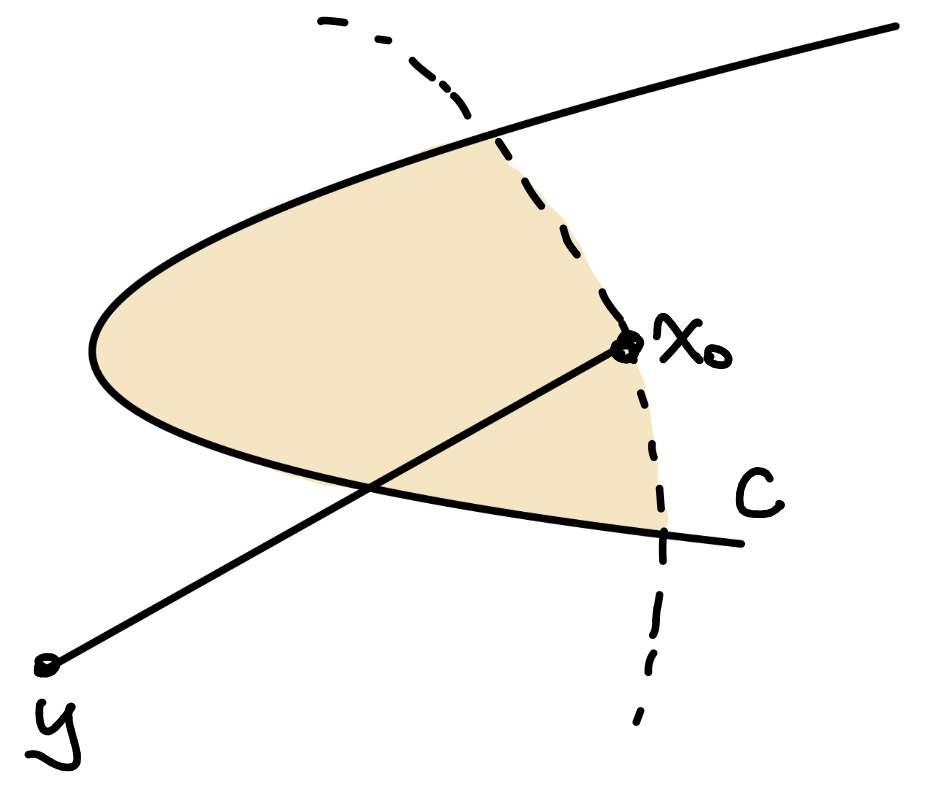
\includegraphics[width=0.3\linewidth]{figures/20260929111038580.png}
\end{center}

\begin{itemize}
\item {}根据 Weierstrass theorem, 由于目标函数是连续的, 故只需给出一个紧的可行域即可. Compact = closed + bounded, 而 closed 已经给出, 故只需找到一个 bounded 的可行域即可.


\item {}由于 $\mathcal{C}$ 是非空闭集, 故任取 $\bm{x}_0 \in \mathcal{C}$, 记 $R:= \|\bm{x}_0 - \bm{y}\|_2$. 则任意 $d(\bm{x}, \bm{y}) > R$ 的点 $\bm{x} \in \mathcal{C}$ 都不可能是最优解. 故可行域为 $\mathcal{C} \cap \mathcal{B}(\bm{y}, R)$，其是一个非空闭集, 且 bounded, 故是 compact set. 因此最优解存在.


\end{itemize}

唯一性. 事实上唯一性在证明, 对于凸可行域+强凸目标函数, 其最优解若存在必然唯一.

\begin{itemize}
\item {}反证法, 若存在两个不同的最优解 $\bm{x}_1^\star, \bm{x}_2^\star \in \mathcal{C}$，一方面

\[
\begin{aligned}
  \|\bm{y} - \bm{x}_1^\star + (\bm{y} - \bm{x}_2^\star)\|_2^2 &= \|\bm{y} - \bm{x}_1^\star\|_2^2 + \|\bm{y} - \bm{x}_2^\star\|_2^2 + 2\left\langle \bm{y} - \bm{x}_1^\star, \bm{y} - \bm{x}_2^\star \right\rangle\\
\end{aligned}
\]

另一方面

\[
\begin{aligned}
  \|\bm{y} - \bm{x}_1^\star - (\bm{y} - \bm{x}_2^\star)\|_2^2 &= \|\bm{x}_1^\star - \bm{x}_2^\star\|_2^2 = \|\bm{x}_1^\star - \bm{y}\|_2^2 + \|\bm{x}_2^\star - \bm{y}\|_2^2 - 2\left\langle \bm{y} - \bm{x}_1^\star , \bm{y} - \bm{x}_2^\star \right\rangle\\
\end{aligned}
\]

因此由第二式整理得

\[
\left\langle \bm{y} - \bm{x}_1^\star, \bm{y} - \bm{x}_2^\star \right\rangle = d(\bm{y}, \mathcal{C})^2 -\frac{1}{2}\|\bm{x}_1^\star - \bm{x}_2^\star\|_2^2 < d(\bm{y}, \mathcal{C})^2.
\]


\item {}考虑 $\bm{y}$ 到 $\frac{1}{2}(\bm{x}_1^\star + \bm{x}_2^\star)$ 的距离, 由于 $\mathcal{C}$ 是凸的, 必有 $\frac{1}{2}(\bm{x}_1^\star + \bm{x}_2^\star) \in \mathcal{C}$. 于是

\[
\begin{aligned}
  \|\bm{y} - \frac{1}{2}(\bm{x}_1^\star + \bm{x}_2^\star)\|_2^2 &= \left\|\frac{1}{2}(\bm{y}-\bm{x}_1^\star) + \frac{1}{2}(\bm{y}-\bm{x}_2^\star)\right\|_2^2\\
  &= \frac{1}{4}\|\bm{y}-\bm{x}_1^\star\|_2^2 + \frac{1}{4}\|\bm{y}-\bm{x}_2^\star\|_2^2 + \frac{1}{2}\left\langle \bm{y}-\bm{x}_1^\star, \bm{y}-\bm{x}_2^\star \right\rangle\\
  &< \frac{1}{4}\|\bm{y}-\bm{x}_1^\star\|_2^2 + \frac{1}{4}\|\bm{y}-\bm{x}_2^\star\|_2^2 + \frac12 d(\bm{y}, \mathcal{C})^2 = d(\bm{y}, \mathcal{C})^2.
\end{aligned}
\]

这与 $\bm{x}_1^\star, \bm{x}_2^\star$ 是最优解矛盾. 因此最优解唯一.


\end{itemize}

\end{proof}

\subsection{Projection variational inequality}


% Source Markdown lines 357–361
\begin{thmblock}[{Projection variational inequality}]
对于非空闭凸集 $\mathcal{C} \subseteq \mathbb{R}^n$，$\bm{x}^\star \in \mathcal{C}$ 是 $\Pi_{\mathcal{C}}(\bm{y})$ 当且仅当

\[
\left\langle \bm{y} - \bm{x}^\star, \bm{x} - \bm{x}^\star \right\rangle \leq 0,~ \forall \bm{x} \in \mathcal{C}.
\]

\end{thmblock}

\begin{center}
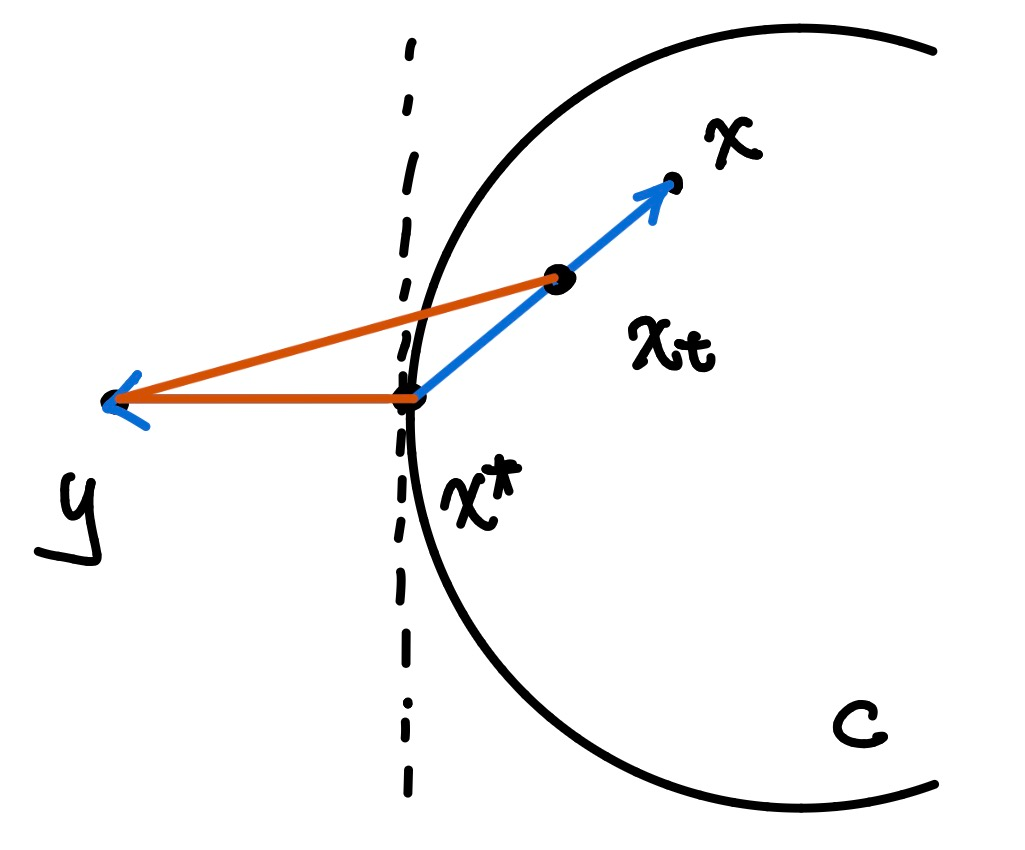
\includegraphics[width=0.3\linewidth]{figures/20260929215140832.png}
\end{center}

\begin{itemize}
\item {}从 $\bm{x}^\star$ 出发, 向投影起点的向量定与任意可行点的向量呈钝角或直角.


\end{itemize}


% Source Markdown lines 367–391
\begin{proof}{}
$(\Leftarrow)$ 对于任意 $\bm{x} \in \mathcal{C}$，有

\[
\begin{aligned}
\|\bm{y}-\bm{x}\|_2^2 &= \|\bm{y}-\bm{x}^\star + \bm{x}^\star - \bm{x}\|_2^2\\
&= \|\bm{y}-\bm{x}^\star\|_2^2 + \|\bm{x}^\star - \bm{x}\|_2^2 + 2\left\langle \bm{y}-\bm{x}^\star, \bm{x}^\star - \bm{x} \right\rangle\\
&\geq \|\bm{y}-\bm{x}^\star\|_2^2 + \|\bm{x}^\star - \bm{x}\|_2^2 \geq \|\bm{y}-\bm{x}^\star\|_2^2.
\end{aligned}
\]

故 $\bm{x}^\star = \arg\min_{\bm{x} \in \mathcal{C}} \|\bm{y}-\bm{x}\|_2 = \Pi_{\mathcal{C}}(\bm{y})$.

$(\Rightarrow)$ 定义 $\bm{x}_t := \bm{x}^\star + t(\bm{x}-\bm{x}^\star)$, $t \in(0,1]$. 由于 $\mathcal{C}$ 是凸的, 故 $\bm{x}_t \in \mathcal{C}$. 由 $\bm{x}^\star = \Pi_{\mathcal{C}}(\bm{y})$，有

\[
\begin{aligned}
\|\bm{y}-\bm{x}^\star\|_2^2 & \leq \|\bm{y}-\bm{x}_t\|_2^2 = \|\bm{y}-\bm{x}^\star + t(\bm{x}^\star - \bm{x})\|_2^2\\
& = \|\bm{y}-\bm{x}^\star\|_2^2 + t^2\|\bm{x}^\star - \bm{x}\|_2^2 + 2t\left\langle \bm{y}-\bm{x}^\star, \bm{x}^\star - \bm{x} \right\rangle.
\end{aligned}
\]

消去两边共同的平方距离项后, 左右两边同时除以 $t > 0$，并令 $t \downarrow 0$，则有

\[
\left\langle \bm{y}-\bm{x}^\star, \bm{x}^\star - \bm{x} \right\rangle \geq 0,~ \forall \bm{x} \in \mathcal{C}.
\]

\end{proof}

\subsection{Normal cone and optimality condition}

\subsubsection{Normal cone}

若进一步引入法锥 (normal cone) 的概念, 则可以将 projection variational inequality 进一步推广为更一般的 optimality condition.


% Source Markdown lines 399–402
\begin{defblock}[{Normal cone}]
定义闭凸集 $\mathcal{C} \subseteq \mathbb{R}^n$ 在 $\bm{x} \in \mathcal{C}$ 处的法锥为:

\[
\mathcal{N}_{\mathcal{C}}(\bm{x}) := \{\bm{v} \in \mathbb{R}^n: \left\langle \bm{v}, \bm{y}-\bm{x} \right\rangle \leq 0,~ \forall \bm{y} \in \mathcal{C}\}.
\]

\end{defblock}

\begin{itemize}
\item {}集合某点的法锥可以理解为从该点出发, 与任意可行位移都呈直角或钝角的向量的集合.


\item {}$\langle \bm{v}, \bm{y}-\bm{x} \rangle \leq 0$ 相当于是在寻找所有的直角或钝角向量. 因此每给定一个 $\bm{y} \in \mathcal{C}$，都会排除掉一半的空间. 最终被保留的部分的交集就是法锥.


\end{itemize}

如下是几种典型的法锥示意图:

\begin{center}
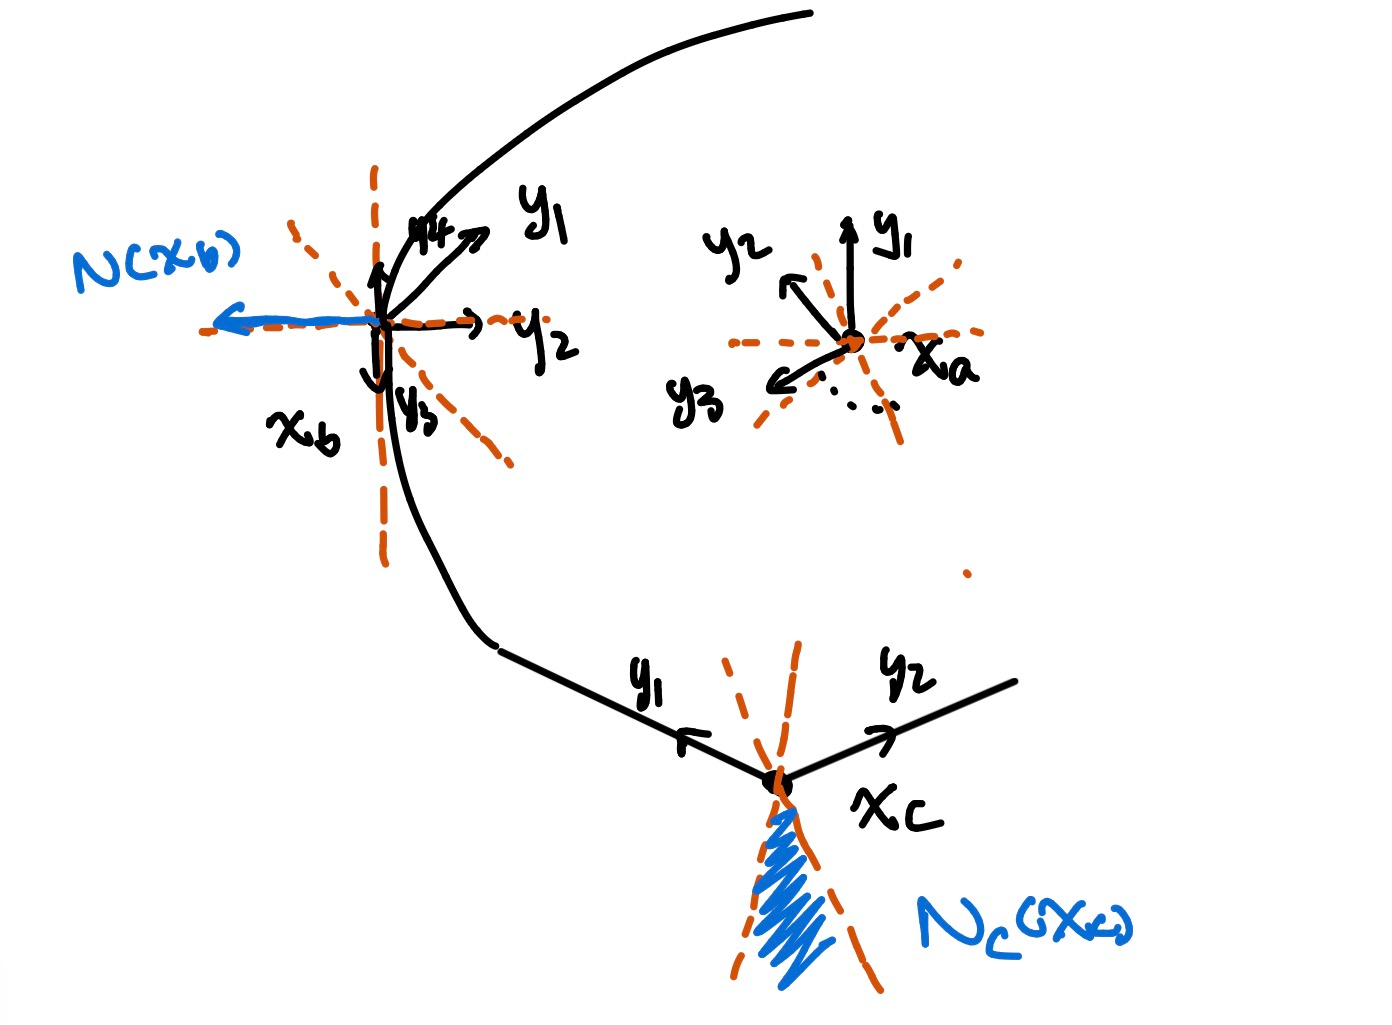
\includegraphics[width=0.5\linewidth]{figures/20260929221224372.png}
\end{center}

\begin{itemize}
\item {}$\bm{x}_a \in \text{int}(\mathcal{C})$ 是集合的内点. 则四周都是集合的点, 因此从 $\bm{x}_a$ 出发, 满足法向不等式的非零向量是不存在的. 因此 $\mathcal{N}_{\mathcal{C}}(\bm{x}_a) = \{\bm{0}\}$.


\item {}$\bm{x}_b \in \partial \mathcal{C}$ 是集合的边界点. 则从 $\bm{x}_b$ 出发, 指向集合外部的向量是存在的. 最极端考虑两个切线方向, 则从 $\bm{x}_b$ 出发, 指向集合外部的向量只能在这两个切线方向之间. 因此 $\mathcal{N}_{\mathcal{C}}(\bm{x}_b)$ 是一个射线, 其方向垂直于切线方向.


\item {}$\bm{x}_c \in \mathcal{C}$ 是集合的角点. 则法锥是构成角点的法向量的非负锥组合. 也即, 法锥是一个凸锥, 其包含了所有满足上述法向不等式的向量.


\end{itemize}

\emph{\textbf{法锥与投影}}


% Source Markdown lines 418–425
\begin{propositionblock}[{法锥与投影}]
Projection variational inequality 可以用法锥的概念来重新表述为:

\[
\bm{x}^\star = \Pi_{\mathcal{C}}(\bm{y}) \iff \bm{y}-\bm{x}^\star \in \mathcal{N}_{\mathcal{C}}(\bm{x}^\star).
\]

或

\[
\bm{y} - \Pi_{\mathcal{C}}(\bm{y}) \in \mathcal{N}_{\mathcal{C}}(\Pi_{\mathcal{C}}(\bm{y})).
\]

\end{propositionblock}

\emph{\textbf{法锥与超平面}}

此外, 回顾一个超平面的定义 $\{\bm{x} \in \mathbb{R}^n: \bm{a}^\top \bm{x} = b\}$, 其法向量就是 $\bm{a}$. 因此确定了一个法向量就确定了一个平面的方向, 再加上平面过的一个点, 就确定了一个超平面. 而对于法锥中的法向量, 这样定义的超平面很完美地使集合完全位于超平面的一侧.

\emph{\textbf{法锥与最优性条件}}


% Source Markdown lines 433–436
\begin{propositionblock}[{Polyhedral normal cone}]
很典型的, 在 LP 问题 $\min_{\bm{x} \in \mathcal{C}} f(\bm{x})$, 假设 $\mathcal{C} = \{\bm{x} \in \mathbb{R}^n: \bm{A}\bm{x} \leq \bm{b}\}$ 是一个 polyhedron. 在 $\bm{x}^\star \in \mathcal{C}$ 处, 定义 active constraint set 为 $\mathcal{A}(\bm{x}^\star) := \{i: \bm{a}_i^\top \bm{x}^\star = b_i\}$，则在 $\bm{x}^\star$ 处的法锥就是这些 active constraints 的法向量的锥组合, 即

\[
\mathcal{N}_{\mathcal{C}}(\bm{x}^\star) = \left\{\sum_{i \in \mathcal{A}(\bm{x}^\star)} \lambda_i \bm{a}_i: \lambda_i \geq 0\right\}.
\]

\end{propositionblock}

在讨论 KKT optimality condition 时, 其平稳性条件为

\[
\nabla f(\bm{x}^\star) + \sum_{i \in \mathcal{A}(\bm{x}^\star)} \lambda_i \bm{a}_i = 0,~ \lambda_i \geq 0.
\]

而这恰好就是 $\mathcal{N}_{\mathcal{C}}(\bm{x}^\star)$ 的定义. 也即,

\[
- \nabla f(\bm{x}^\star) \in \mathcal{N}_{\mathcal{C}}(\bm{x}^\star).
\]

这也是与法锥的几何直观的理解相符: 我们想要在 $\bm{x}^\star$ 处下降, 也即 $-\nabla f(\bm{x}^\star)$ 指向的方向. 若下降的方向指向了可行集的内部, 则说明我们可以继续下降, 这显然不是最优解. 反之, 若所有可能的下降方向都指向了可行集的外部, 则确实已经最优了.

\begin{center}
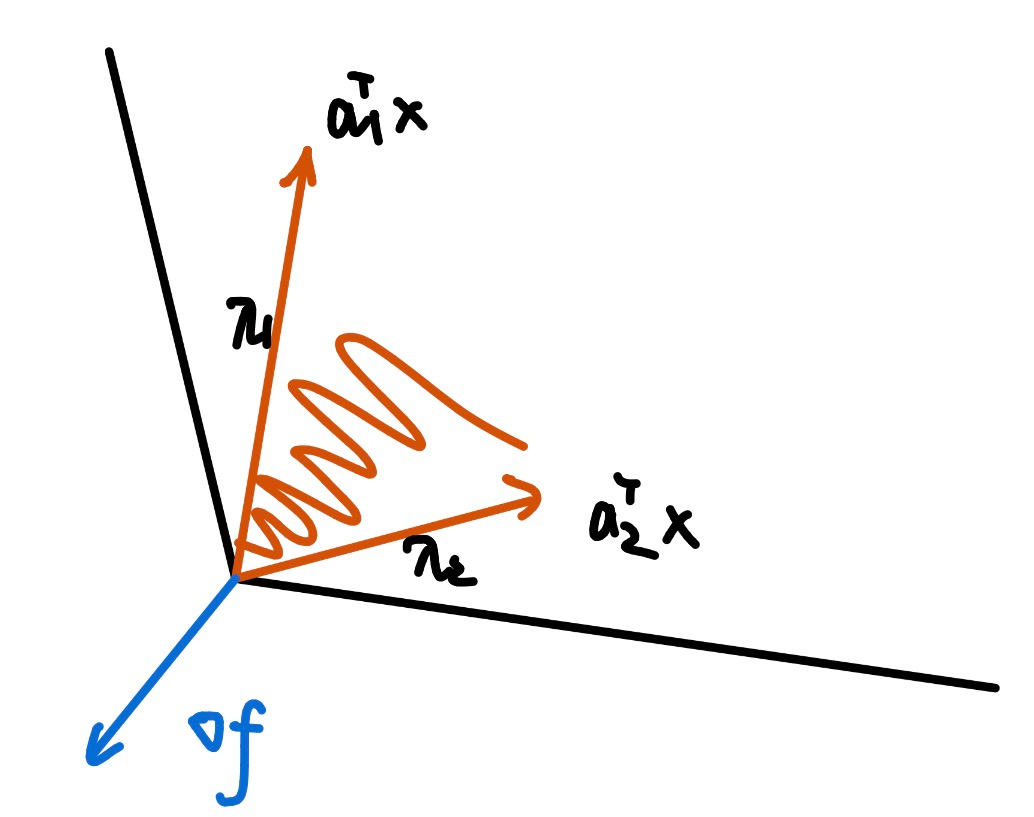
\includegraphics[width=0.3\linewidth]{figures/20260929223822798.png}
\end{center}

另外还有一种理解方式更加物理直观. 所有的可行约束类似一个墙壁 (例如图中的边界). 而墙壁所提供的支持力就是法方向. 故法锥可以理解为所有约束 (墙壁) 所提供的支持力的合力, 而 Lagrange multiplier $\lambda_i$ 就是每个约束所提供的支持力的大小. 因此, 若下降方向处在法锥中, 则说明我们能够通过调整各个墙壁提供的支持力的大小, 来抵消下降方向的作用, 也即我们已经无法继续下降了. 而若一个下降方向不在法锥中, 则说明我们无法通过现有力的合成来抵消下降方向的作用, 因此这将会导致我们继续下降, 也即不是最优解.

\subsection{Convex cones, dual cones, polar cones}

\subsubsection{Cones}


% Source Markdown lines 460–466
\begin{defblock}[{Cones}]
回顾, 定义 $\mathcal{K} \subseteq \mathbb{R}^n$ 是一个 cone, 若: $\lambda \bm{x} \in \mathcal{K},~ \forall \bm{x} \in \mathcal{K},~ \forall \lambda \geq 0$.  进一步, 对于一个锥 $\mathcal{K}$，若其是凸集, 则称之为 convex cone. 也即, 对于任意 $\bm{x}, \bm{y} \in \mathcal{K}$，有 $\lambda \bm{x} + (1-\lambda) \bm{y} \in \mathcal{K},~ \forall \lambda \in [0,1]$.

下面是与 cone 相关的一些概念.

\begin{itemize}
\item {}\emph{Pointed cone}: 若 $\mathcal{K} \cap (-\mathcal{K}) = \{\bm{0}\}$，则称 $\mathcal{K}$ 是 pointed cone. 其中 $-\mathcal{K} := \{-\bm{x}: \bm{x} \in \mathcal{K}\}$. 例如, 非负正交锥 $\mathbb{R}^n_+$ 是 pointed cone, 而 $\mathbb{R}^n$ 不是 pointed cone.


\item {}\emph{Solid cone}: 若 $\mathcal{K}$ 的 interior 非空, 则称 $\mathcal{K}$ 是 solid cone. 例如, 非负正交锥 $\mathbb{R}^n_+$ 是 solid cone, 而 $\mathcal{K} = \{(t,0): t \geq 0\} \subseteq \mathbb{R}^2$ (即一条射线) 不是 solid cone.


\item {}\emph{Proper cone}: 若 $\mathcal{K}$ 是 pointed, closed, convex 且 solid, 则称 $\mathcal{K}$ 是 proper cone.


\end{itemize}

\end{defblock}

\subsubsection{Tangent cone}

\textbf{切锥为可行方向及其极限方向构成的集合.}


% Source Markdown lines 472–475
\begin{defblock}[{Tangent cone}]
给定非空闭凸集 $\mathcal{C} \subseteq \mathbb{R}^n$，定义 $\bm{x} \in \mathcal{C}$ 处的切锥为:

\[
\mathcal{T}_{\mathcal{C}}(\bm{x}) := \text{cl}(\text{cone}(\mathcal{C}-\bm{x})) = \text{cl}\{\lambda(\bm{y}-\bm{x}): \lambda \geq 0,~ \bm{y} \in \mathcal{C}\}.
\]

\end{defblock}

\begin{itemize}
\item {}$\mathcal{C} - \bm{x}$ 表示从 $\bm{x}$ 出发, 指向集合内部的所有点. cone 表示可以在这些方向上进行任意伸缩. 而 closure 则会包含极限点 (如切线方向等)

\begin{itemize}
\item {}例如, 对于单位圆盘 $\mathcal{C} = \{\bm{x} \in \mathbb{R}^2: \|\bm{x}\|_2 \leq 1\}$，在 $\bm{x} = (1,0)$ 处, 方向 $(0,1)$ 是一个切线方向, 我们在定义切锥时希望将其包含在内, 因此需要 closure.


\end{itemize}


\item {}因此切锥可理解为从 $\bm{x}$ 出发, 在一阶意义下, 指向集合内部的所有方向的集合 (包括可行方向及其极限).


\end{itemize}

\subsubsection{Polar cone and dual cone}

\begin{center}
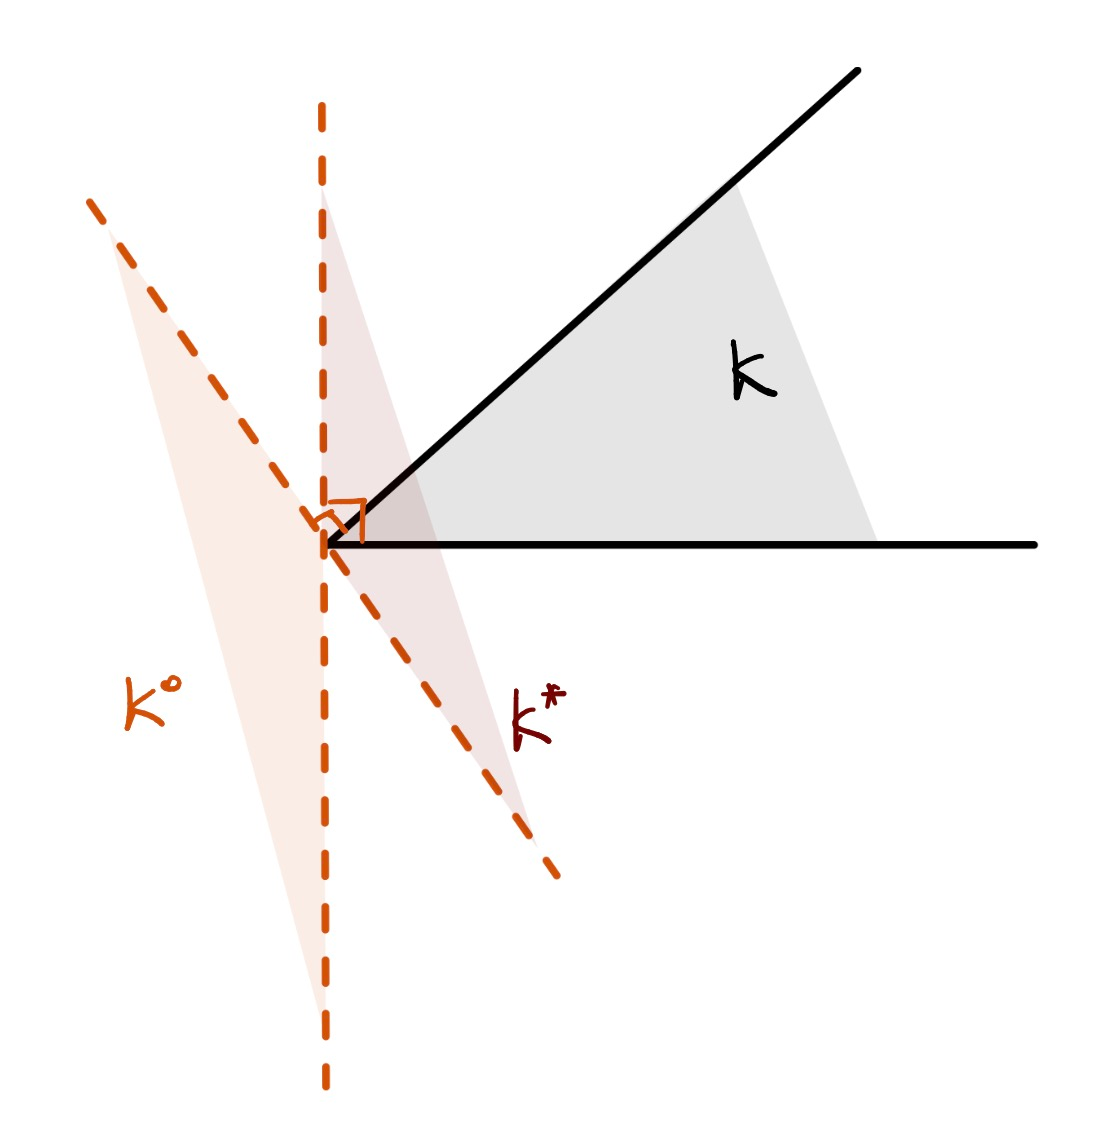
\includegraphics[width=0.4\linewidth]{figures/20261010122849338.png}
\end{center}

\textbf{极锥为与给定集合中所有向量内积非正的向量集合, 即极锥的任意向量与集合中所有向量都呈直角或钝角.}


% Source Markdown lines 486–489
\begin{defblock}[{Polar cone}]
给定非空闭凸集 $\mathcal{C} \subseteq \mathbb{R}^n$，定义 $\mathcal{C}$ 的极锥为:

\[
\mathcal{C}^\circ := \{\bm{v} \in \mathbb{R}^n: \left\langle \bm{v}, \bm{x} \right\rangle \leq 0,~ \forall \bm{x} \in \mathcal{C}\}.
\]

\end{defblock}

\begin{itemize}
\item {}极锥可以理解为所有与集合 $\mathcal{C}$ 中方向不朝向同一侧的向量的集合. 也即, 极锥中的向量与集合 $\mathcal{C}$ 中的所有向量都呈钝角或直角.


\end{itemize}

按此定义, 则有

\[
\mathcal{N}_{\mathcal{C}}(\bm{x}) = \mathcal{T}_{\mathcal{C}}(\bm{x})^\circ,~ \mathcal{T}_{\mathcal{C}}(\bm{x}) = \mathcal{N}_{\mathcal{C}}(\bm{x})^\circ.
\]

\textbf{对偶锥是极锥的反向, 即对偶锥中的向量与集合 $\mathcal{C}$ 中的所有向量都呈锐角或直角.}


% Source Markdown lines 499–502
\begin{defblock}[{Dual cone}]
另外和 polar cone 相关的还有 dual cone 的概念, 定义为:

\[
\mathcal{C}^* := \{\bm{v} \in \mathbb{R}^n: \left\langle \bm{v}, \bm{x} \right\rangle \geq 0,~ \forall \bm{x} \in \mathcal{C}\} = \bigcap_{\bm{x} \in \mathcal{C}} \{\bm{v} \in \mathbb{R}^n: \left\langle \bm{v}, \bm{x} \right\rangle \geq 0\}.
\]

\end{defblock}


% Source Markdown lines 504–509
\begin{propositionblock}[{Dual cone properties}]
对偶锥有如下性质:

\begin{itemize}
\item {}$\mathcal{C}^* = - \mathcal{C}^\circ$.


\item {}$\mathcal{C}^* \cap \mathcal{C}^\circ = \mathcal{C}^\perp$. 极锥和对偶锥的交集是 $\mathcal{C}$ 的正交补. 其中 $\mathcal{C}^\perp := \{\bm{v} \in \mathbb{R}^n: \left\langle \bm{v}, \bm{x} \right\rangle = 0,~ \forall \bm{x} \in \mathcal{C}\}$.


\item {}若 $\mathcal{C}_1 \subseteq \mathcal{C}_2$，则有 $\mathcal{C}_2^* \subseteq \mathcal{C}_1^*$. 包含关系是反向的.  当一个锥变大时, 留给外部的空间就变小了.


\item {}\textbf{对偶锥一定是闭凸锥, 不论原锥是否闭或凸.} 这是因为根据 $\mathcal{C}^*$ 的定义, 对于每个给定的 $\bm{x} \in \mathcal{C}$，集合 $\{\bm{v}: \left\langle \bm{v}, \bm{x} \right\rangle \geq 0\}$ 是一个包含原点的 closed half-space 是闭凸集; 而任意多个闭凸集的交集仍然是闭凸集, 故 $\mathcal{C}^*$ 是闭凸集.


\item {}\textbf{Bipolar theorem}: 对于任意非空闭凸锥 $\mathcal{C}$，有 $(\mathcal{C}^*)^* = \mathcal{C}$.


\end{itemize}

\end{propositionblock}

\subsection{Stability of projection: Non-expansiveness and Pythagorean theorem}

投影也是一种算子/映射, 即 $\Pi_{\mathcal{C}}: \mathbb{R}^n \to \mathcal{C}$. 投影的稳定性是讨论对于输入 $\bm{y}$ 的微小扰动, 投影结果 $\Pi_{\mathcal{C}}(\bm{y})$ 的变化情况.


% Source Markdown lines 515–523
\begin{thmblock}[{Firm non-expansiveness}]
对于非空闭凸集 $\mathcal{C} \subseteq \mathbb{R}^n$，$\forall \bm{y}_1, \bm{y}_2 \in \mathbb{R}^n$，有

\[
\|\Pi_{\mathcal{C}}(\bm{y}_1) - \Pi_{\mathcal{C}}(\bm{y}_2)\|_2^2 \leq 
\langle \Pi_{\mathcal{C}}(\bm{y}_1) - \Pi_{\mathcal{C}}(\bm{y}_2), \bm{y}_1 - \bm{y}_2 \rangle.
\]

Firm non-expansiveness 可以直接推出 Non-expansiveness, 即

\[
\|\Pi_{\mathcal{C}}(\bm{y}_1) - \Pi_{\mathcal{C}}(\bm{y}_2)\|_2 \leq \|\bm{y}_1 - \bm{y}_2\|_2.
\]

\end{thmblock}

\begin{itemize}
\item {}Non-expansiveness (非扩张性): 投影后的点之间的距离不会大于投影前的点之间的距离


\end{itemize}


% Source Markdown lines 527–545
\begin{proof}{}
记 $\bm{p}_1 := \Pi_{\mathcal{C}}(\bm{y}_1)$, $\bm{p}_2 := \Pi_{\mathcal{C}}(\bm{y}_2)$. 由 projection variational inequality, 有对于任意 $\bm{x} \in \mathcal{C}$，有

\[
\begin{aligned}
\langle \bm{y}_1 - \bm{p}_1, \bm{x} - \bm{p}_1 \rangle &\leq 0\,\stackrel{\bm{x}:= \bm{p}_2}{\implies} \langle \bm{y}_1 - \bm{p}_1, \bm{p}_2 - \bm{p}_1 \rangle \leq 0,\\
\langle \bm{y}_2 - \bm{p}_2, \bm{x} - \bm{p}_2 \rangle &\leq 0\,\stackrel{\bm{x}:= \bm{p}_1}{\implies} \langle \bm{y}_2 - \bm{p}_2, \bm{p}_1 - \bm{p}_2 \rangle \leq 0.
\end{aligned}
\]

相加即证 firm non-expansiveness:

\[
\langle \bm{y}_1 - \bm{p}_1 - (\bm{y}_2 - \bm{p}_2), \bm{p}_2 - \bm{p}_1 \rangle \leq 0 \implies \langle \bm{p}_1 - \bm{p}_2, \bm{y}_1 - \bm{y}_2 \rangle \geq \|\bm{p}_1 - \bm{p}_2\|_2^2.
\]

再由 Cauchy-Schwarz inequality, 有

\[
\|\bm{p}_1 - \bm{p}_2\|_2^2 \leq \langle \bm{p}_1 - \bm{p}_2, \bm{y}_1 - \bm{y}_2 \rangle \leq \|\bm{p}_1 - \bm{p}_2\|_2 \cdot \|\bm{y}_1 - \bm{y}_2\|_2 \implies \|\bm{p}_1 - \bm{p}_2\|_2 \leq \|\bm{y}_1 - \bm{y}_2\|_2.
\]

\end{proof}


% Source Markdown lines 547–551
\begin{colblock}[{Pythagorean theorem}]
对于非空闭凸集 $\mathcal{C} \subseteq \mathbb{R}^n$，$\forall \bm{y} \in \mathbb{R}^n$，有

\[
\|\bm{y}-\Pi_{\mathcal{C}}(\bm{y})\|_2^2 + \|\Pi_{\mathcal{C}}(\bm{y}) - \bm{x}\|_2^2 \leq \|\bm{y}-\bm{x}\|_2^2,~ \forall \bm{x} \in \mathcal{C}.
\]

若 $\mathcal{C}$ 是 affine space, 则有等号成立.

\end{colblock}

\subsection{Projection Distance}

前文说到投影是稳定的. 然而, 稳定性是一个零阶条件, 衡量是函数值对于输入扰动的变化幅度. 然而投影算子并不一定是连续可微的. 例如考虑一维空间中 $\mathcal{C} = \mathbb{R}_+$，则 $\Pi_{\mathcal{C}}(x) = \max\{0, x\}$，其在 $x=0$ 处不可微.


% Source Markdown lines 557–560
\begin{defblock}[{Squared projection distance}]
不过, 若考虑点到集合的距离函数, 则其具有更好的性质. 定义平方距离为

\[
\rho_{\mathcal{C}}(\bm{y}) := \frac12 d(\bm{y}, \mathcal{C})^2 = \frac12 \|\bm{y}-\Pi_{\mathcal{C}}(\bm{y})\|_2^2.
\]

\end{defblock}


% Source Markdown lines 562–565
\begin{propositionblock}[{平方投影距离是凸且可微的}]
[Nesterov, § 2.2.3, Lemma 2.2.9; Beck, § 6.7.2, Theorem 6.60; Example 6.61] \emph{(平方投影距离是凸且可微的)}. 给定 $\mathcal{C}$ 是非空闭凸集, 则 $\rho_{\mathcal{C}}(\bm{y})$ 是 convex 且处处可微, 且其梯度是 Lipschitz continuous, 取值为

\[
\nabla \rho_{\mathcal{C}}(\bm{y}) = \bm{y}-\Pi_{\mathcal{C}}(\bm{y}).
\]

\end{propositionblock}


% Source Markdown lines 567–594
\begin{proof}{}
直接通过 Fréchet differentiability 来证明. 给定 $\bm{y}_1 , \bm{y}_2 \in \mathbb{R}^n$，记 $\bm{p}_1 := \Pi_{\mathcal{C}}(\bm{y}_1)$, $\bm{p}_2 := \Pi_{\mathcal{C}}(\bm{y}_2)$. 令 $\bm{d} := \bm{y}_2 - \bm{y}_1$.

首先考虑上界.

\[
\begin{aligned}
\rho_{\mathcal{C}}(\bm{y}_2) &= \frac12 \|\bm{y}_2 - \bm{p}_2\|_2^2 \\&\leq \frac12 \|\bm{y}_2 - \bm{p}_1\|_2^2\qquad {\small(\text{因为 $\bm{p}_2$ 是 $\bm{y}_2$ 的投影, 而 $\bm{p}_1 \in \mathcal{C}$ 是任意可行点})}\\
&= \frac12 \|\bm{y}_1 - \bm{p}_1 + \bm{y}_2 - \bm{y}_1\|_2^2\\
&= \frac12 \|\bm{y}_1 - \bm{p}_1\|_2^2 + \frac12 \|\bm{y}_2 - \bm{y}_1\|_2^2 + \langle \bm{y}_1 - \bm{p}_1, \bm{y}_2 - \bm{y}_1 \rangle\\
&=  \rho_{\mathcal{C}}(\bm{y}_1) + \langle \bm{y}_1 - \bm{p}_1, \bm{d} \rangle + \frac12 \|\bm{d}\|_2^2.
\end{aligned}
\]

其次考虑下界.

\[
\begin{aligned}
  \rho_{\mathcal{C}}(\bm{y}_2) &= \frac12 \|\bm{y}_2 - \bm{p}_2\|_2^2 \\
  &= \frac12 \|\bm{y}_1 - \bm{p}_1 + \left(\bm{y}_2 - \bm{y}_1 + \bm{p}_1 - \bm{p}_2\right)\|_2^2\\
  &= \frac12 \|\bm{y}_1 - \bm{p}_1\|_2^2 + \frac12 \|\bm{d} + \bm{p}_1 - \bm{p}_2\|_2^2 + \langle \bm{y}_1 - \bm{p}_1, \bm{d} \rangle + \underbrace{\langle \bm{y}_1 - \bm{p}_1, \bm{p}_1 - \bm{p}_2 \rangle}_{{\small{\text{Proj. VI.}\geq 0}}}\\
  &\geq \rho_{\mathcal{C}}(\bm{y}_1) + \langle \bm{y}_1 - \bm{p}_1, \bm{d} \rangle .
\end{aligned}
\]

整理上下界, 左右同除 $\|\bm{d}\|_2$ 有

\[
0 \leq \frac{\rho_{\mathcal{C}}(\bm{y}_2) - \rho_{\mathcal{C}}(\bm{y}_1) - \langle \bm{y}_1 - \bm{p}_1, \bm{d} \rangle}{\|\bm{d}\|_2} \leq \frac12 \|\bm{d}\|_2.
\]

令 $\bm{d} \to 0$，故$\rho_{\mathcal{C}}$ 在 $\bm{y}_1$ 处 Fréchet 可微, 其梯度为 $\nabla \rho_{\mathcal{C}}(\bm{y}_1) = \bm{y}_1 - \bm{p}_1$.

\end{proof}


% Source Markdown lines 596–608
\begin{remarkblock}[{Fréchet differentiability}]
回顾: Fréchet differentiability. 在一元函数 $f: \mathbb{R} \to \mathbb{R}$ 中, 若 $f$ 在 $x_0$ 处可微, 则有

\[
f'(x_0) = \lim_{h \to 0} \frac{f(x_0+h)-f(x_0)}{h} \iff f(x_0+h) = f(x_0) + f'(x_0)h + o(|h|), h \to 0.
\]

换言之, 对于输入 $x_0$ 的微小扰动 $h$，函数值的变化可以用线性函数 $f'(x_0)h$ 来近似, 且误差是高阶无穷小.

扩展到多元函数 $f: \mathbb{R}^n \to \mathbb{R}$，此时输入扰动是一个向量 $\bm{d} \in \mathbb{R}^n$，我们同样希望可以用某个线性函数来近似函数值的变化, 且误差是高阶无穷小. 故可微的定义为: 若存在一个线性映射 $L : \mathbb{R}^n \to \mathbb{R}$，使得

\[
\lim_{\bm{d} \to 0} \frac{|f(\bm{x}_0 + \bm{d}) - f(\bm{x}_0) - L(\bm{d})|}{\|\bm{d}\|} = 0 \iff f(\bm{x}_0 + \bm{d}) = f(\bm{x}_0) + L(\bm{d}) + o(\|\bm{d}\|),
\]

则称 $f$ 在 $\bm{x}_0$ 处可微.

特别地, 在 Euclidean space 中, 每个线性映射 $L(\bm{d}): \mathbb{R}^n \to \mathbb{R}$ 都可以唯一地表示为内积的形式, 即 $L(\bm{d}) = \langle \bm{g}, \bm{d} \rangle$，我们称 $\bm{g}$ 为 $f$ 在 $\bm{x}_0$ 处的梯度, 记为 $\nabla f(\bm{x}_0) = \bm{g}$.

\end{remarkblock}

\subsection{Proximal operator and Moreau envelope}


% Source Markdown lines 613–616
\begin{defblock}[{Proximal operator}]
对于 proper closed convex 函数 $f$, proximal operator 是投影算子的一种推广, 其定义为:

\[
\text{prox}_{\gamma f}(\bm{y}) := \arg\min_{\bm{x} \in \mathbb{R}^n} \left\{f(\bm{x}) + \frac{1}{2\gamma}\|\bm{x}-\bm{y}\|_2^2\right\},~ \gamma > 0.
\]

\end{defblock}

\begin{itemize}
\item {}粗略地, proximal operator 尝试在输入点 $\bm{y}$ 附近寻找可以相对最小化 $f$ 的点. 因此这里也天然地引入了距离.


\end{itemize}


% Source Markdown lines 619–622
\begin{defblock}[{Indicator function}]
对于非空闭凸集 $\mathcal{C}$, indicator function $\delta_{\mathcal{C}}(\bm{x})$ 是一个特殊的凸函数, 其定义为:

\[
\delta_{\mathcal{C}}(\bm{x}) := \begin{cases} 0, & \bm{x} \in \mathcal{C}\\ +\infty, & \bm{x} \notin \mathcal{C}\end{cases}.
\]

\end{defblock}

\begin{itemize}
\item {}往往可以将约束优化问题 $\min_{\bm{x} \in \mathcal{C}} f(\bm{x})$ 转化为无约束优化问题 $\min_{\bm{x} \in \mathbb{R}^n} f(\bm{x}) + \delta_{\mathcal{C}}(\bm{x})$, 因为若想要取到最优解, 则 $\bm{x}$ 必须在 $\mathcal{C}$ 中, 否则目标函数值为 $+\infty$.


\end{itemize}

故若考虑 $\text{prox}_{\gamma \delta_{\mathcal{C}}}(\bm{y})$，则有

\[
\text{prox}_{\gamma \delta_{\mathcal{C}}}(\bm{y}) = \arg\min_{\bm{x} \in \mathbb{R}^n} \left\{ \delta_{\mathcal{C}}(\bm{x}) + \frac{1}{2\gamma}\|\bm{x}-\bm{y}\|_2^2 \right\} = \arg\min_{\bm{x} \in \mathcal{C}} \frac{1}{2\gamma}\|\bm{x}-\bm{y}\|_2^2 = \Pi_{\mathcal{C}}(\bm{y}).
\]

\begin{itemize}
\item {}这也是符合 proximal operator 的直观理解的: 若想要最小化 $\delta_{\mathcal{C}}(\bm{x})$，则 $\bm{x}$ 必须在 $\mathcal{C}$ 中; 与此同时又希望找到的点尽量靠近 $\bm{y}$，因此 $\text{prox}_{\gamma \delta_{\mathcal{C}}}(\bm{y})$ 就是 $\bm{y}$ 在 $\mathcal{C}$ 上的投影.


\end{itemize}


% Source Markdown lines 632–635
\begin{defblock}[{Moreau envelope}]
另一个与之相关的重要概念是 Moreau envelope, 其定义为:

\[
M_{\gamma f}(\bm{y}) := \min_{\bm{x} \in \mathbb{R}^n} \left\{f(\bm{x}) + \frac{1}{2\gamma}\|\bm{x}-\bm{y}\|_2^2\right\},~ \gamma > 0.
\]

\end{defblock}

\begin{itemize}
\item {}Proximal operator 是寻找 argmin, 而 Moreau envelope 是寻找对应的最小值函数.


\item {}例如, 若考虑 $M_{\gamma \delta_{\mathcal{C}}}(\bm{y})$，则有

\[
M_{\gamma \delta_{\mathcal{C}}}(\bm{y}) = \min_{\bm{x} \in \mathbb{R}^n} \left\{\delta_{\mathcal{C}}(\bm{x}) + \frac{1}{2\gamma}\|\bm{x}-\bm{y}\|_2^2\right\} = \min_{\bm{x} \in \mathcal{C}} \frac{1}{2\gamma}\|\bm{x}-\bm{y}\|_2^2 = \frac{1}{2\gamma} d(\bm{y}, \mathcal{C})^2.
\]

这也反映了 Moreau envelope 具有光滑化的特性. 对比原始的 $\delta_{\mathcal{C}}(\bm{x})$，其在 $\mathcal{C}$ 内部是平的, 在 $\mathcal{C}$ 外部是无穷大, 其梯度在 $\operatorname{int}(\mathcal{C})$ 内处处为零, 在 $\mathcal{C}$ 外部处处不存在. 而 Moreau envelope 则是一个光滑的函数, 其梯度恰为 $\nabla M_{\gamma \delta_{\mathcal{C}}}(\bm{y}) = \frac{1}{\gamma}(\bm{y}-\Pi_{\mathcal{C}}(\bm{y}))$.


\end{itemize}

\subsection{Examples of projections}


% Source Markdown lines 645–648
\begin{exampleblock}[{Projection onto a halfspace}]
给定半空间 $\mathcal{H} := \{\bm{x} \in \mathbb{R}^n: \bm{a}^\top \bm{x} \leq b\}$，$\bm{a} \neq \bm{0}$，则 $\forall \bm{y} \in \mathbb{R}^n$，有

\[
\Pi_{\mathcal{H}}(\bm{y}) = \begin{cases} \bm{y}, & \text{if } \bm{y} \in \mathcal{H}\\ \bm{y} - \frac{(\bm{a}^\top \bm{y}-b)_+}{\|\bm{a}\|_2^2}\bm{a}, & \text{if } \bm{y} \notin \mathcal{H}\end{cases}.
\]

\end{exampleblock}


% Source Markdown lines 650–654
\begin{proof}{}
$\bm{y} \in \mathcal{H}$ 的情况是显然的. 若 $\bm{y} \notin \mathcal{H}$，实际上这是解析几何的经典公式. 这里作为复习. 最短距离定出现在点到边界的垂线段上, 因此若记投影点为 $\bm{x}_0$ (即垂足), 则 $\bm{y}$ 在其法方向上, 即 $\bm{y} = \bm{x}_0 + \lambda \bm{a}$, $\lambda \in \mathbb{R}$. 此外又知 $\bm{x}_0 \in \partial \mathcal{H}$，即 $\bm{a}^\top \bm{x}_0 = b$. 二者联立, 得 $\lambda = \frac{\bm{a}^\top \bm{y}-b}{\|\bm{a}\|_2^2}$，从而代入可知 $\bm{x}_0 = \bm{y} - \frac{\bm{a}^\top \bm{y}-b}{\|\bm{a}\|_2^2}\bm{a}$.

\begin{center}
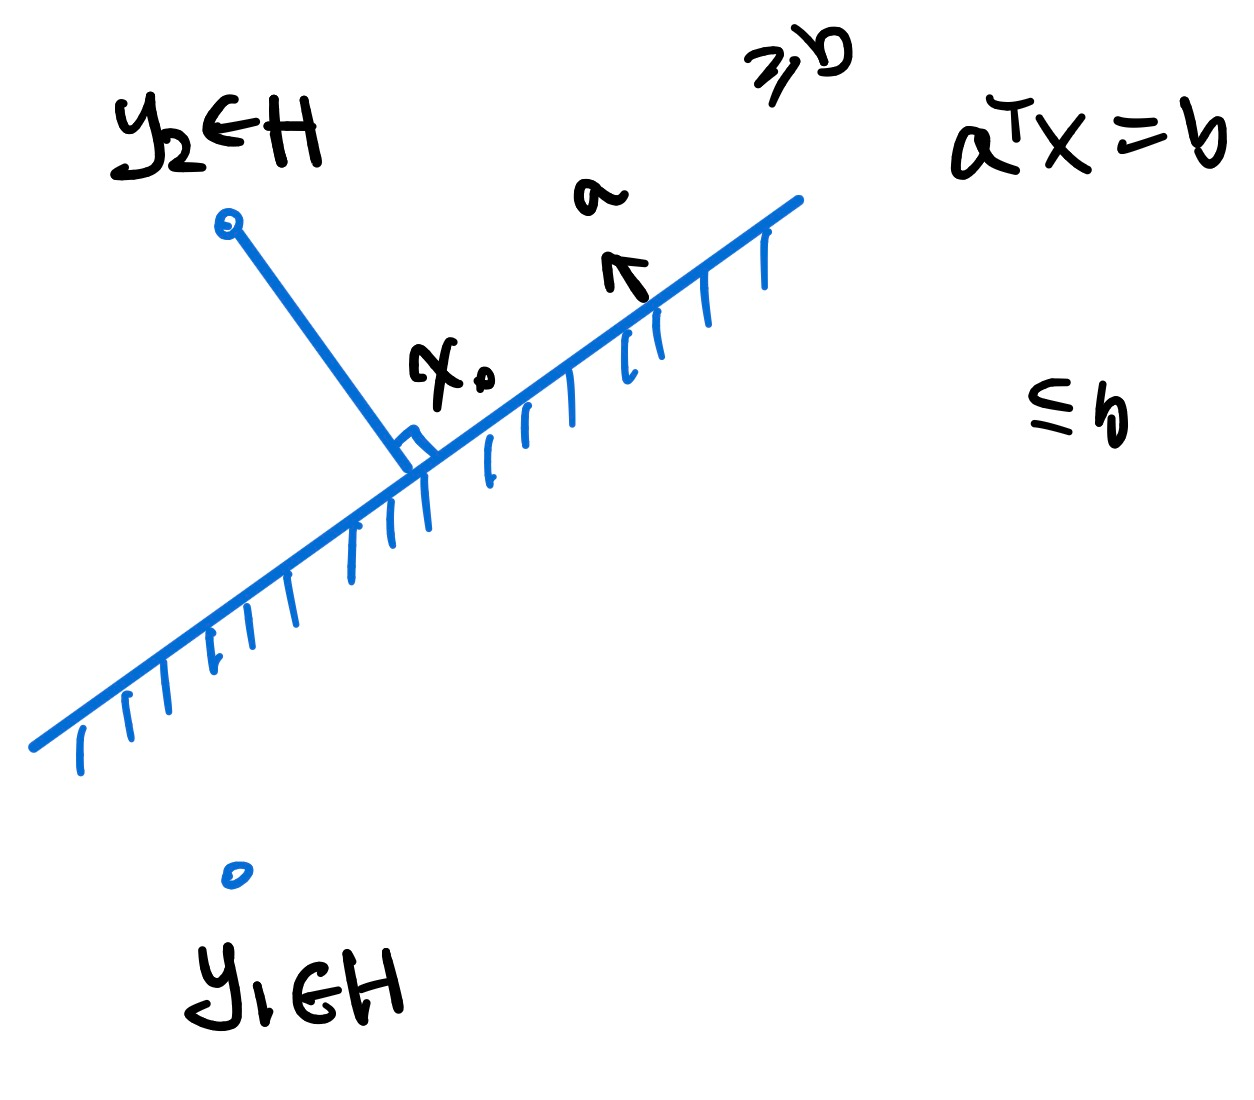
\includegraphics[width=0.3\linewidth]{figures/20261002220459514.png}
\end{center}

\end{proof}


% Source Markdown lines 656–662
\begin{exampleblock}[{Projection onto a non-negative orthant cone}]
定义非负正交锥为 $\mathcal{C} := \mathbb{R}_+^n = \{\bm{x} \in \mathbb{R}^n: x_i \geq 0,~ i=1,\dots,n\}$. 则 $\forall \bm{y} \in \mathbb{R}^n$，有

\[
\Pi_{\mathcal{C}}(\bm{y}) = \max\{\bm{0}, \bm{y}\} = \left(\max\{0, y_1\}, \dots, \max\{0, y_n\}\right)^\top.
\]

即 coordinate-wise ReLU.

\end{exampleblock}


% Source Markdown lines 664–668
\begin{proof}{}
由定义, $\Pi_{\mathcal{C}}(\bm{y}) = \arg\min_{\bm{x} \in \mathcal{C}} \|\bm{x}-\bm{y}\|_2^2 = \arg\min_{\bm{x} \in \mathcal{C}} \sum_{i=1}^n (x_i - y_i)^2$. 由于 $\mathcal{C}$ 是一个正交锥, 故可以 coordinate-wise 分解为 $\arg\min_{x_i \geq 0} (x_i - y_i)^2$, 从而有 $\Pi_{\mathcal{C}}(\bm{y}) = (\max\{0, y_1\}, \dots, \max\{0, y_n\})^\top$.

\begin{quote}
这里有一个重要思想是, 若目标函数和约束集都是 separable 的, 则可以将问题分解为若干个小问题, 分别求解.

\end{quote}

\end{proof}

\section{Separation theorem and supporting hyperplane theorem}

\subsection{Separations}

首先给出 separation 的定义.


% Source Markdown lines 676–681
\begin{defblock}[{Weak and strong separation}]
给定两个非空集合 $\mathcal{S}, \mathcal{T} \subseteq \mathbb{R}^n$，若存在非零向量 $\bm{a} \in \mathbb{R}^n$ 使得

\[
\sup_{\bm{x} \in \mathcal{S}} \bm{a}^\top \bm{x} \leq \inf_{\bm{y} \in \mathcal{T}} \bm{a}^\top \bm{y},
\]

则称 $\mathcal{S}$ 和 $\mathcal{T}$ 是可弱分离的 (weakly separable). 若可以严格取到 $<$，则称 $\mathcal{S}$ 和 $\mathcal{T}$ 是强可分离的 (strongly separable).

\begin{itemize}
\item {}也即, 存在一个超平面 $\mathcal{H}:=\{\bm{z} \in \mathbb{R}^n: \bm{a}^\top \bm{z} = b\}$，使得 $\mathcal{S}$ 和 $\mathcal{T}$ 分别位于该超平面的两侧 (弱分离允许集合接触超平面, 强分离则不允许), 其中 $\sup_{\bm{x} \in \mathcal{S}} \bm{a}^\top \bm{x} \leq b \leq \inf_{\bm{y} \in \mathcal{T}} \bm{a}^\top \bm{y}$.


\end{itemize}

\end{defblock}

\begin{itemize}
\item {}这里再复习/提供一下几何直觉. 给定一个方向 $\bm{a}$，则 $\langle \bm{a}, \bm{x} \rangle$ 可以理解为 $\bm{x}$ 在 $\bm{a}$ 方向上的投影 (这里最好把 $\bm{x}$ 理解为点而不是向量), 也就是 $\bm{x}$ 在 $\bm{a}$ 方向上的坐标. 而固定一个方向 $\bm{a}$，对应超平面就只能在 $\bm{a}$ 方向上下移动. 因此只要两个集合在 $\bm{a}$ 方向上的投影不重叠, 则在二者的 gap 区域取的点都可以确定一个超平面, 使得二者被分开.


\end{itemize}

\begin{center}
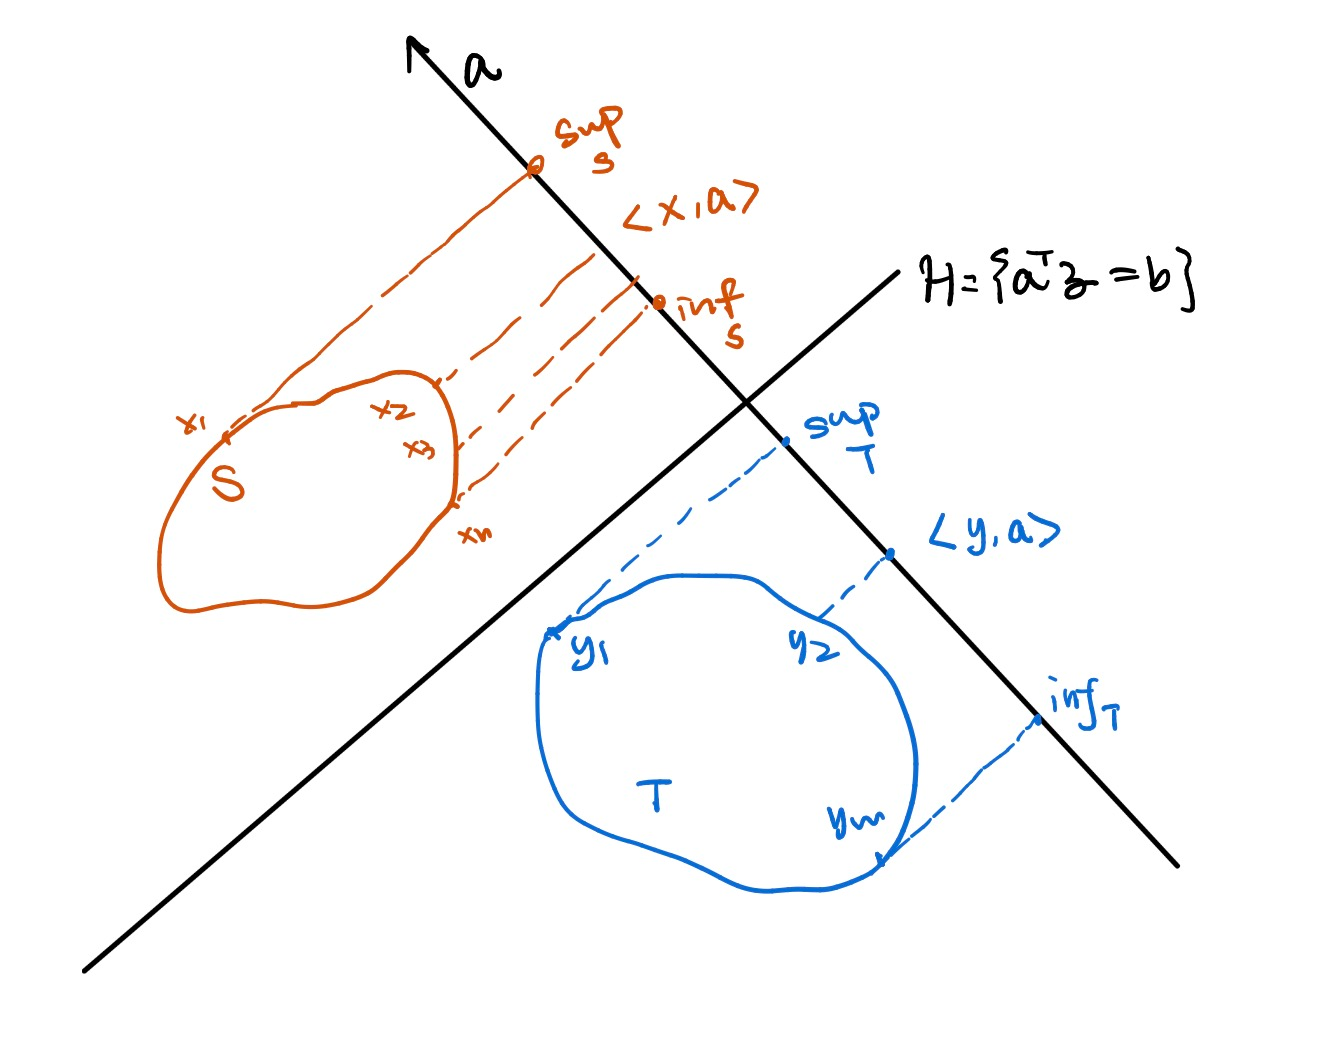
\includegraphics[width=0.6\linewidth]{figures/20261003153442526.png}
\end{center}


% Source Markdown lines 686–691
\begin{defblock}[{Proper separation}]
此外区分 weak separation 和 proper separation. 在 weak separation 中有一个退化情景, 即 $\mathcal{S}$ 和 $\mathcal{T}$ 都完全位于超平面上. 因此在 Ben-Tal-Nemirovski 的书中, 其定义的 separation 是 proper separation, 即要求至少有一个集合不完全位于超平面上. 也即下方定义的第二个条件:

\[
\sup_{\bm{x} \in \mathcal{S}} \bm{a}^\top \bm{x} \leq \inf_{\bm{y} \in \mathcal{T}} \bm{a}^\top \bm{y} \quad \land \quad \inf_{\bm{x} \in \mathcal{S}} \bm{a}^\top \bm{x} < \sup_{\bm{y} \in \mathcal{T}} \bm{a}^\top \bm{y}.
\]

\begin{itemize}
\item {}之所以可以排除退化情况, 是因为根据条件一有: $\inf_{\mathcal{S}} \cdot \leq \sup_{\mathcal{S}} \cdot \leq \inf_{\mathcal{T}} \cdot \leq \sup_{\mathcal{T}} \cdot$. 因此第二个条件可以保证至少有一个 $\leq$ 是严格的 $<$.


\end{itemize}

\end{defblock}

\subsection{Separation theorem}


% Source Markdown lines 697–700
\begin{thmblock}[{Point-set separation}]
[Bertsimas, § 4.7, Theorem 4.11]: 给定 $\mathcal{C} \subseteq \mathbb{R}^n$ 是非空闭凸集, 给定 $\bm{x}^\star \notin \mathcal{C}$，则定存在向量 $\bm{c} \in \mathbb{R}^n$ 使得对于任意 $\bm{x} \in \mathcal{C}$，有

\[
\bm{c}^\top \bm{x} < \bm{c}^\top \bm{x}^\star.
\]

\end{thmblock}

\begin{center}
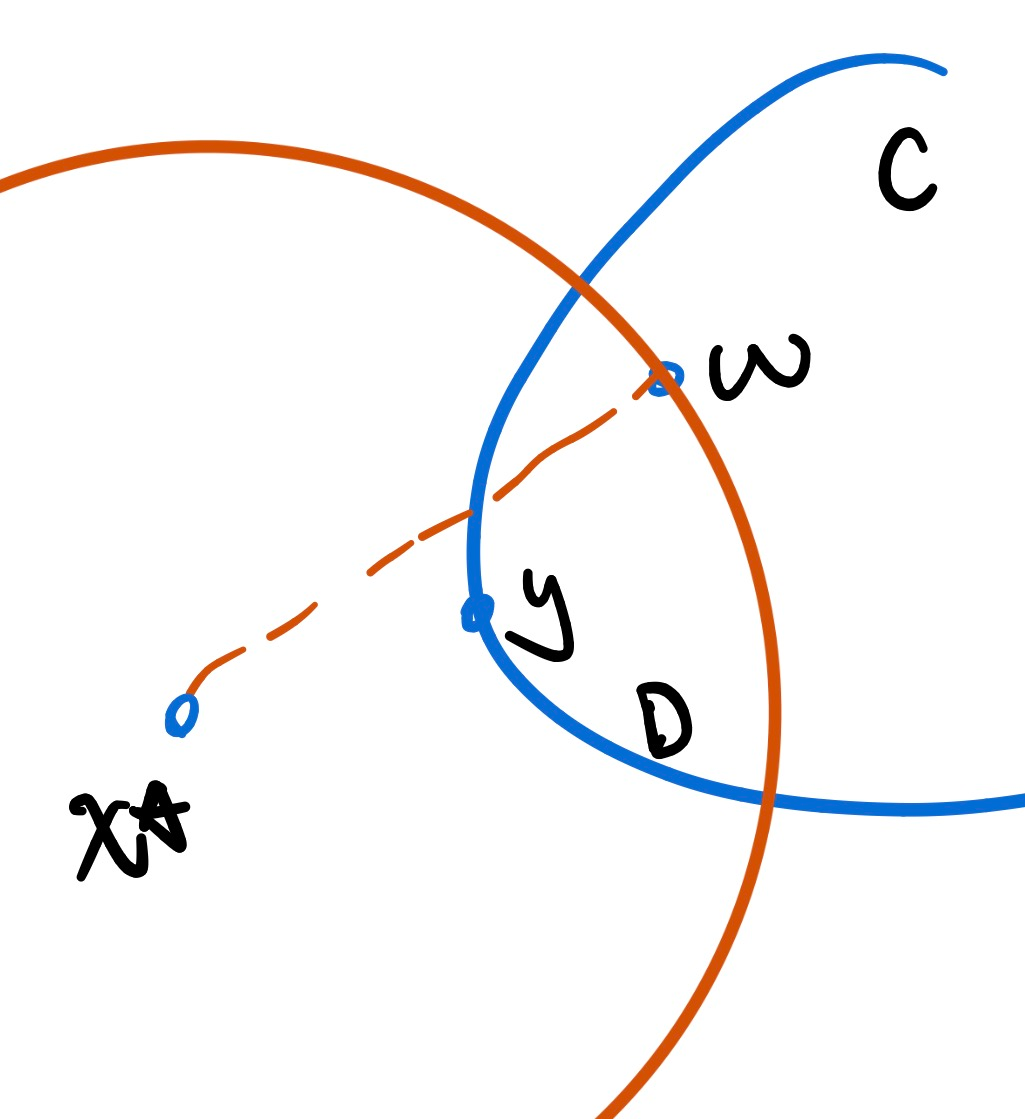
\includegraphics[width=0.3\linewidth]{figures/20261003113803639.png}
\end{center}


% Source Markdown lines 705–732
\begin{proof}{}
原书中的证明过程相当于分别依次证明了如下两个命题, 这两个命题的具体证明细节与前面叙述的基本完全一致, 故不再详细赘述.

\begin{itemize}
\item {}首先利用向闭凸集的投影定理, 记 $\bm{y} := \Pi_{\mathcal{C}}(\bm{x}^\star)$ 为 $\bm{x}^\star$ 在 $\mathcal{C}$ 上的投影点.


\item {}接着, 利用 projection variational inequality, 有

\[
\langle \bm{x}^\star - \bm{y}, \bm{x}- \bm{y} \rangle \leq 0,~ \forall \bm{x} \in \mathcal{C}.
\]

记 $\bm{c} := \bm{x}^\star - \bm{y}$，且 $\bm{c} \neq \bm{0}$，则有

\[
\langle \bm{c}, \bm{x}- \bm{y} \rangle \leq 0,~ \forall \bm{x} \in \mathcal{C} \implies \langle \bm{c}, \bm{x} \rangle \leq \langle \bm{c}, \bm{y} \rangle,~ \forall \bm{x} \in \mathcal{C}.
\]


\item {}另一方面, 考虑

\[
\langle \bm{c}, \bm{x}^\star - \bm{y} \rangle = \langle \bm{x}^\star - \bm{y}, \bm{x}^\star - \bm{y} \rangle = \|\bm{x}^\star - \bm{y}\|_2^2 > 0.
\]

故有 $\langle \bm{c}, \bm{x}^\star - \bm{y} \rangle > 0$，从而有

\[
\langle \bm{c}, \bm{x}^\star\rangle > \langle \bm{c}, \bm{y}\rangle.
\]


\item {}综上得到

\[
\bm{c}^\top \bm{x} < \bm{c}^\top \bm{x}^\star,~ \forall \bm{x} \in \mathcal{C}.
\]


\end{itemize}

\end{proof}

从上述证明过程也可以看出, 从投影点 $\bm{y}$ 指向外部点 $\bm{x}^\star$ 的向量 $\bm{c}$ 就是将点和集合分开的超平面的法向量. 也即, 超平面 $\mathcal{H} := \{\bm{z} \in \mathbb{R}^n: \bm{c}^\top \bm{z} = \bm{c}^\top \bm{y}\}$ 将集合 $\mathcal{C}$ 和点 $\bm{x}^\star$ 分开.


% Source Markdown lines 737–740
\begin{thmblock}[{Finite-dimensional separation}]
[Ben-Tal-Nemirovski, § B.2.6, Theorem B.2.9]: 若 $\mathcal{S}, \mathcal{T} \subseteq \mathbb{R}^n$ 是非空闭凸集, 则 $\mathcal{S}$ 和 $\mathcal{T}$ 是 properly separable 的, 当且仅当

\[
\text{ri}(\mathcal{S}) \cap \text{ri}(\mathcal{T}) = \emptyset.
\]

\end{thmblock}

\begin{quote}
\emph{Note}.

\end{quote}


% Source Markdown lines 745–751
\begin{remarkblock}[{Separation via the difference set}]
在凸分析中, 常用的一个 trick 是将两个集合的分离问题转化为一个集合和一个点的分离问题. 也即, 考虑 $\mathcal{S}$ 与 $\mathcal{T}$ 的差集 $\mathcal{D} := \mathcal{S}-\mathcal{T} := \{\bm{x}-\bm{y}: \bm{x} \in \mathcal{S}, \bm{y} \in \mathcal{T}\}$，则 $\mathcal{D}$ 是非空凸集, 但不一定闭, 且 $0 \in \mathcal{D} \iff \mathcal{S} \cap \mathcal{T} \neq \emptyset$. 且回顾, 若 $\mathcal{S}$ 和 $\mathcal{T}$ 是 properly separable 的, 则存在 $\bm{a} \in \mathbb{R}^n$ 使得

\[
\bm{a}^\top \bm{x} \leq \bm{a}^\top \bm{y},~ \forall \bm{x} \in \mathcal{S},~ \forall \bm{y} \in \mathcal{T} 
\iff
\bm{a}^\top (\bm{x}-\bm{y}) := \bm{a}^\top \bm{d} \leq 0 = \bm{a}^\top \bm{0},~ \forall \bm{d} \in \mathcal{D}.
\]

因此讨论 $\mathcal{S}$ 和 $\mathcal{T}$ 的分离问题等价于讨论 $\mathcal{D}$ 和 $\{0\}$ 的分离问题. 同样, 若存在某 $\bm{d} \in \mathcal{D}$ 使得 $\bm{a}^\top \bm{d} < 0$ 严格成立, 则说明 $\mathcal{S}$ 和 $\mathcal{T}$ 是 properly separable 的. 进一步, 若 $\sup_{\bm{d} \in \mathcal{D}} \bm{a}^\top \bm{d} < 0$，则说明 $\sup_{\bm{x} \in \mathcal{S}} \bm{a}^\top \bm{x} < \inf_{\bm{y} \in \mathcal{T}} \bm{a}^\top \bm{y}$，也即 $\mathcal{S}$ 和 $\mathcal{T}$ 是 strongly separable 的.

\end{remarkblock}


% Source Markdown lines 753–763
\begin{proof}[{Proof Sketch}]
\textbf{(Necessity)}. 即假设 $\mathcal{S}$ 和 $\mathcal{T}$ 是 properly separable 的, 即存在 $\bm{a} \in \mathbb{R}^n$ 使得

\[
\sup_{\bm{x} \in \mathcal{S}} \bm{a}^\top \bm{x} \leq \inf_{\bm{y} \in \mathcal{T}} \bm{a}^\top \bm{y} \quad \land \quad \inf_{\bm{x} \in \mathcal{S}} \bm{a}^\top \bm{x} < \sup_{\bm{y} \in \mathcal{T}} \bm{a}^\top \bm{y}.
\]

则不可能存在 $\bm{z} \in \text{ri}(\mathcal{S}) \cap \text{ri}(\mathcal{T})$. 由反证法, 若不然, 则由于 $\bm{z} \in \text{ri}(\mathcal{S})$，且 $\bm{z} \in \text{ri}(\mathcal{T})$，故有 $\bm{a}^\top \bm{z} \leq \sup_{\bm{x} \in \mathcal{S}} \bm{a}^\top \bm{x} \leq \inf_{\bm{y} \in \mathcal{T}} \bm{a}^\top \bm{y} \leq \bm{a}^\top \bm{z}$，从而 $\bm{a}^\top \bm{z} = \sup_{\bm{x} \in \mathcal{S}} \bm{a}^\top \bm{x} = \inf_{\bm{y} \in \mathcal{T}} \bm{a}^\top \bm{y}$. 然而有引理: \emph{若线性目标函数 $\bm{a}^\top \bm{x}$ 在凸集 $\mathcal{C}$ 的内部 $\text{ri}(\mathcal{C})$ 上取得最优值, 则该目标函数在 $\mathcal{C}$ 上必为常函数.} 而这与 proper 的定义矛盾, 因此 $\text{ri}(\mathcal{S}) \cap \text{ri}(\mathcal{T}) = \emptyset$.

\textbf{(Sufficiency)}. 即假设 $\text{ri}(\mathcal{S}) \cap \text{ri}(\mathcal{T}) = \emptyset$，则 $\mathcal{S}$ 和 $\mathcal{T}$ 是 properly separable 的. 这里有两个事实: \emph{对于非空凸集 $\mathcal{S}$ 和 $\mathcal{T}$，$\text{ri}(\mathcal{S})$ 与 $\text{ri}(\mathcal{T})$ 非空且凸的}, 且 $\text{cl}(\text{ri}(\mathcal{S})) = \text{cl}(\mathcal{S})$, $\text{cl}(\text{ri}(\mathcal{T})) = \text{cl}(\mathcal{T})$. 对于非空凸集 $\text{ri}(\mathcal{S})$ 和 $\text{ri}(\mathcal{T})$，由于二者不交, 故定存在 $\bm{a} \neq \bm{0}$ 分离二者且是 proper 的. 再根据 $\text{cl}(\text{ri}(\mathcal{S})) = \text{cl}(\mathcal{S})$, $\text{cl}(\text{ri}(\mathcal{T})) = \text{cl}(\mathcal{T})$，以及函数 $\bm{a}^\top \bm{x}$ 的连续性, 因此 $\sup_{\bm{x} \in \text{ri}(\mathcal{S})} \bm{a}^\top \bm{x} = \sup_{\bm{x} \in \mathcal{S}} \bm{a}^\top \bm{x}$, $\inf_{\bm{y} \in \text{ri}(\mathcal{T})} \bm{a}^\top \bm{y} = \inf_{\bm{y} \in \mathcal{T}} \bm{a}^\top \bm{y}$, 从而扩展到 $\mathcal{S}$ 和 $\mathcal{T}$ 上, 即 $\mathcal{S}$ 和 $\mathcal{T}$ 是 properly separable 的.

\end{proof}


% Source Markdown lines 765–768
\begin{colblock}{}
[Nesterov, § 3.1.4]

\begin{itemize}
\item {}$\mathcal{S}$ 和 $\mathcal{T}$ 是 strongly separable 的, 当且仅当 $\text{dist}(\mathcal{S}, \mathcal{T}) > 0$.


\item {}特别地, 若 $\mathcal{S}, \mathcal{T}$ 是非空闭凸集, $\mathcal{S} \cap \mathcal{T} = \emptyset$，且至少有一个集合是 bounded 的 (即是 compact 的), 则二者是 strongly separable 的.


\item {}若记 $\bm{s}^\star \in \mathcal{S}$ 和 $\bm{t}^\star \in \mathcal{T}$ 为二者的最短距离点, 则 $\bm{s}^\star$ 和 $\bm{t}^\star$ 不一定唯一, 但差向量 $\bm{t}^\star-\bm{s}^\star$ 是唯一的, 且 $\bm{a} := \bm{t}^\star - \bm{s}^\star$ 就是将二者分开的超平面的法向量.


\end{itemize}

\end{colblock}

\subsection{Supporting hyperplane theorem}


% Source Markdown lines 772–780
\begin{defblock}[{Supporting hyperplane}]
在上面的分离定理中的分离超平面中, 恰好经过集合的边界点的, 即为支持超平面 (supporting hyperplane). 具体定义为: 给定非空凸集 $\mathcal{C} \subseteq \mathbb{R}^n$，及边界点 $\bm{x}^\star \in \text{bd}(\mathcal{C})$，若超平面

\[
\mathcal{H} := \{\bm{x} \in \mathbb{R}^n: \bm{a}^\top \bm{x} =  \bm{a}^\top \bm{x}^\star\},~ \bm{a} \neq \bm{0}
\]

满足

\[
\bm{a}^\top \bm{x} \leq \bm{a}^\top \bm{x}^\star,~ \forall \bm{x} \in \mathcal{C},
\]

则称 $\mathcal{H}$ 是在 $\bm{x}^\star$ 处的 supporting hyperplane.

\end{defblock}

\begin{itemize}
\item {}注意, 根据 Boyd-Vandenberghe 的定义, 这里并不要求 $\mathcal{C}$ 是闭集等.


\end{itemize}


% Source Markdown lines 784–784
\begin{thmblock}[{Supporting hyperplane theorem}]
若 $\mathcal{C} \subseteq \mathbb{R}^n$ 是凸集, 则在任意边界点 $\bm{x}^\star \in \text{bd}(\mathcal{C})$ 处, 都存在一个 supporting hyperplane.

\end{thmblock}


% Source Markdown lines 786–786
\begin{proof*}[{Proof Sketch}]
整体证明思路如下. 首先考虑闭凸集, 存在外部点列 $\{\bm{y}_k\} \subseteq \mathbb{R}^n \setminus \mathcal{C}$ 收敛到 $\bm{x}^\star$. 对于外部的每一个点, 根据点与集合的分离定理, 都存在一个分离超平面, 对应着一列法向量 $\{\bm{a}_k\}$. 将法向量归一化后, 序列位于紧的单位球面上, 因此根据 Bolzano-Weierstrass 定理可以选取一个收敛子列 $\{\bm{a}_{k_j}\}$ 收敛到某个 $\bm{a}^\star \neq \bm{0}$. 再根据连续性, 取极限后就可以得到在 $\bm{x}^\star$ 处的 supporting hyperplane.

\end{proof*}


% Source Markdown lines 788–804
\begin{proof*}[{Proof}]
首先考虑 $\mathcal{C}$ 是闭凸集.

\begin{itemize}
\item {}\textbf{Step 1}. 由于 $\bm{x}^\star \in \text{bd}(\mathcal{C})$，则存在 $\{\bm{y}_k\} \subseteq \mathbb{R}^n \setminus \mathcal{C}$ 收敛到 $\bm{x}^\star$. 这是由边界点的定义直接得到的. 也即, 对于任意 $\epsilon > 0$，存在 $\bm{y} \in \mathbb{R}^n \setminus \mathcal{C}$，使得 $\|\bm{y}-\bm{x}^\star\|_2 < \epsilon$. 因此, 对于任意 $k \in \mathbb{N}$，取 $\epsilon = 1/k$，则存在 $\bm{y}_k \in \mathbb{R}^n \setminus \mathcal{C}$，使得 $\|\bm{y}_k - \bm{x}^\star\|_2 < 1/k$，从而 $\bm{y}_k \to \bm{x}^\star$.


\item {}\textbf{Step 2}. 对于每一个 $\bm{y}_k \in \mathbb{R}^n \setminus \mathcal{C}$，根据点与集合的分离定理, 存在 $\bm{a}_k \neq \bm{0}$ 使得

\[
\bm{a}_k^\top \bm{x} < \bm{a}_k^\top \bm{y}_k,~ \forall \bm{x} \in \mathcal{C}.
\]

不妨将 $\bm{a}_k$ 归一化, 即 $\|\bm{a}_k\|_2 = 1$. 则此时, 所有的 $\bm{a}_k$ 都位于单位球面上, 因此 $\{\bm{a}_k\}$ 是有界的, 故定存在收敛子列 $\{\bm{a}_{k_j}\}$ 收敛到某个 $\bm{a}^\star \neq \bm{0}$.


\item {}\textbf{Step 3}. 由前述构造, 已有 $\bm{a}_{k_j}^\top (\bm{x} - \bm{y}_{k_j}) < 0,~ \forall \bm{x} \in \mathcal{C}$. 取极限 $j \to \infty$，得到

\[
\bm{a}^\star{}^\top (\bm{x} - \bm{x}^\star) \leq 0,~ \forall \bm{x} \in \mathcal{C}.
\]

故有 $\bm{a}^\star{}^\top \bm{x} \leq \bm{a}^\star{}^\top \bm{x}^\star,~ \forall \bm{x} \in \mathcal{C}$，从而得到在 $\bm{x}^\star$ 处的 supporting hyperplane.


\end{itemize}

若 $\mathcal{C}$ 不是闭集, 则考虑 $\text{cl}(\mathcal{C})$，此时 $\bm{x}^\star \in \text{bd}(\text{cl}(\mathcal{C}))$，且 $\text{cl}(\mathcal{C})$ 是闭凸集.而 $\mathcal{C} \subseteq \text{cl}(\mathcal{C})$，因此在 $\bm{x}^\star$ 处的 supporting hyperplane 同样是 $\mathcal{C}$ 的 supporting hyperplane.

\end{proof*}


% Source Markdown lines 806–806
\begin{colblock}{}
任意非空闭凸集 $\mathcal{C}$ 都可以表示为所有包含它的 supporting halfspace 的交集.

\end{colblock}

\subsection{Support function and Exposed face}

\emph{\textbf{Support function}}.

回顾, 对于凸集 $\mathcal{C}$, 如果存在 $\bm{a} \neq \bm{0}$ 使得 $\bm{a}^\top (\bm{x}-\bm{x}^\star) \leq 0,~ \forall \bm{x} \in \mathcal{C}$，则称 $\bm{a}$ 是在 $\bm{x}^\star$ 处的 supporting hyperplane 的法向量. 根据这个定义, 超平面本身也意味着:

\[
\bm{a}^\top \bm{x}^\star = \max_{\bm{x} \in \mathcal{C}} \bm{a}^\top \bm{x}.
\]

\begin{itemize}
\item {}可以想象, 每给定一个方向, 就好像有这个方向一个竹签, 有一个横着的面包片可以在竹签上滑动. 竹签上有一个肉丸, 最远能把这个面包片推到多远, 就是这个方向的 support function 的值.


\end{itemize}

\begin{center}
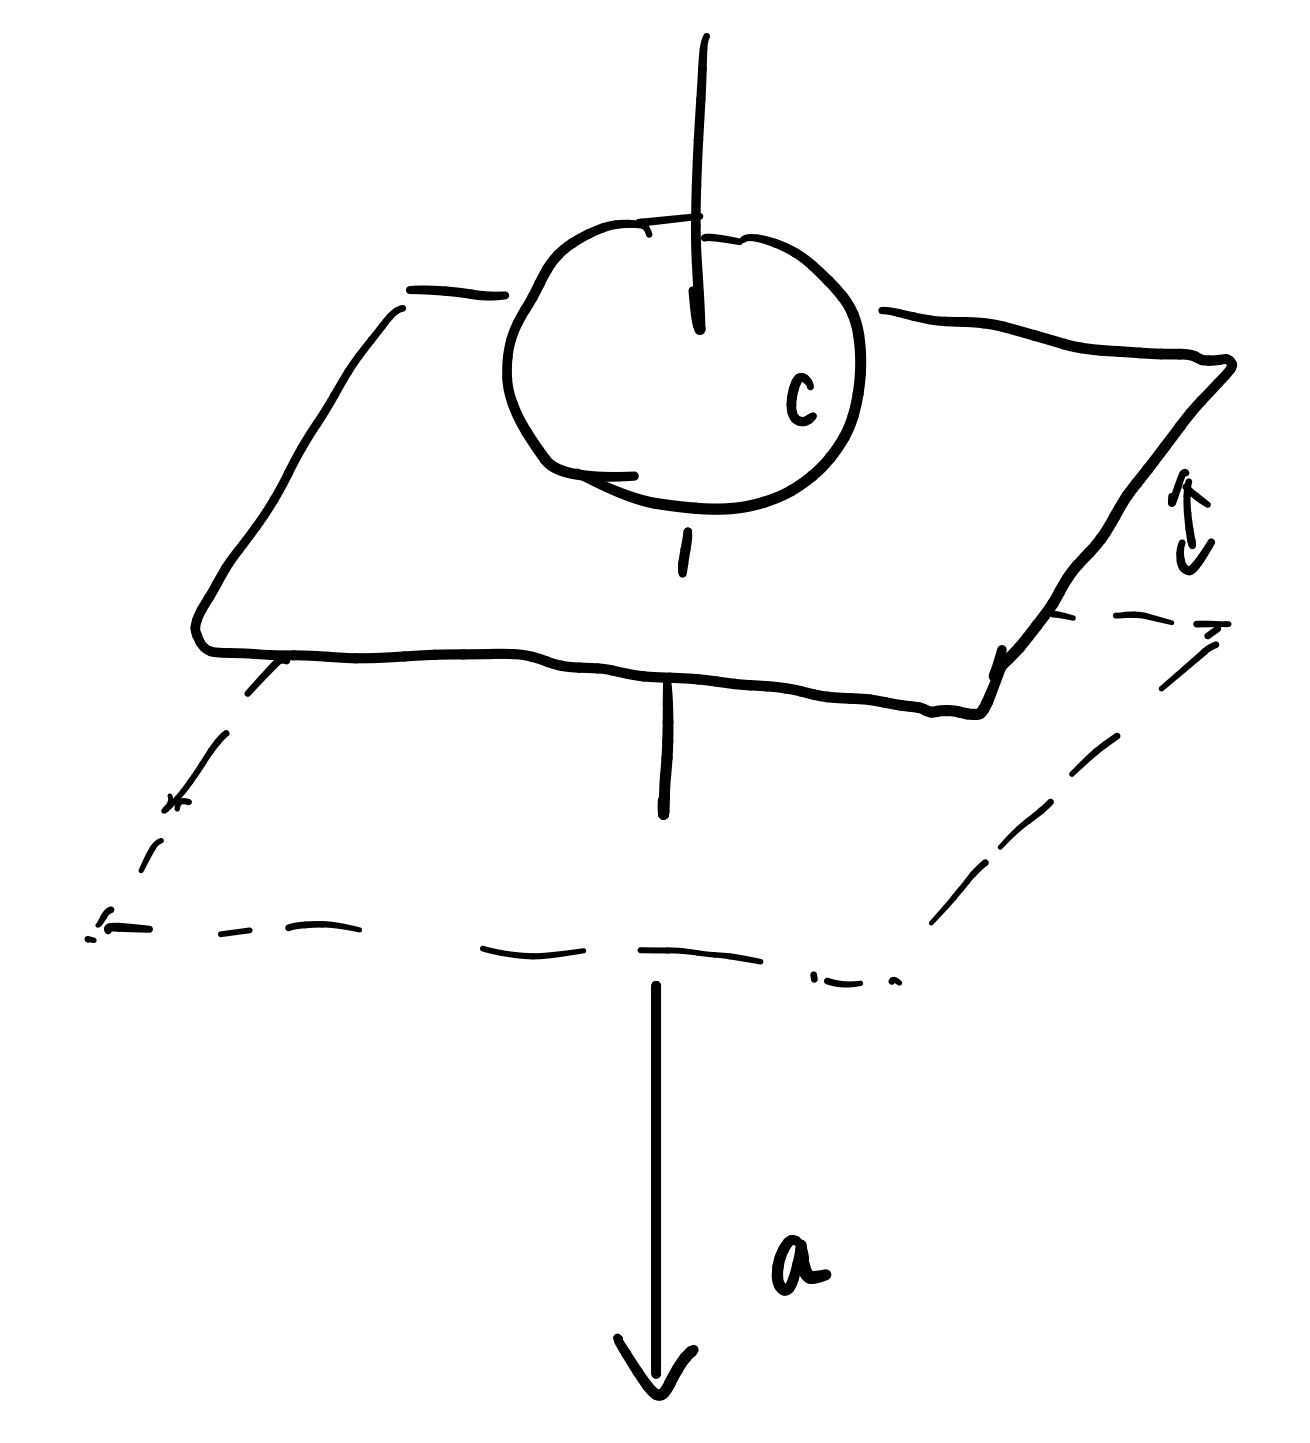
\includegraphics[width=0.3\linewidth]{figures/20261008201613697.png}
\end{center}


% Source Markdown lines 819–823
\begin{defblock}[{Support function}]
对于非空集合 $\mathcal{C} \subseteq \mathbb{R}^n$，定义其 support function 为:

\[
\sigma_{\mathcal{C}}(\bm{a}) := \sup_{\bm{x} \in \mathcal{C}} \bm{a}^\top \bm{x},
\]

\end{defblock}

\begin{itemize}
\item {}当上确界有限且在 $\mathcal{C}$ 中取得时, supporting hyperplane 可以定义为:

\[
\mathcal{H} = \{\bm{x} \in \mathbb{R}^n: \bm{a}^\top \bm{x} = \sigma_{\mathcal{C}}(\bm{a})\},~ \bm{a} \neq \bm{0}.
\]


\end{itemize}


% Source Markdown lines 828–832
\begin{propositionblock}[{Support function representation}]
\begin{itemize}
\item {}前文提到, 一个非空闭凸集 $\mathcal{C}$ 可以表示为所有包含它的 supporting halfspace 的交集, 因此也可以通过 support function 来表示 $\mathcal{C}$:

\[
\mathcal{C} = \bigcap_{\bm{a} \in \mathbb{R}^n \setminus \{\bm{0}\}} \{\bm{x} \in \mathbb{R}^n: \bm{a}^\top \bm{x} \leq \sigma_{\mathcal{C}}(\bm{a})\}.
\]


\end{itemize}

\end{propositionblock}

并且可以由此推论集合之间的包含关系: 对于闭凸集 $\mathcal{C}_1, \mathcal{C}_2 \subseteq \mathbb{R}^n$，有 $\mathcal{C}_1 \subseteq \mathcal{C}_2 \iff \sigma_{\mathcal{C}_1}(\bm{a}) \leq \sigma_{\mathcal{C}_2}(\bm{a}),~ \forall \bm{a} \in \mathbb{R}^n$.


% Source Markdown lines 834–841
\begin{exampleblock}[{Support functions}]
下面是一些常见集合的 support function 的例子:

\begin{itemize}
\item {}对于 Euclidean ball $\mathcal{B}(\bm{c}, r) := \{\bm{x} \in \mathbb{R}^n: \|\bm{x}-\bm{c}\|_2 \leq r\}$，有 $\sigma_{\mathcal{B}(\bm{c}, r)}(\bm{a}) = \bm{a}^\top \bm{c} + r\|\bm{a}\|_2$. 直观上, 可以理解为, 球在方向 $\bm{a}$ 上的评分, 就是由球心 $\bm{c}$ 在方向 $\bm{a}$ 上的投影, 再加上半径 $r$ 在方向 $\bm{a}$ 上的投影 (即 $r\|\bm{a}\|_2$).


\item {}对于 simplex $\Delta_{n-1} := \{\bm{x} \in \mathbb{R}^n: x_i \geq 0,~ \sum_{i=1}^n x_i = 1\}$，有 $\sigma_{\Delta_{n-1}}(\bm{a}) = \max_{i=1,\dots,n} a_i$.
对于三维欧氏空间, simplex 即为由 $(1,0,0), (0,1,0), (0,0,1)$ 三个点构成的等边三角形和内部. 直观上, 可以理解为, simplex 在方向 $\bm{a}$ 上的评分, 就是由三个顶点在方向 $\bm{a}$ 上的投影中最大的那个.
\begin{center}
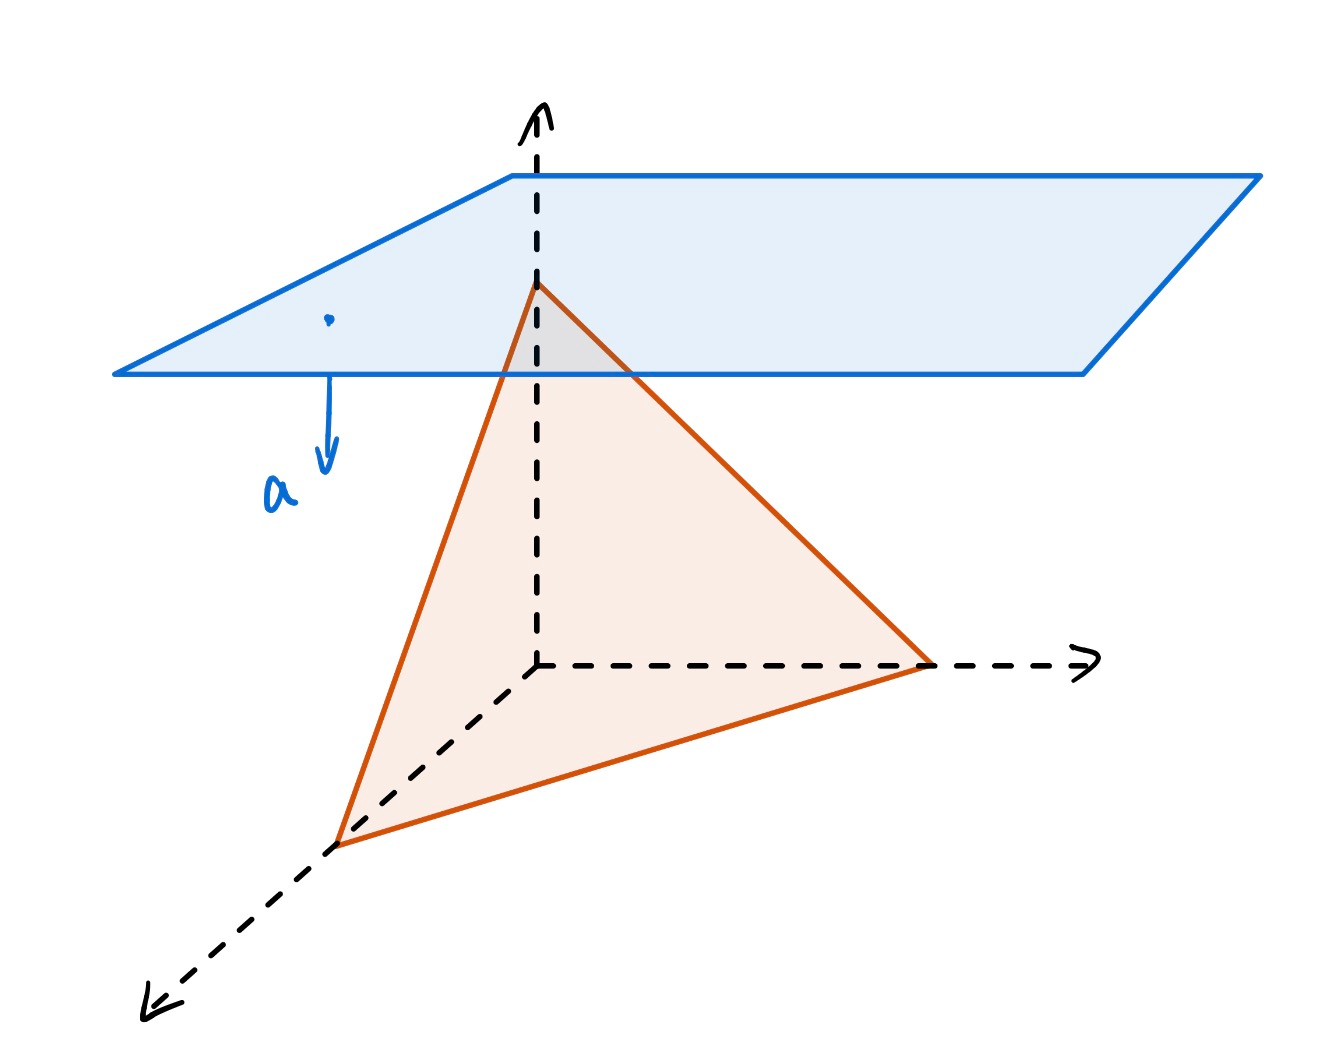
\includegraphics[width=0.4\linewidth]{figures/20261008224136252.png}
\end{center}




\item {}对于 box-constraint set $[l,u]$, 有 $\sigma_{[l,u]}(\bm{a}) = \sum_{i=1}^n \max\{a_i l_i, a_i u_i\}$.


\item {}对于 closed convex cone $\mathcal{K}$, 有 $\sigma_{\mathcal{K}}(\bm{a}) = \delta_{\mathcal{K}^\circ}(\bm{a})$，其中 $\mathcal{K}^\circ$ 是 $\mathcal{K}$ 的极锥 (polar cone).


\end{itemize}

\end{exampleblock}


% Source Markdown lines 843–848
\begin{defblock}[{Exposed face}]
有了集合 $\mathcal{C}$ 和 supporting hyperplane $\mathcal{H}$，exposed face 就是二者的交界面, 即 $\mathcal{F}_{\mathcal{C}}(\bm{a}) := \mathcal{C} \cap \mathcal{H}$. 或者, 也可以直接定义 exposed face 为:

\[
\mathcal{F}_{\mathcal{C}}(\bm{a}) := \arg\max_{\bm{x} \in \mathcal{C}} \bm{a}^\top \bm{x},~ \bm{a} \neq \bm{0}.
\]

\end{defblock}

\emph{\textbf{Deeper view of support function}}.

以上两个数学量的定义本身是直观的. 然而其可以通过凸分析的工具进行更深刻的理解.

首先, support function 可以看作是集合的 indicator function 的 Fenchel conjugate. 理由如下.

\begin{itemize}
\item {}对于 $\sigma_{\mathcal{C}}(\bm{a}) = \sup_{\bm{x} \in \mathcal{C}} \bm{a}^\top \bm{x}$，其关注的是, 给定一个方向 $\bm{a}$，在这个方向上, 集合 $\mathcal{C}$ 能够测量的最大评分是多少.

\begin{itemize}
\item {}例如, 对于 Euclidean ball $\mathcal{C} = \{\bm{x} \in \mathbb{R}^n: \|\bm{x}\|_2 \leq 1\}$，则由 Cauchy-Schwarz inequality 可知 $\bm{a}^\top \bm{x} \leq \|\bm{a}\|_2 \|\bm{x}\|_2 \leq \|\bm{a}\|_2$，故 $\sigma_{\mathcal{C}}(\bm{a}) = \|\bm{a}\|_2$.


\item {}这里从集合 $\mathcal{C}$ 转换成了一个函数 $\sigma_{\mathcal{C}}(\cdot)$.


\end{itemize}


\item {}联想到 Fenchel conjugate. 对于函数 $f: \mathbb{R}^n \to \mathbb{R} \cup \{+\infty\}$，其 Fenchel conjugate 定义为 $f^*(\bm{y}) := \sup_{\bm{x} \in \mathbb{R}^n} \{\bm{y}^\top \bm{x} - f(\bm{x})\}$.

\begin{itemize}
\item {}Fenchel conjugate 关注的是, 在整个 $\mathbb{R}^n$ 空间中的最大化, 但是要扣除一个 penalty $f(\bm{x})$. 而 support function 关注的是, 在集合 $\mathcal{C}$ 中的最大化.


\item {}不妨通过令 $f(\bm{x}) = \delta_{\mathcal{C}}(\bm{x})$，则有 $f^*(\bm{y}) = \sup_{\bm{x} \in \mathbb{R}^n} \{\bm{y}^\top \bm{x} - \delta_{\mathcal{C}}(\bm{x})\} = \sup_{\bm{x} \in \mathcal{C}} \bm{y}^\top \bm{x} = \sigma_{\mathcal{C}}(\bm{y})$. 也即, support function 可以看作是 indicator function 的 Fenchel conjugate.


\end{itemize}


\item {}因此, 集合 $\mathcal{C}$ 的 support function 可以看作是 $\mathcal{C}$ 的 indicator function 的 Fenchel conjugate.


\end{itemize}

\section{Farkas lemma}

\subsection{Standard form}

Farkas lemma 给出了线性系统的可行性的一个判断条件. 其有多种等价的表述. 首先考虑其标准形式.


% Source Markdown lines 871–873
\begin{thmblock}[{Farkas lemma, standard form}]
[Bertsimas, § 4.6, Theorem 4.6]  给定 $\bm{A} \in \mathbb{R}^{m \times n}$, $\bm{x} \in \mathbb{R}^n$，$\bm{b} \in \mathbb{R}^m$，则如下两个命题有且仅有一个成立:

\begin{enumerate}
\item {}存在 $\bm{x} \geq \bm{0}$ 使得 $\bm{A}\bm{x} = \bm{b}$.


\item {}存在 $\bm{y} \in \mathbb{R}^m$ 使得 $\bm{y}^\top \bm{A} \geq \bm{0}^\top$ 且 $\bm{y}^\top \bm{b} < 0$.


\end{enumerate}

\end{thmblock}


% Source Markdown lines 875–887
\begin{proof}{}
记第一个命题为 $P$, 第二个命题为 $Q$. 故该命题要证明的是 $\neg P \iff Q$.

\begin{itemize}
\item {}($Q \Rightarrow \neg P$) 这个方向的证明是比较直接的. 考虑其等价逆否命题, 即存在 $\bm{x} \geq \bm{0}$ 使得 $\bm{A}\bm{x} = \bm{b}$，则此时对于任意 $\bm{y} \in \mathbb{R}^m$，有 $\bm{y}^\top \bm{A}\bm{x} = \bm{y}^\top \bm{b}$. 故若 $\bm{y}^\top \bm{A} \geq \bm{0}^\top$，则有 $\bm{y}^\top \bm{b} = \bm{y}^\top \bm{A}\bm{x} \geq 0$, 从而与 $\bm{y}^\top \bm{b} < 0$ 矛盾.


\item {}($\neg P \Rightarrow Q$) 这个方向的证明是比较复杂的. Bertsimas 的书中是通过如下 LP 问题与其对偶问题的可行性来证明的. 具体而言, 考虑如下 LP 问题:

\[
\min \bm{0}^\top \bm{x} \quad \text{s.t.}~ \bm{A}\bm{x} = \bm{b},~ \bm{x} \geq \bm{0}.
\]

其对偶问题经变量取负后的等价形式为:

\[
\min \bm{b}^\top \bm{y} \quad \text{s.t.}~ \bm{y}^\top \bm{A} \geq \bm{0}^\top.
\]

如果 $\neg P$ 成立, 则说明原问题不可行, 则根据 LP 的对偶性质, 说明对偶问题要么是不可行的, 要么是无界的. 然而显然 $\bm{y} = \bm{0}$ 是对偶问题的一个可行解, 因此只能是对偶问题是无界的, 即 $\bm{b}^\top \bm{y} < 0$ (故最小化时是无界的). 因此, 存在 $\bm{y} \in \mathbb{R}^m$ 使得 $\bm{y}^\top \bm{A} \geq \bm{0}^\top$ 且 $\bm{y}^\top \bm{b} < 0$. 故 $Q$ 成立.


\end{itemize}

\end{proof}

这是一个很简洁的证明视角, 不过其证明依赖于 LP 的对偶理论 (不过有趣的是, 确实不存在循环论证的问题). Bertsimas 接着还给出了一个几何的视角说明, 这或许更为直观, 而且和 separation theorem 密切相关.

\emph{Geometric view}. 命题 $P$ 若成立, 等价于 $\bm{b} \in \text{cone}(\bm{A}) := \{\sum_{i=1}^n x_i \bm{A}_i: x_i \geq \bm{0}\}$, 也即 $\bm{b}$ 属于由 $\bm{A}$ 的列向量生成的凸锥中. 故若 $\neg P$ 成立, 则说明 $\bm{b} \notin \text{cone}(\bm{A})$. 则根据 separation theorem, 存在超平面, 对应法向量 $\bm{y} \in \mathbb{R}^m$ 使得 $\bm{y}^\top \bm{b} < 0$ 且 $\bm{y}^\top \bm{A}_i \geq 0,~ i=1,\dots,n$. 故 $Q$ 成立.

\begin{center}
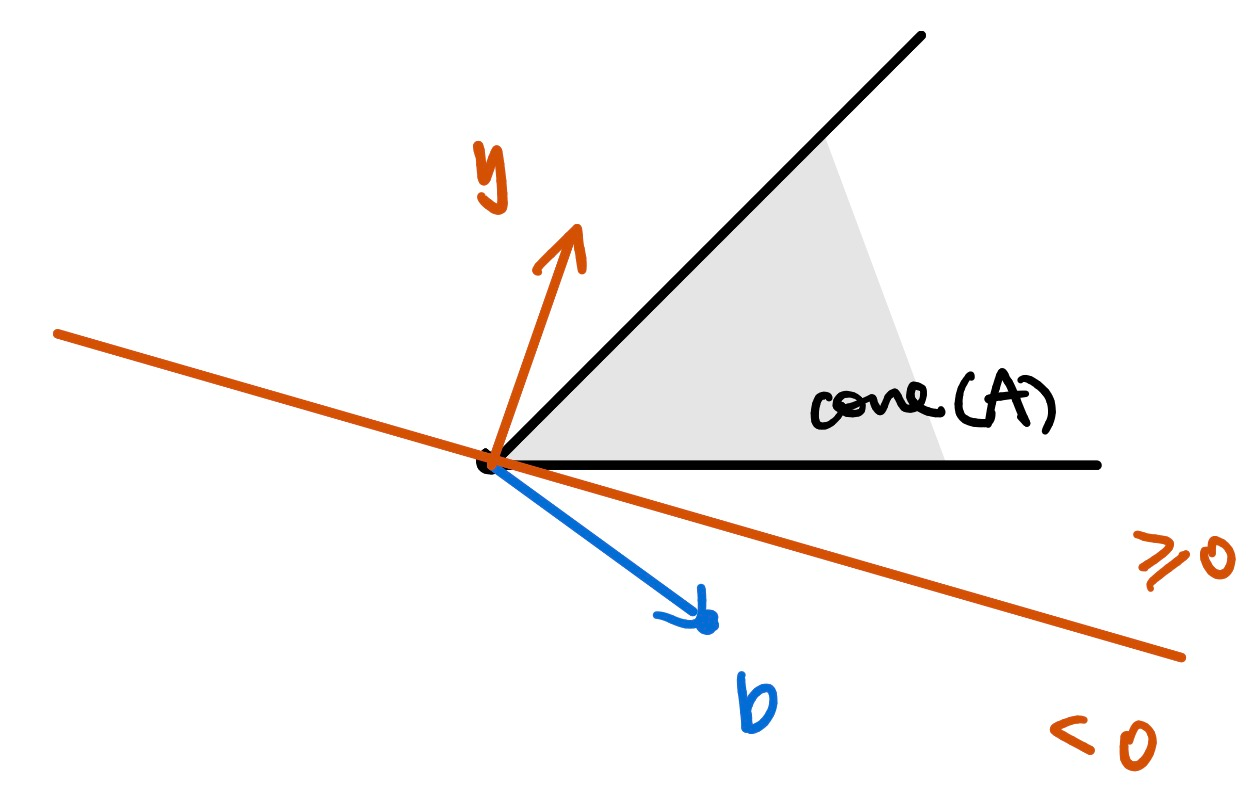
\includegraphics[width=0.45\linewidth]{figures/20261009201801658.png}
\end{center}

因此, $\bm{y}^\top \bm{A} \geq \bm{0}^\top$ , $\bm{y}^\top \bm{b} < 0$ 就是原问题不可行性的一个 certificate. 如果这个成立, 就一定不可行; 反之亦然.

需要说明的是, 该视角的严格证明需要依赖于 \emph{$\text{cone}(\bm{A})$ 是闭凸集} 这一事实, 而其 closedness 的证明并不是 trivial 的, 需要依赖于 Carathéodory 定理. 不过这里不妨承认之.


% Source Markdown lines 901–909
\begin{exampleblock}[{Farkas lemma in No-arbitrage financial market}]
考虑一个单期金融市场.

\begin{itemize}
\item {}市场有 $n$ 种资产, 在期末有 $m$ 种可能的状态. 记 payoff matrix 为 $\bm{R} \in \mathbb{R}^{m \times n}$, 其中 $\bm{R}_{ij}$ 表示第 $j$ 种资产在第 $i$ 种期末市场状态下的收益.


\item {}记 $\bm{x} \in \mathbb{R}^n$ 为投资组合的权重且允许为负 (short selling). 则投资组合在期末的收益为 $\bm{w} = \bm{R}\bm{x} \in \mathbb{R}^m$.


\item {}另外当前的投资组合价格为 $\bm{p} \in \mathbb{R}^n$, 故持有该投资组合的成本为 $\bm{p}^\top \bm{x}$.


\end{itemize}

在金融市场中, 一个投资组合 $\bm{x}$ 在此处所讨论的严格负初始成本意义下是可套利的, 当存在某种组合 $\bm{x}$ 使得 $\bm{R}\bm{x} \geq \bm{0}$ 且 $\bm{p}^\top \bm{x} < 0$. 也即, 在期末的收益是非负的, 且在期初的成本是负的 (即不需要投入资金).

故为使得市场无套利, 则必须不存在这样的 $\bm{x}$. 根据 Farkas lemma, 则等价于存在 $\bm{q}\in \mathbb{R}^m_{\geq 0}$ 使得 $\bm{R}^\top \bm{q} = \bm{p}$, 或等价地对于每个资产 $j=1,\dots,n$，有 $\bm{p}_j = \sum_{i=1}^m \bm{R}_{ij} \bm{q}_i$. 也即, 存在一个非负的状态价格向量 $\bm{q}$, 使得每个资产的价格等于其在各个状态下的收益的加权和 (权重为 $\bm{q}$). 若 $\sum_i q_i > 0$, 归一化后可看成概率分布下的期望收益再乘以 $\sum_i q_i$. 这就是金融市场中无套利定价的基本原理.

\end{exampleblock}

\subsection{Variants of Farkas lemma and General Discussion of Alternative System}

\emph{\textbf{Some Classic Variants}}


% Source Markdown lines 915–918
\begin{propositionblock}[{Some Classic Variants}]
如下是 Farkas lemma 的一些常见变体, 其都是择一成立的, 有时也称之为 alternative system.

\begin{itemize}
\item {}Gordan lemma: $\bm{A}\bm{x} < 0$ $\text{与}$ $\bm{A}^\top \bm{y} = 0,~ \bm{y} \geq 0,~ \bm{y} \neq 0$.


\item {}$\bm{A}\bm{x} \leq 0$, $\bm{x} \geq 0$, $\bm{c}^\top \bm{x} > 0$ $\text{与}$ $\bm{A}^\top \bm{y} \geq \bm{c}$, $\bm{y} \geq 0$.


\item {}$\bm{A}\bm{x} \leq \bm{0}$, $\bm{B}\bm{x} = \bm{0}$, $\bm{c}^\top \bm{x} > 0$ $\text{与}$ $\bm{A}^\top \bm{y} + \bm{B}^\top \bm{z} = \bm{c}$, $\bm{y} \geq 0$, $\bm{z}$ 任意.


\end{itemize}

\end{propositionblock}

\emph{\textbf{Alternative system}}

隐约感觉, Farkas lemma 并不是一个特殊的定理, 其背后有着一套更为普遍的分析框架. 故我们尝试讨论其背后的更一般的行为.

考虑一个集合 $\mathcal{S} \subseteq \mathbb{R}^n$，且给定 $\bm{b} \in \mathbb{R}^n$，可行性问题即为判断 $\bm{b} \in \mathcal{S}$ 是否成立, 这是一个 membership problem. 其一般有两种方法来判断 $\bm{b} \in \mathcal{S}$ 是否成立:

\begin{itemize}
\item {}Constructive: 如果我们认为 $\bm{b} \in \mathcal{S}$，则可以直接给出 $\bm{b}$ 属于 $\mathcal{S}$ 的构造，并证明其确实符合 $\mathcal{S}$ 的定义.


\item {}Certificate: 如果我们认为 $\bm{b} \notin \mathcal{S}$，则可以找到某些易于检查的性质 (certificate), 使得: 所有 $\mathcal{S}$ 中的元素定满足这些性质, 而 $\bm{b}$ 不满足这些性质.

\begin{quote}
注意, 从逻辑上, 我们总可以说 $P \lor \neg P$，而 alternative system 之所以有意义, 是因为其给一个抽象的否命题提供了一组具体的条件, 甚至是一组线性泛函的条件, 这使得我们可以非常容易地检查条件的成立与否.

\end{quote}


\end{itemize}

而对于一个非空闭凸集 $\mathcal{S}$，separation theorem 给出了一个非常自然的 certificate.

\begin{itemize}
\item {}其自然地将一个集合的属于性问题, 转化为了一个线性不等式的成立性问题.

\begin{itemize}
\item {}按照几何的视角, 条件 $\bm{x} \geq 0, \bm{A}\bm{x}$ 就定义了一个凸锥 $\mathcal{S}:= \text{cone}(\bm{A})$，而不存在 $\bm{x} \geq 0$ 使得 $\bm{A}\bm{x} = \bm{b}$，则说明 $\bm{b} \notin \mathcal{S}$, 即存在锥外点 $\bm{b}$. 则根据 separation theorem, 存在一个超平面将 $\bm{b}$ 和 $\mathcal{S}$ 分开, 其法向量为 $\bm{y}$.


\item {}而超平面又可以通过 support function 来刻画, $\bm{b} \notin \mathcal{S}$ $\iff$ 存在 $\bm{y}$ 使得 $\bm{y}^\top \bm{b} > \sigma_{\mathcal{S}}(\bm{y}) = \sup_{\bm{x} \in \mathcal{S}} \bm{y}^\top \bm{x}$.


\end{itemize}


\item {}因此, 更本质地从分析的角度, 其是将集合的属于性问题, 通过一个线性泛函给出了一个易于检查的条件 (这是线性的). 欲判断 $\bm{b} \in \mathcal{S}$ 是否成立, 只需要检查 $\bm{b}$ 通过一个线性泛函得到的评分, 是否大于所有 $\mathcal{S}$ 中的元素通过这个线性泛函得到的评分即可. 而在有限维的欧式空间中, 每一个线性泛函都可以表示成与某个向量的内积, 这也就引入了向量 $\bm{y}$.


\end{itemize}

继续更深入考虑 $\bm{y}$. 通过下面的思考角度, 我们或许也可以任意构造给定线性系统 feasibility 的 certificate.

\begin{itemize}
\item {}先考虑一个简单的线性系统:

\[
\begin{aligned}
  x_1 + x_2 &\leq 1,\\
  -x_1 - x_2 &\leq -3.
\end{aligned}
\]

显然这个系统无解, 因为两式相加即有 $0 \leq -2$, 矛盾.


\item {}故进一步考虑 $\bm{A}_i^\top \bm{x} \leq b_i,~ i=1,\dots,m$，仿照前面的过程, 若能找到一些 $\bm{y}_i \geq 0$，使得 $\sum_{i=1}^m \bm{A}_i \bm{y}_i = 0$，则可以类似地对每个 $\bm{A}_i^\top \bm{x} \leq b_i$ 乘以 $\bm{y}_i$，然后相加, 得到

\[
\sum_{i=1}^m \bm{A}_i^\top \bm{x} \bm{y}_i = 0 \leq \sum_{i=1}^m b_i \bm{y}_i.
\]

由于 $\bm{y}_i \geq 0$ , 其不改变不等式的方向. 若进一步又要求 $\sum_{i=1}^m b_i \bm{y}_i < 0$，就可以构造矛盾, 从而说明原系统无解.


\item {}而且从上述的讨论还可以看到, 如果原始的约束是不等式约束 $\bm{A}_i^\top \bm{x} \leq b_i$，则对应的 certificate 是 $\bm{y}_i \geq 0$ 也需要通过不等式约束来保证符号不变; 反之若是等式 $\bm{A}_i^\top \bm{x} = b_i$，则对应的 certificate 是 $\bm{y}_i$ 可以是任意实数. 这在上述最后一个变体 $\bm{A}^\top \bm{y} + \bm{B}^\top \bm{z} = \bm{c}$ 中就体现了出来, 其中 $\bm{y}$ 对应不等式约束, $\bm{z}$ 对应等式约束.


\end{itemize}

\subsection{Tricks of proving Farkas lemma}

若在偏应试的角度证明 Farkas lemma, 则可以考虑通过标准化的方法统一证明. 为作区分, 这里记最终的 alternative system 为

\[
\begin{aligned}
  \bm{M}\bm{w} & = \bm{h},\quad &&\bm{w} \geq 0,\quad \text{(System 1)}\\
  \bm{M}^\top \bm{z} &\geq 0,\quad &&\bm{h}^\top \bm{z} < 0. \quad \text{(System 2)}
\end{aligned}
\]

其中 $\bm{z}$ 是自由变量. 故此时的问题重点在于将给定的线性系统转为此标准型.


% Source Markdown lines 967–973
\begin{exampleblock}{}
如下线性系统有且仅有一个 alternative system 成立:

\[
\begin{aligned}
  \bm{A}\bm{x} &\leq \bm{0},\quad &&\bm{x} \geq 0,\quad \bm{b}^\top \bm{x} > 0, \quad \text{(System 1)}\\
  \bm{A}^\top \bm{y} &\geq \bm{b},\quad &&\bm{y} \geq 0. \quad \quad \text{(System 2)}
\end{aligned}
\]

\end{exampleblock}


% Source Markdown lines 975–997
\begin{proof}{}
首先处理 System 1.

\begin{itemize}
\item {}为进行标准化, 首先要处理 $\bm{b}^\top \bm{x} > 0$ 这个 strict inequality.

\begin{itemize}
\item {}注意到有如下等价关系: $\bm{A}\bm{x} \leq \bm{0}$, $\bm{x} \geq 0$, $\bm{b}^\top \bm{x} > 0$ $\iff$ $\bm{A}\bm{x} \leq \bm{0}$, $\bm{x} \geq 0$, $\bm{b}^\top \bm{x} = 1$. 也即, 由于前两项是 homogeneous 的, 故可以通过缩放 $\bm{x}$ 将 $\bm{b}^\top \bm{x} > 0$ 归一化为 $\bm{b}^\top \bm{x} = 1$.


\item {}这是因为, 若 $\bm{A}\bm{x} \leq \bm{0}$, $\bm{x} \geq 0$ 成立, 则对于任意 $\alpha > 0$，有 $\bm{A}(\alpha \bm{x}) = \alpha \bm{A}\bm{x} \leq \bm{0}$, $\alpha \bm{x} \geq 0$, 故取 $\bm{\hat{x}} = \frac{\bm{x}}{\bm{b}^\top \bm{x}}$ 即可得到 $\bm{b}^\top \bm{\hat{x}} = 1$.


\end{itemize}


\item {}接着, 对于 $\bm{A}\bm{x} \leq \bm{0}$, 可以引入 slack variable $\bm{s} \geq 0$，将其转化为等式约束 $\bm{A}\bm{x} + \bm{s} = \bm{0}$.


\item {}最终, 将 $\bm{x}$ 和 $\bm{s}$ 组合为 $\bm{w} = [\bm{x}; \bm{s}]$，则原问题可以转化为标准形式:

\[
\bm{M}\bm{w} = \begin{bmatrix} \bm{A} & \bm{I}_m \\ \bm{b}^\top & 0 \end{bmatrix} \begin{bmatrix} \bm{x} \\ \bm{s} \end{bmatrix} = \begin{bmatrix} \bm{0}_m \\ 1 \end{bmatrix} = \bm{h},\quad \bm{w} \geq 0.
\]


\end{itemize}

故根据 Farkas lemma, System 1 有解当且仅当 System 2: $\bm{M}^\top \bm{z} \geq 0$, $\bm{h}^\top \bm{z} < 0$ 无解. 故下要证明 System 2 无解与题设 $\bm{A}^\top \bm{y} \geq \bm{b}$, $\bm{y} \geq 0$ 无解等价.

\begin{itemize}
\item {}不妨将 $\bm{z} = \begin{bmatrix} \bm{z}_1 \\ z_2 \end{bmatrix}$，其中 $\bm{z}_1 \in \mathbb{R}^m$, $z_2 \in \mathbb{R}$. 则 System 2 可以写为:

\[
\begin{aligned}
  \bm{A}^\top \bm{z}_1 + z_2 \bm{b} &\geq 0, \quad \bm{z}_1 \geq 0,\quad z_2 < 0.
\end{aligned}
\]


\item {}再次根据齐次性, 任意满足条件的 $(\bm{z}_1, z_2)$, 都可以引入 $\beta > 0$, 使得 $\bm{A}^\top (\beta \bm{z}_1) + (\beta z_2) \bm{b} \geq 0$, $\beta \bm{z}_1 \geq 0$, $\beta z_2 < 0$. 故不妨令 $\beta = -\frac{1}{z_2} > 0$，则有 $\bm{A}^\top (-\frac{\bm{z}_1}{z_2}) - \bm{b} \geq 0$, $-\frac{\bm{z}_1}{z_2} \geq 0$, $-\frac{1}{z_2} z_2 = -1 < 0$. 故令 $\bm{y} = -\frac{\bm{z}_1}{z_2} \geq 0$，则 System 2 无解等价于 $\bm{A}^\top \bm{y} \geq \bm{b}$, $\bm{y} \geq 0$ 无解.


\end{itemize}

\end{proof}

\section{The geometry of LP}

本小节主要参考 [Bertsimas, § 2 和 § 4.8, 4.9].

\subsection{Extreme points, vertices, and basic feasible solutions}

\subsubsection{Extreme points, vertices and basic feasible solutions}

在初等的 LP 学习过程中, 往往会有 LP 的解在角落处取得最优值的结论. Bertsimas 的书中从三个角度论述了 '角落' 这个概念, 并且给出了它们之间的等价性.


% Source Markdown lines 1009–1022
\begin{defblock}[{Extreme points, vertices and basic feasible solutions}]
\begin{itemize}
\item {}\textbf{Extreme Point.} 如果一个点 $\bm{x} \in \mathcal{P}$ 不能表示为 $\mathcal{P}$ 中两个不同点的非平凡凸组合, 则称 $\bm{x}$ 是 $\mathcal{P}$ 的 extreme point.

\begin{center}
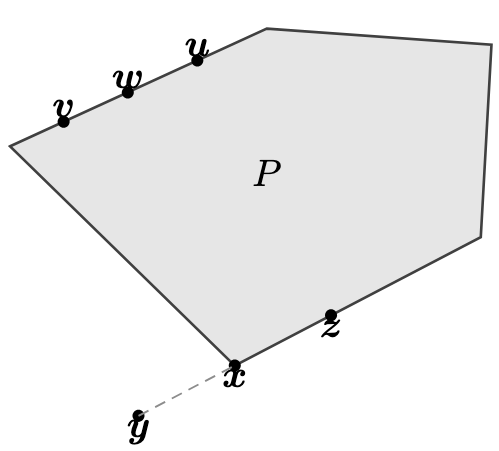
\includegraphics[width=0.3\linewidth]{figures/20261023141151.png}
\end{center}

\begin{itemize}
\item {}三角形的三个顶点都是 extreme points, 圆盘边界上的所有点都是 extreme points, 半空间没有 extreme points.


\end{itemize}


\item {}\textbf{Vertex.} 对于 Polyhedron $\mathcal{P}$，定义 $\bm{x} \in \mathcal{P}$ 是 $\mathcal{P}$ 的 vertex, 如果存在 $\bm{c} \in \mathbb{R}^n$ 使得对任意 $\bm{y} \in \mathcal{P} \setminus \{\bm{x}\}$，有 $\bm{c}^\top \bm{x} < \bm{c}^\top \bm{y}$.

\begin{center}
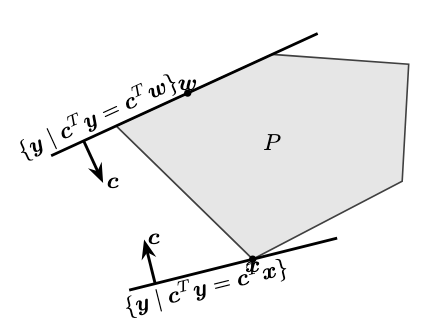
\includegraphics[width=0.3\linewidth]{figures/20261023141406.png}
\end{center}

\begin{itemize}
\item {}Vertex 可以理解为: 若 supporting hyperplane 与 $\mathcal{P}$ 唯一相交于 $\bm{x}$，则 $\bm{x}$ 是 vertex.


\end{itemize}


\item {}\textbf{Basic feasible solution.} 考虑由线性等式和不等式构成的 polyhedron $\mathcal{P} \subseteq \mathbb{R}^n$，且 $\bm{x} \in \mathbb{R}^n$. 称 $\bm{x}$ 是 basic solution, 如果其所有等式约束都是 active 的, 且在所有 active constraints 中 (可能是等式或不等式约束) 恰有 $n$ 个约束是线性无关的. 若进一步 $\bm{x}$ 是 feasible 的, 则称 $\bm{x}$ 是 basic feasible solution (BFS).

\begin{itemize}
\item {}\textbf{Active constraints.} 分别记 LP 中的三种约束为 $\mathcal{M}_1 := \{i: \bm{a}_i^\top \bm{x} \geq b_i\}$, $\mathcal{M}_2 := \{i: \bm{a}_i^\top \bm{x} \leq b_i\}$, $\mathcal{M}_3 := \{i: \bm{a}_i^\top \bm{x} = b_i\}$. 若对于 $\bm{x}^* \in \mathcal{P}$，有 $\bm{a}_i^\top \bm{x}^* = b_i$，则称约束 $i$ 是 active 的.


\end{itemize}


\end{itemize}

\end{defblock}


% Source Markdown lines 1024–1027
\begin{lemmablock}{}
首先根据线性代数给出如下命题作为引理. 给定 $\bm{x}^* \in \mathbb{R}^n$, 令 $\mathcal{I} = \{i: \bm{a}_i^\top \bm{x}^* = b_i\}$. 则如下命题等价:

\begin{enumerate}
\item {}线性系统 $\bm{a}_i^\top \bm{x} = b_i,~ i \in \mathcal{I}$ 有唯一解 $\bm{x}^*$.


\item {}存在 $n$ 个线性无关的约束 $\bm{a}_{i_1}, \dots, \bm{a}_{i_n}$, 其中 $i_j \in \mathcal{I}$.


\item {}所有 $\bm{a}_i,~ i \in \mathcal{I}$ 张成的空间是 $\mathbb{R}^n$.


\end{enumerate}

\end{lemmablock}


% Source Markdown lines 1029–1032
\begin{propositionblock}{}
据此立即得到, 由上述三个角度定义的 extreme point, vertex 和 basic feasible solution 三者是等价的: 对于 $\mathcal{P}$ 是非空的 polyhedron, 且 $\bm{x}^* \in \mathcal{P}$, 有

\begin{enumerate}
\item {}$\bm{x}^*$ 是 $\mathcal{P}$ 的 extreme point.


\item {}$\bm{x}^*$ 是 $\mathcal{P}$ 的 vertex.


\item {}$\bm{x}^*$ 是 $\mathcal{P}$ 的 basic feasible solution.


\end{enumerate}

\end{propositionblock}

因此对应如下 extreme point 的判定定理.


% Source Markdown lines 1036–1036
\begin{thmblock}[{Extreme point characterization}]
给定 Polyhedron $\mathcal{P} \subseteq \mathbb{R}^n$，则 $\bm{x}^* \in \mathcal{P}$ 是 $\mathcal{P}$ 的 extreme point 当且仅当 $\bm{x}^*$ 的 active constraints 中有 $n$ 个线性无关的约束.

\end{thmblock}

\begin{quote}
Note.
注意, 上述的讨论与具体的 $\mathcal{P}$ 的表示是无关的.

\end{quote}

\subsection{Polyhedral in Standard Form}

\subsubsection{Basic solution characterization in standard form}

下面考虑 polyhedron 的标准形式, 并将上述讨论在标准形式下进行具体化. 具体而言, 给定 $\mathcal{P} = \{\bm{x} \in \mathbb{R}^n: \bm{A}\bm{x} = \bm{b},~ \bm{x} \geq 0\}$，其中 $\bm{A} \in \mathbb{R}^{m \times n}$ 且 $\text{rank}(\bm{A}) = m < n$ (行满秩). 即, 共有 $n$ 个变量, $m$ 个线性等式约束.
这里记 $\bm{A} = [\bm{A}_1, \dots, \bm{A}_n]$，其中 $\bm{A}_i \in \mathbb{R}^m$ 是 $\bm{A}$ 的第 $i$ 列.

给定 $\bm{x}^* \in \mathcal{P}$, 我们想讨论其是否是 extreme point / vertex / basic solution.

\begin{itemize}
\item {}注意到, 由于 $\bm{A}\bm{x}^* = \bm{b}$, 首先这些等式约束就天然地提供了 $m$ 个 active constraints. 进一步, 由于假设 $\bm{A}$ 是行满秩的, 故这 $m$ 个 active constraints 是线性无关的.


\item {}根据上述的极点判定定理, 若 $\bm{x}^*$ 是 BS, 则需要总共 $n$ 个 linear independent active constraints. 故还需要额外的 $n-m$ 个 active constraints. 因此我们要选择 $(n-m)$ 个不等式约束 $\bm{x} \geq 0$ 使其为 active constraints. 也即, 需要选择 $(n-m)$ 个 $\bm{x}^*_i = 0$.

\begin{itemize}
\item {}从几何的角度理解, 对于一个 $\mathbb{R}^n$ 的空间, 等式 $\bm{A}\bm{x} = \bm{b}$ (在行满秩条件下) 确定了 $m$ 个维度, 留下了 $(n-m)$ 个自由度. 也即, $\bm{A} \bm{x} = \bm{b}$ 的解集 (即 $m$ 个超平面的交集) 是一个 $(n-m)$ 维的 affine space. 因此, 若想唯一确定一个点, 则要消除余下的 $(n-m)$ 个自由度, 也即需要 $(n-m)$ 个不等式约束 $\bm{x} \geq 0$ 使其为 active constraints.


\item {}如下图所示, 这是一个 $n=6$, $m=4$ 的例子. 也即, 在一个 $\mathbb{R}^6$ 的空间中, 通过 $\bm{A}\bm{x} = \bm{b}$ 的 $4$ 个等式约束, 确定了一个 $2$ 维的 affine space (即图中所展示的空间). 此外, 还有 $6$ 个不等式约束 $\bm{x} \geq 0$, 即为图中的 $6$ 条直线. 任选两条直线的交点, 即为令这两个约束为 active constraints, 则可以唯一确定一个点. 也即, 该点是 basic solution. 不过 Basic solution 并不一定是 feasible 的.


\end{itemize}

\begin{center}
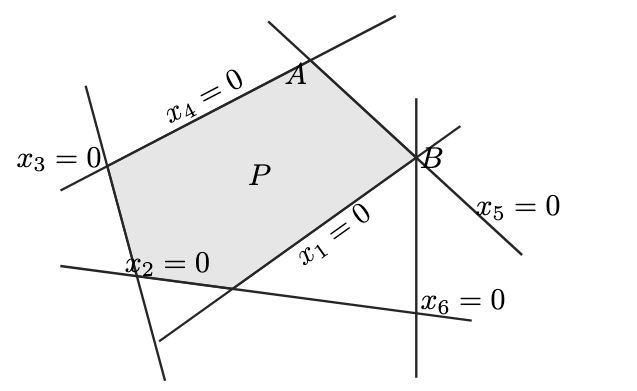
\includegraphics[width=0.5\linewidth]{figures/20261023150428.png}
\end{center}


\item {}我们已经说明, 要选择 $(n-m)$ 个 $\bm{x}^*_i = 0$ 来作为 active constraints. 这样的选择并不唯一, 但也不是任意的. 这是因为, 如果新增的约束与原有的 $m$ 个等式约束线性相关, 则这样的选择是无效的.


\end{itemize}

故, 可以将上述的讨论总结为如下定理.


% Source Markdown lines 1062–1064
\begin{thmblock}[{Basic Solution Characterization in Standard Form}]
考虑标准形式. $\bm{x}^* \in \mathbb{R}^n$ 是 $\mathcal{P}$ 的 basic solution 当且仅当: 所有等式约束 $\bm{A}\bm{x} = \bm{b}$ 都是 active 的; 且存在 $m$ 个 indices $B(1), \dots, B(m)$ 使得 (1) $\bm{A}$ 的对应列向量 $\bm{A}_{B(1)}, \dots, \bm{A}_{B(m)}$ 是线性无关的, 且 (2) 对于任意 $j \notin \{B(1), \dots, B(m)\}$，有 $\bm{x}^*_j = 0$.

\begin{itemize}
\item {}注意, 这里仅要求 $\bm{x}^*$ 是 basic solution, 并不要求其是 feasible 的. 若进一步要求 $\bm{x}^* \geq 0$，则称其为 basic feasible solution (BFS).


\end{itemize}

\end{thmblock}


% Source Markdown lines 1066–1066
\begin{defblock}[{Basic and non-basic variables}]
为方便叙述, 称 $\bm{A}_{B(1)}, \dots, \bm{A}_{B(m)}$ 为 basic columns, 对应的变量 $\bm{x}_{B(1)}, \dots, \bm{x}_{B(m)}$ 为 basic variables, 其余的变量为 non-basic variables. 并且 wlog 可以将 $\bm{A}$ 进行列重排, 使得 $\bm{A} = [\bm{B}, \bm{N}]$，其中 $\bm{B} = [\bm{A}_{B(1)}, \dots, \bm{A}_{B(m)}] \in \mathbb{R}^{m \times m}$ 是 basic matrix, $\bm{N} = [\bm{A}_{j_1}, \dots, \bm{A}_{j_{n-m}}] \in \mathbb{R}^{m \times (n-m)}$ 是 non-basic matrix. 对应的变量为 $\bm{x} = [\bm{x}_B; \bm{x}_N]$.

\end{defblock}

\subsubsection{Constructing basic solution}

利用上述定理, 给出如下构造 BS 的方法. 给定 $\mathcal{P} = \{\bm{x} \in \mathbb{R}^n: \bm{A}\bm{x} = \bm{b},~ \bm{x} \geq 0\}$:

\begin{enumerate}
\item {}选择 $m$ 个线性无关的列向量 $\bm{A}_{B(1)}, \dots, \bm{A}_{B(m)}$，并将其作为 basic columns. 其余的列向量为 non-basic columns. 并且按照上述的约定, 将 $\bm{A}$ 进行列重排, 得到 $\bm{A} = [\bm{B}, \bm{N}]$, 对应的变量为 $\bm{x} = [\bm{x}_B; \bm{x}_N]$.


\item {}将 non-basic variables 置为 $0$, 即 $\bm{x}_N = 0$.


\item {}由 $\bm{A}\bm{x} = \bm{b}$ 可得 $\bm{B}\bm{x}_B = \bm{b}$, 由于 $\bm{B}$ 是非奇异的, 故可解得 $\bm{x}_B = \bm{B}^{-1}\bm{b}$.


\end{enumerate}

最终, 得到 $\bm{x} = [\bm{x}_B; \bm{x}_N]$ 即为一个 basic solution. 若进一步 $\bm{x} \geq 0$，则为 basic feasible solution.


% Source Markdown lines 1079–1112
\begin{exampleblock}{}
考虑 $\bm{A} \bm{x} = \bm{b}$ 为

\[
\begin{pmatrix}
  1 & 1 & 2 & 1 & 0 & 0 & 0\\
  0 & 1 & 6 & 0 & 1 & 0 & 0\\
  1 & 0 & 0 & 0 & 0 & 1 & 0\\
  0 & 1 & 0 & 0 & 0 & 0 & 1
\end{pmatrix}
\begin{pmatrix}
  x_1\\x_2\\x_3\\x_4\\x_5\\x_6\\x_7
\end{pmatrix}
=
\begin{pmatrix}
  8 \\ 12 \\ 4 \\ 6
\end{pmatrix}.
\]

则 $\bm{A}$ 的 rank 为 $4$, 对应的 basic solution 需要选择 $4$ 个线性无关的列向量作为 basic columns. 例如, 选择 $\bm{A}_4, \bm{A}_5, \bm{A}_6, \bm{A}_7$ 作为 basic columns, 则 non-basic columns 为 $\bm{A}_1, \bm{A}_2, \bm{A}_3$. 因此得到

\[
\bm{B} =
\begin{pmatrix}
  1 & 0 & 0 & 0\\
  0 & 1 & 0 & 0\\
  0 & 0 & 1 & 0\\
  0 & 0 & 0 & 1
\end{pmatrix},\quad
\bm{N} =
\begin{pmatrix}
  1 & 1 & 2\\
  0 & 1 & 6\\
  1 & 0 & 0\\
  0 & 1 & 0
\end{pmatrix}.
\]

将 non-basic variables 置为 $0$, 即 $\bm{x}_N = \bm{0}$. 对应 $\bm{x}_B = \bm{B}^{-1}\bm{b} = (8, 12, 4, 6)^\top$. 故最终得到 basic solution 为 $\bm{x} = (0, 0, 0, 8, 12, 4, 6)^\top$. 由于 $\bm{x} \geq 0$, 故其为 basic feasible solution.

\end{exampleblock}

\subsubsection{Column space perspective of basic solution}

进一步通过列空间的角度来理解 basic solution 的构造. 考虑 $m=2$, $n=4$ 的例子, 如下图所示. 因此 $\bm{A}\bm{x} = \bm{A}_1 x_1 + \bm{A}_2 x_2 + \bm{A}_3 x_3 + \bm{A}_4 x_4 = \bm{b}$, 可以看作是通过四种不同的资源 $\bm{A}_1, \bm{A}_2, \bm{A}_3, \bm{A}_4$ 的线性组合来得到 $\bm{b}$. 由于 $\text{rank}(\bm{A}) = 2$, 故 $\bm{b}$ 可以由任意两个线性无关的列向量的线性组合来表示.

\begin{itemize}
\item {}$\bm{A}_1, \bm{A}_2$ 是线性无关的, 故 $\bm{b}$ 可以由 $\bm{A}_1, \bm{A}_2$ 的线性组合来表示, 故可以构成一个 basis. 然而, 为了表示 $\bm{b}$, $x$ 的系数需要为负数, 故其不是 basic feasible solution.


\item {}$\bm{A}_1, \bm{A}_3$ 是线性无关的, 故 $\bm{b}$ 可以由 $\bm{A}_1, \bm{A}_3$ 的线性组合来表示, 且系数均为非负数, 故其是 basic feasible solution.


\item {}$\bm{A}_1, \bm{A}_4$ 是线性相关的, 故不能构成 basis, 也即不能表示 $\bm{b}$.


\end{itemize}

\begin{center}
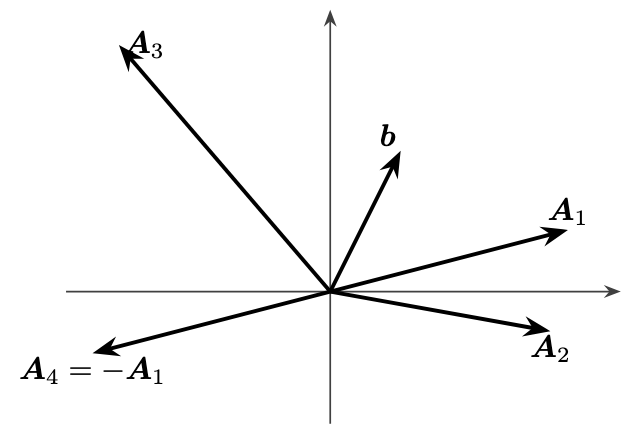
\includegraphics[width=0.5\linewidth]{figures/20261023153354.png}
\end{center}

\subsubsection{Full row rank assumption}

最后说明, 上述对于 $\bm{A}$ 的行满秩假设是 wlog 的. 只要 $\mathcal{P}$ 是非空的 polyhedron, 则即使 $\bm{A}$ 不是行满秩的, 也可以直接丢弃冗余的行约束, 使得余下的约束是行满秩的, 而不改变 basic solution 的构造.

例如考虑约束:

\[
\begin{aligned}
  2x_1 + x_2 + x_3 &= 2,\\
  x_1 + x_2 &= 1,\\
  x_1 + x_3 &= 1,\\
  x_1, x_2, x_3 &\geq 0.
\end{aligned}
\]

不难发现, 第一个约束是冗余的, 因为其可以由后两个约束线性组合得到. 丢弃第一个约束, 则剩下的约束是行满秩的, 且不改变 basic solution 的构造.

\subsection{Degeneracy}

\subsubsection{Basis and basic solution}

考虑 basis matrix 和 basic solution 的关系, 可以发现: 一个 basis 只能对应一个 basic solution, 但一个 basic solution 可能对应多个 basis.

\begin{itemize}
\item {}对于标准形式 $\mathcal{P}$, 通过上述的构造方法, 选择 $m$ 个线性无关的列向量作为 basic columns 构造 $\bm{B}$, 令其余 $n-m$ 个对应的 $\bm{x}_N = 0$, 则可以求解 $\bm{x}_B = \bm{B}^{-1}\bm{b}$ 得到 basic solution $\bm{x} = [\bm{x}_B; \bm{x}_N]$. 由于 $\bm{B}$ 是非奇异的, 故 $\bm{x}_B$ 是唯一的.


\item {}然而反过来, 可能存在多个不同的 basis 对应同一个 basic solution. 这是因为, 在求解 $\bm{x}_B = \bm{B}^{-1}\bm{b}$ 时, 可能存在某些 $\bm{x}_B$ 的分量为 $0$. 而这些分量为 $0$ 的 basic variables, 也可以被视为 non-basic variables, 从而可以选择不同的 basic columns 来构造不同的 basis. 这就是 degeneracy 的来源.


\end{itemize}

例如考虑 $\mathbb{R}^3$ 空间中的如下两个约束:

\[
\begin{cases}
  x_1 + x_3 &= 1,\\
  x_2 + x_3 &= 0.
\end{cases}
\]

则对应的 $\bm{A}_1 = (1, 0)^\top$, $\bm{A}_2 = (0, 1)^\top$, $\bm{A}_3 = (1, 1)^\top$, $\bm{b} = (1, 0)^\top$.

\begin{itemize}
\item {}若选择 $\bm{A}_1, \bm{A}_2$ 作为 basic columns, 则 $\bm{B}_1 = \begin{pmatrix} 1 & 0 \\ 0 & 1 \end{pmatrix}$, 则 $\bm{x}_B = \bm{B}_1^{-1} \bm{b} = (1, 0)^\top$, 对应的 basic solution 为 $\bm{x} = (1, 0, 0)^\top$.


\item {}若选择 $\bm{A}_1, \bm{A}_3$ 作为 basic columns, 则 $\bm{B}_2 = \begin{pmatrix} 1 & 1 \\ 0 & 1 \end{pmatrix}$, 则 $\bm{x}_B = \bm{B}_2^{-1} \bm{b} = (1, 0)^\top$, 对应的 basic solution 为 $\bm{x} = (1, 0, 0)^\top$.


\end{itemize}

\subsubsection{Degeneracy}


% Source Markdown lines 1164–1166
\begin{defblock}[{Degeneracy}]
回顾, 点 $\bm{x}^* \in \mathbb{R}^n$ 是 basic solution, 当且仅当其满足所有的等式约束, 且在这个点处存在 $n$ 个线性无关的 active constraints.

此时, \textbf{若实际 active 的约束数大于 $n$, 则称 $\bm{x}^*$ 是 degenerate basic solution.} 因为在 $\mathbb{R}^n$ 空间中, 最多只有 $n$ 个线性无关的约束, 因此当活跃的约束数大于 $n$ 时, 必然存在冗余的约束, 也即存在某些约束是线性相关的. 这就导致了 degeneracy 的出现.

\end{defblock}


% Source Markdown lines 1168–1171
\begin{propositionblock}[{Degeneracy}]
故可以总结如下:

\begin{enumerate}
\item {}在一般形式下, basic solution $\bm{x} \in \mathbb{R}^n$ 是 degenerate 的, 当且仅当其对应的 active constraints 的数量大于 $n$.


\item {}在标准形式下, 一个 basic solution $\bm{x}^*$ 是 degenerate 的, 当且仅当其对应的 basic variables 中有至少一个为 $0$. 也即, 若 $\bm{x}^*$ 中 $0$ 的分量数大于 $n-m$ (即非 basic variables 的数量).


\item {}退化可能导致多个不同的 basis 对应同一个 basic solution (但不必然).


\end{enumerate}

\end{propositionblock}

此外指出, 退化和 feasibility 没有必然联系.

如下图 $B$ 点所示, 在该点有 3 个 active constraints, 但其所在的空间是 $\mathbb{R}^2$, 因此是 degenerate basic solution.

\begin{center}
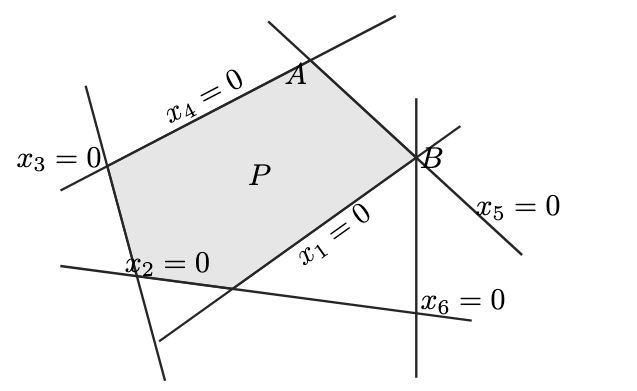
\includegraphics[width=0.5\linewidth]{figures/20261023150428.png}
\end{center}

如果 $\bm{A}, \bm{b}$ 是随机生成的, 则这种精确共线导致的 degeneracy 几乎不会发生. 但在实际问题中, 由于约束的特殊结构, 如一些现实的资源约束等, degeneracy 是很常见的.

此外, 退化并不是单纯由几何决定的. 同一个 polyhedron, 其不同的表示方式可能会导致不同的 degeneracy. 例如, 对于二维空间的第一象限 $\mathcal{P} := \{(x_1, x_2): x_1 \geq 0, x_2 \geq 0\}$, 若如此表示则原点 $(0, 0)$ 是非退化的 BFS; 但若将其表示为 $\mathcal{P} := \{(x_1, x_2): x_1 \geq 0, x_2 \geq 0, x_1 + x_2 \geq 0\}$, 则原点 $(0, 0)$ 是退化的 BFS.

\subsection{Existence of extreme points}

在之前的讨论中, 我们已知对于可行点 $\bm{x} \in \mathbb{R}^n$, $\bm{x}$ 是 extreme point 当且仅当其是 basic feasible solution, 当且仅当在 $\bm{x}$ 处有 $n$ 个线性无关的 active constraints (或 active constraints 的 normal vectors 张成 $\mathbb{R}^n$).

上述都是对于一个给定点 $\bm{x}$ 的讨论. 下面我们讨论, 对于一个给定的 polyhedron $\mathcal{P}$, 是否一定存在这样的 extreme point. 要意识到并不是所有的 polyhedron 都有 extreme points. 例如, 考虑半平面 $\mathcal{P} = \{(x_1, x_2): x_1 \geq 0\}$, 其包含一整条完整的直线, 是没有 extreme points 的.


% Source Markdown lines 1191–1194
\begin{thmblock}[{Existence of extreme points}]
给定 polyhedron $\mathcal{P} = \{\bm{x} \in \mathbb{R}^n: \bm{a}_i^\top \bm{x} \geq b_i,~ i=1,\dots,m\} \neq \varnothing$, 则如下三个条件等价:

\begin{enumerate}
\item {}$\mathcal{P}$ 有至少一个 extreme point.


\item {}$\mathcal{P}$ 不包含一条完整的直线. 其中, $\mathcal{P}$ 包含一条完整的直线, 当且仅当存在 $\bm{d} \neq \bm{0}$ 及 $\bm{x} \in \mathcal{P}$, 使得对于任意 $\lambda \in \mathbb{R}$, 有 $\bm{x} + \lambda \bm{d} \in \mathcal{P}$.


\item {}$\operatorname{span}\{\bm{a}_1, \dots, \bm{a}_m\} = \mathbb{R}^n$. (\emph{注意, 这里与判断某个点是 extreme point 的条件不同, 后者要求的是 active constraints 的 normal vectors 张成 $\mathbb{R}^n$, 而这里是所有约束的 normal vectors 张成 $\mathbb{R}^n$.})


\end{enumerate}

\end{thmblock}


% Source Markdown lines 1196–1221
\begin{proof}{}
\textbf{$(2) \implies (1)$}. 给定可行点 $\bm{x} \in \mathcal{P}$. 记 $\mathcal{I} = \{i: \bm{a}_i^\top \bm{x} = b_i\}$ 为 $\bm{x}$ 的 active constraints, $r = \text{dim}(\text{span}\{\bm{a}_i: i \in \mathcal{I}\})$.

\begin{itemize}
\item {}若 $r = n$, 则 $\bm{x}$ 是 extreme point, 命题成立.


\item {}若不然, $r<n$, 即 active 的约束的 normal vector 只能张成一个低于 $n$ 维的子空间. 此时在其正交补中一定存在非零向量 $\bm{d} \in \mathbb{R}^n$, 使得 $\bm{a}_i^\top \bm{d} = 0$ 对任意 $i \in \mathcal{I}$ 成立.

\begin{itemize}
\item {}因此, \textbf{沿着 $\bm{d}$ 的方向任意移动, 已有的 active constraints 依然 active}, 数学上即为, 对于 $\bm{y} = \bm{x} + \lambda \bm{d}$, 有 $\bm{a}_i^\top \bm{y} = \bm{a}_i^\top (\bm{x} + \lambda \bm{d}) = b_i$ 对任意 $i \in \mathcal{I}$ 成立.


\item {}对于非活跃约束 $j \notin \mathcal{I}$, 由于 $\bm{s}_j := \bm{a}_j^\top \bm{x} - b_j > 0$, 故沿着 $\bm{d}$ 的方向移动, 只要距离 $\lambda$ 足够小 (通过下式可以反推 $|\lambda| < \frac{\bm{s}_j}{2|\bm{a}_j^\top \bm{d}|}$, 对 $\bm{a}_j^\top \bm{d} \neq 0$; 若为零则无需限制), 就可以确保

\[
  \bm{a}_j^\top \bm{y} - b_j = \bm{a}_j^\top (\bm{x} + \lambda \bm{d}) - b_j = \bm{s}_j + \lambda \bm{a}_j^\top \bm{d} > 0.
\]

即, 沿着 $\bm{d}$ 的方向移动, 非活跃约束在小范围内依然保持非活跃.


\end{itemize}


\item {}根据 (2) 中题设, 由于 $\mathcal{P}$ 不包含一条完整的直线, 故沿着 $\bm{d}$ 或 $-\bm{d}$ 中至少一个方向移动一定会被阻挡, 即存在某位置 $\bm{x}' := \bm{x} + \lambda^\star \bm{d}$, 使得恰好某个非活跃 $k$ 约束变为活跃 (即 $\bm{a}_k^\top \bm{x}' = b_k$, $\bm{a}_k^\top \bm{x} > b_k$). 此时, $\bm{a}_k^\top \bm{x}' = \bm{a}_k^\top (\bm{x} + \lambda^\star \bm{d}) = b_k$, 故 $\lambda^\star \bm{a}_k^\top \bm{d} = b_k - \bm{a}_k^\top \bm{x} \neq 0$, 故 $\bm{a}_k^\top \bm{d} \neq 0$. 因此, $\bm{a}_k$ 与 $\bm{d}$ 不正交, 也即 $\bm{a}_k$ 不在 $\text{span}\{\bm{a}_i: i \in \mathcal{I}\}$ 中. 故 $\text{dim}(\text{span}\{\bm{a}_i: i \in \mathcal{I} \cup \{k\}\}) = r + 1$. 即只要不断沿着 $\bm{d}$ 的方向移动, 我们就终归会碰到新的约束点, 且此时会增加活跃约束的数量.


\item {}到达新的点 $\bm{x}'$ 后, 重新计算其 active constraints 的 normal vectors 张成的空间维度. 若仍然小于 $n$, 则继续沿着新的正交补方向移动, 直到活跃约束的 normal vectors 张成 $\mathbb{R}^n$. 由于 $\mathcal{P}$ 不包含完整直线, 故最终一定会到达一个 extreme point.


\end{itemize}

\textbf{$(3) \implies (2)$}. 反证法. 假设 $\mathcal{P}$ 包含一条完整的直线, 则存在 $\bm{d} \neq 0$ 及 $\bm{x} \in \mathcal{P}$, 使得对于任意 $\lambda \in \mathbb{R}$, 有 $\bm{x} + \lambda \bm{d} \in \mathcal{P}$.

\begin{itemize}
\item {}对于任意约束 $i = 1, \dots, m$, 由于直线上的任意点均在 $\mathcal{P}$ 中, 故有 $\bm{a}_i^\top (\bm{x} + \lambda \bm{d}) = \bm{a}_i^\top \bm{x}+ \lambda \bm{a}_i^\top \bm{d} \geq b_i$, 对任意 $\lambda \in \mathbb{R}$ 成立.


\item {}然而, 若 $\bm{a}_i^\top \bm{d} > 0$, 则当 $\lambda \to -\infty$ 时, $\bm{a}_i^\top (\bm{x} + \lambda \bm{d}) \to -\infty$, 与 $\bm{a}_i^\top (\bm{x} + \lambda \bm{d}) \geq b_i$ 矛盾. 反之若 $\bm{a}_i^\top \bm{d} < 0$, 则当 $\lambda \to +\infty$ 时, $\bm{a}_i^\top (\bm{x} + \lambda \bm{d}) \to -\infty$, 与 $\bm{a}_i^\top (\bm{x} + \lambda \bm{d}) \geq b_i$ 矛盾.


\item {}故只有 $\bm{a}_i^\top \bm{d} = 0$ 对于任意 $i = 1, \dots, m$ 成立. 也即, $\bm{d}$ 与所有约束的 normal vectors 正交. 然而由于 $\operatorname{span}\{\bm{a}_1, \dots, \bm{a}_m\} = \mathbb{R}^n$, 故 $\bm{d}$ 必须为 $0$, 与假设矛盾. 故 $\mathcal{P}$ 不包含完整直线.


\end{itemize}

\textbf{$(1) \implies (3)$}. 可以直接利用 extreme point 的判定定理. 若 $\bm{x}^*$ 是 extreme point, 则其为 BFS, 因此在 $\bm{x}^*$ 处有 $n$ 个线性无关的 active constraints, 故定有 $n$ 个线性无关的约束张成 $\mathbb{R}^n$.

\end{proof}


% Source Markdown lines 1223–1223
\begin{colblock}{}
因此立刻有推论: \emph{任何非空有界 polyhedron (故定不包含直线) 或任意非空标准型 polyhedron $\mathcal{P} = \{\bm{x} \in \mathbb{R}^n: \bm{A}\bm{x} = \bm{b},~ \bm{x} \geq 0\}$ (由于 $\mathcal{P} \subseteq \mathbb{R}^n_+$, 故不包含直线) 都至少有一个 extreme point, 即至少存在一个 basic feasible solution.} 这也为后续的 simplex 方法提供了理论基础.

\end{colblock}

\subsection{Optimality of extreme points}

下面正式进入一点线性规划的问题. 考虑如下问题:

\[
\min_{\bm{x} \in \mathcal{P}} \bm{c}^\top \bm{x} \tag{LP}
\]

其中 $\mathcal{P}$ 是某个 polyhedron.


% Source Markdown lines 1233–1234
\begin{thmblock}[{Optimality of extreme points}]
若 $\mathcal{P}$ 至少有一个 extreme point, 且该 LP 问题存在最优解 $\bm{x}^*$, 则至少有一个最优解是 extreme point.

\end{thmblock}


% Source Markdown lines 1236–1240
\begin{proof}{}
整体证明思路为: 首先找出原问题的全体最优解的集合, 并找出该最优解集内的 extreme point, 进而证明该 extreme point 也是原问题的极点.

\begin{itemize}
\item {}记 $\mathcal{Q} := \{\bm{x} \in \mathcal{P}: \bm{c}^\top \bm{x} = \min_{\bm{x} \in \mathcal{P}} \bm{c}^\top \bm{x}\}$ 为原问题的最优解集. 由于 $\mathcal{P}$ 是 polyhedron, 且 $\mathcal{Q}$ 是在 $\mathcal{P}$ 的基础上额外增加了一个线性约束 $\bm{c}^\top \bm{x} = \text{const}$, 故 $\mathcal{Q}$ 也是 polyhedron, 且题设的最优解存在性确保 $\mathcal{Q}$ 非空. 又因为 $\mathcal{P}$ 至少有一个 extreme point, 故定不包含直线, 故 $\mathcal{Q} \subseteq \mathcal{P}$ 也不包含直线. 根据极点存在性定理, $\mathcal{Q}$ 至少有一个 extreme point $\bm{x}^*$.


\item {}下用反证法证明 $\bm{x}^*$ 也是原问题的极点. 若不然, 则根据极点定义, 定存在不同的 $\bm{y}, \bm{z} \in \mathcal{P}$ 和 $\lambda \in (0, 1)$, 使得 $\bm{x}^* = \lambda \bm{y} + (1-\lambda) \bm{z}$. 由于 $\bm{y}, \bm{z} \in \mathcal{P}$, 且 $\bm{x}^*$ 是最优解, 故 $\bm{c}^\top \bm{y}  \geq \bm{c}^\top \bm{x}^* = \lambda \bm{c}^\top \bm{y} + (1-\lambda) \bm{c}^\top \bm{z}$, 且 $\bm{c}^\top \bm{z} \geq \bm{c}^\top \bm{x}^*$, 进而有 $\bm{c}^\top \bm{y} = \bm{c}^\top \bm{x}^* = \bm{c}^\top \bm{z}$, 故 $\bm{y}, \bm{z} \in \mathcal{Q}$. 这与 $\bm{x}^*$ 是 $\mathcal{Q}$ 的极点矛盾. 故 $\bm{x}^*$ 也是原问题的极点.


\end{itemize}

\end{proof}

该命题可以进一步加强如下.


% Source Markdown lines 1244–1244
\begin{thmblock}[{Optimality of extreme points}]
若 $\mathcal{P}$ 至少有一个 extreme point, 则 LP 问题 $\min_{\bm{x} \in \mathcal{P}} \bm{c}^\top \bm{x}$ 要么无下界, 要么存在最优解 $\bm{x}^*$在 extreme point 上.

\end{thmblock}


% Source Markdown lines 1246–1258
\begin{proof*}[{Proof}]
不妨记 $v:= \inf_{\bm{x} \in \mathcal{P}} \bm{c}^\top \bm{x}$, $\mathcal{P} := \{\bm{x} \in \mathbb{R}^n: \bm{A}\bm{x} \geq \bm{b}\}$. 由于 $\mathcal{P}$ 至少有一个 extreme point, 故定不包含完整直线. 对于某可行点 $\bm{x} \in \mathcal{P}$, 记 $\mathcal{I} = \{i: \bm{a}_i^\top \bm{x} = b_i\}$ 为 $\bm{x}$ 的 active constraints, $k = \text{dim}(\text{span}\{\bm{a}_i: i \in \mathcal{I}\})$ 即活跃约束的 normal vectors 张成的空间维度为该点的约束的 rank.

首先证明, 当目标函数有下界时, 对于任意可行点 $\bm{x} \in \mathcal{P}$, 都存在一个 BFS $\bm{w} \in \mathcal{P}$, 使得 $\bm{c}^\top \bm{w} \leq \bm{c}^\top \bm{x}$.

\begin{itemize}
\item {}任取某可行点 $\bm{x} \in \mathcal{P}$. 若 $k = n$, 即该点已经有 $n$ 个线性无关的 active constraints, 则 $\bm{x}$ 已经是 BFS, 取 $\bm{w} = \bm{x}$ 即可.


\item {}若 $k < n$, 则在活跃约束法向量张成空间的正交补中一定存在非零向量 $\bm{d} \in \mathbb{R}^n$, 使得 $\bm{a}_i^\top \bm{d} = 0$ 对任意 $i \in \mathcal{I}$ 成立 (这与上一命题的构造完全相同). 记 $\bm{y} = \bm{x} + \lambda \bm{d}$, 则沿该方向移动, 任意已有活跃约束仍然是活跃的.


\item {}与前述证明唯一不同的是, 在之前的论述中我们可以任取 $\bm{d}$ 的两侧去寻找下一个约束边界, 而这里的证明需要考虑目标函数的下降方向. $\mathcal{P}$ 中没有直线的条件并没有排除类似射线的情况, 其仍然有可能在某一侧是 unbounded 的. 因此若恰好是在下降一侧 unbounded, 则我们永远没有办法到达下一个约束边界, 也即无法通过该方向到达下一个 BFS (这一点后面是通过目标函数 bounded 解决的).


\item {}注意到, 在移动后的点 $\bm{y}$, 其目标函数值为 $\bm{c}^\top \bm{y} = \bm{c}^\top \bm{x} + \lambda \bm{c}^\top \bm{d}$. 因此目标函数的取值将由 $\bm{c}^\top \bm{d}$ 决定 (不妨假设 $\bm{c}^\top \bm{d} \leq 0$, $\lambda > 0$, 否则可以将 $\lambda$ 取负, 使得沿着 $-\bm{d}$ 的方向移动).

\begin{itemize}
\item {}若 $\bm{c}^\top \bm{d} < 0$. 则此时对于移动后的点的目标值 $\bm{c}^\top \bm{y} = \bm{c}^\top \bm{x} + \lambda \bm{c}^\top \bm{d} < \bm{c}^\top \bm{x}$ 是严格下降的. 故断言沿此方向定会最终遇到新的约束边界点, 否则当 $\lambda \to +\infty$ 时, $\bm{c}^\top \bm{y} \to -\infty$, 与目标函数有下界矛盾. 与前文论述相同, 在新的边界点, 其活跃约束的 normal vectors 张成的空间维度至少增加 $1$.


\item {}若 $\bm{c}^\top \bm{d} = 0$. 则此时沿着 $\bm{d}$ 的方向移动, 目标函数值不变. 可选择 $\bm{d}$ 或 $-\bm{d}$ 中受阻的一侧平移直到遇到新的约束边界点, 其活跃约束的 normal vectors 张成的空间维度至少增加 $1$.


\end{itemize}


\item {}反复进行上述操作, 直到活跃约束的 normal vectors 张成 $\mathbb{R}^n$, 即到达一个 BFS $\bm{w} \in \mathcal{P}$, 且 $\bm{c}^\top \bm{w} \leq \bm{c}^\top \bm{x}$.


\end{itemize}

记 $\mathcal{P}$ 的全体 polyhedron 的 BFS 集合为 $\bm{w}_1, \dots, \bm{w}_K$ (其中 $K$ 是有限的, 因为 $\mathcal{P}$ 的 BFS 数量是有限的). 取其中 $k^* \in \arg\min_{k=1,\dots,K} \bm{c}^\top \bm{w}_k,~ \bm{w}^* = \bm{w}_{k^*}$. 在第一部分我们证明, 任意可行点 $\bm{x} \in \mathcal{P}$ 都存在一个 BFS $\bm{w} \in \mathcal{P}$, 使得 $\bm{c}^\top \bm{w} \leq \bm{c}^\top \bm{x}$. 因此, 有 $\bm{c}^\top \bm{w}^* \leq \bm{c}^\top \bm{w} \leq \bm{c}^\top \bm{x}$ 对任意 $\bm{x} \in \mathcal{P}$ 成立. 故 $\bm{w}^*$ 是最优解, 且是 BFS, 即 extreme point.

\end{proof*}

\subsection{Cones and extreme rays}

上面的论述说明, 若有 extreme points, 且目标函数值有限, 则可在 BFS / 极点处达到最优. 而另一方面, 当目标函数无下界时, 我们希望给出对应的 certification. 因此需要引出极射线 (extreme rays) 的概念. 在章节安排上, 本小节位于 Bertsimas 的 Duality 一章, 我们在讨论这个问题的时候也应该留意对偶视角的联系.


% Source Markdown lines 1264–1267
\begin{defblock}[{Pointed polyhedral cone}]
首先顺承上述关于极点的讨论, 先给出 pointed cone 的定义. 给定一个 polyhedral cone $\mathcal{C} = \{\bm{x} \in \mathbb{R}^n: \bm{a}_i^\top \bm{x} \geq 0,~ i=1,\dots,m\}$. 一个 cone 是 pointed 当且仅当下述任一条件成立:

\begin{enumerate}
\item {}$\mathcal{C}$ 不包含完整直线.


\item {}$\bm{0}$ 是 $\mathcal{C}$ 的极点.


\item {}在 $\bm{a}_1, \dots, \bm{a}_m$ 中存在 $n$ 个线性无关的向量.


\end{enumerate}

\end{defblock}


% Source Markdown lines 1269–1276
\begin{defblock}[{Recession cone}]
考虑非空 polyhedron $\mathcal{P} = \{\bm{x} \in \mathbb{R}^n: \bm{A}\bm{x} \geq \bm{b}\}$. 称从任意 $\bm{y} \in \mathcal{P}$ 出发, 可以无限沿着某个方向移动, 而仍然保持在 $\mathcal{P}$ 中的方向的集合为这个 polyhedron 的 recession cone, 记为 $\mathrm{rec}(\mathcal{P})$. Formally, 定义如下:

\[
\mathrm{rec}(\mathcal{P}) := \{\bm{d} \in \mathbb{R}^n: \bm{A}(\bm{y} + \lambda \bm{d}) \geq \bm{b},~ \forall \lambda \geq 0,~ \forall \bm{y} \in \mathcal{P}\} = \{\bm{d} \in \mathbb{R}^n: \bm{A}\bm{d} \geq 0\}.
\]

若改用标准形式 $\mathcal{P} = \{\bm{x} \in \mathbb{R}^n: \bm{A}\bm{x} = \bm{b},~ \bm{x} \geq 0\}$, 则 recession cone 为

\[
\mathrm{rec}(\mathcal{P}) := \{\bm{d} \in \mathbb{R}^n: \bm{A}\bm{d} = 0,~ \bm{d} \geq 0\}.
\]

\end{defblock}


% Source Markdown lines 1278–1278
\begin{defblock}[{Extreme rays}]
接着, 仿照 BFS / 极点的定义, 我们可以定义极射线 (extreme rays) 的概念. 回顾对于极点 $\bm{x} \in \mathcal{P} \subseteq \mathbb{R}^n$, 其具有 $n$ 个线性无关的 active constraints. 而对于 pointed recession cone 的极射线方向 $\bm{d} \in \mathrm{rec}(\mathcal{P}) \setminus \{\bm{0}\}$, 其在 recession cone 中的 active constraints 的秩恰为 $n-1$, 其相比于 extreme point 多了一个自由度, 也即可以沿着该方向无限移动.

\end{defblock}

如下图所示. (a) 中, $\bm{y}$ 在非零边界点上, 因为恰有 $n-1=1$ 个线性无关的 active constraints, 故所有非零边界点 $\bm{y}$ 都生成极射线; 相反内部点不是 extreme ray, 因为没有 active constraints. (b) 中同理, 对于三棱锥, 其三条棱都是极射线, 而其内部点不是极射线.

\begin{center}
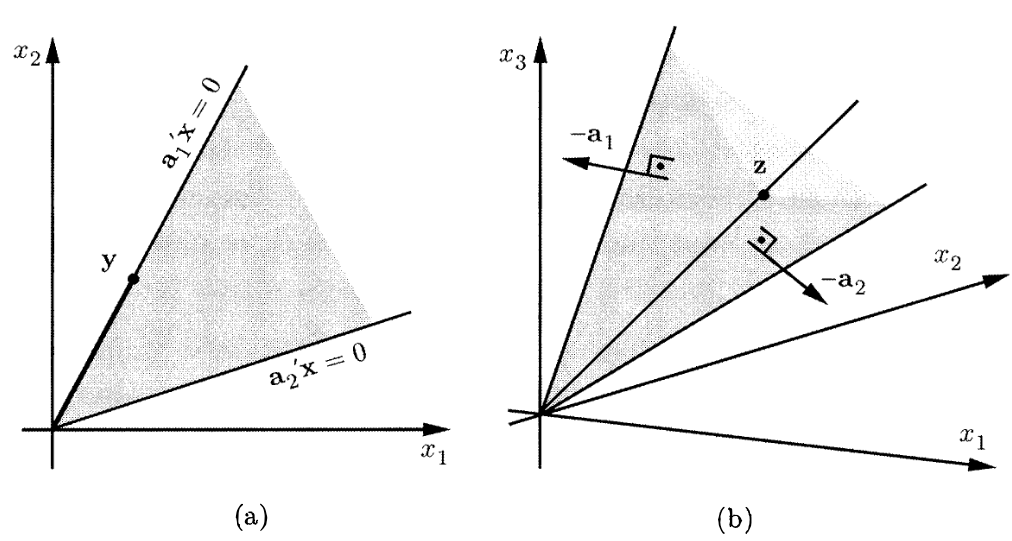
\includegraphics[width=0.5\linewidth]{figures/20261105214905217.png}
\end{center}


% Source Markdown lines 1284–1284
\begin{thmblock}[{Extreme rays on standard polyhedron}]
考虑优化问题 $\min_{\bm{x} \in \mathcal{C}} \bm{c}^\top \bm{x}$, 其中 $\mathcal{C} = \{\bm{x} \in \mathbb{R}^n: \bm{a}_i^\top \bm{x} \geq 0,~ i=1,\dots,m\}$ 是一个 pointed cone. 则最优值等于 $-\infty$ 当且仅当存在一个 extreme ray $\bm{d} \in \mathcal{C}$, 使得 $\bm{c}^\top \bm{d} < 0$.

\end{thmblock}


% Source Markdown lines 1286–1293
\begin{proof}{}
($\Leftarrow$) 若存在一个 extreme ray $\bm{d} \in \mathcal{C}$, 使得 $\bm{c}^\top \bm{d} < 0$, 则对于任意 $\lambda \geq 0$, 有 $\bm{x} + \lambda \bm{d} \in \mathcal{C}$, 且 $\bm{c}^\top (\bm{x} + \lambda \bm{d}) = \bm{c}^\top \bm{x} + \lambda \bm{c}^\top \bm{d}$, 随着 $\lambda \to +\infty$, $\bm{c}^\top (\bm{x} + \lambda \bm{d}) \to -\infty$, 故最优值为 $-\infty$.

($\Rightarrow$) 欲证: 若最优值为 $-\infty$, 则存在一个 extreme ray $\bm{d} \in \mathcal{C}$, 使得 $\bm{c}^\top \bm{d} < 0$.

\begin{itemize}
\item {}首先, 由于最优值为 $-\infty$, 故定存在 $\bm{x} \in \mathcal{C}$, 使得 $\bm{c}^\top \bm{x} < 0$. 对 $\bm{x}$ 费用进行归一化为 $\tilde{\bm{x}} = {\bm{x}}/{(-\bm{c}^\top \bm{x})}$, 则 $\tilde{\bm{x}} \in \mathcal{C}$ 且 $\bm{c}^\top \tilde{\bm{x}} = -1$. 方便起见, 这里仍将 $\tilde{\bm{x}}$ 记为 $\bm{x}$. 故现有集合 $\mathcal{P} = \{\bm{x}: \bm{a}_i^\top \bm{x} \geq 0,~ i=1,\dots,m,~ \bm{c}^\top \bm{x} = -1\}$ 是一个 polyhedron, 且 $\mathcal{P} \neq \varnothing$.


\item {}由于 $\mathcal{C}$ 是 pointed cone, 故 $\bm{a}_1, \dots, \bm{a}_m$ 可以张成 $\mathbb{R}^n$. 而 $\mathcal{P}$ 是在 $\mathcal{C}$ 的基础上增加了一个线性约束 $\bm{c}^\top \bm{x} = -1$, 其不会减少张成的空间维度. 回顾, 对于 polyhedron $\mathcal{P}$, 其存在极点 iff 其不包含完整直线 iff $\operatorname{span}\{\bm{a}_1, \dots, \bm{a}_m, \bm{c}\} = \mathbb{R}^n$. 故 $\mathcal{P}$ 至少有一个 extreme point, 记为 $\bm{d}$. 此时有 $\bm{c}^\top \bm{d} = -1 < 0$.


\item {}下证明 $\bm{d}$ 是 $\mathcal{C}$ 的extreme ray. 由于 $\bm{d} \in \mathcal{P}$, 其等式约束恒成立. 而又因为在 $\bm{d}$ 处有 $n$ 个线性无关的 active constraints, 故除去 $\bm{c}^\top \bm{d}=-1$ 这一约束后, $\bm{d}$ 处锥约束的秩恰为 $n-1$, 故 $\bm{d}$ 是 $\mathcal{C}$ 的 extreme ray.


\end{itemize}

\end{proof}


% Source Markdown lines 1295–1295
\begin{colblock}{}
上述论述还可以进一步推广到一般的 polyhedron $\mathcal{P} = \{\bm{x} \in \mathbb{R}^n: \bm{A}\bm{x} \geq \bm{b}\}$. 假设 $\mathcal{P}$ 至少有一个 extreme point, 则最优值为 $-\infty$ 当且仅当存在一个 extreme ray $\bm{d}$, 使得 $\bm{c}^\top \bm{d} < 0$.

\end{colblock}

\subsection{Representations of polyhedra}

对于多面体 Polyhedron, 可以有两种不同的表示方式.


% Source Markdown lines 1302–1310
\begin{defblock}[{H- and V-representations}]
\begin{itemize}
\item {}\emph{\textbf{H(alf-space) representation}}. H-representation 是在外部通过一系列超平面进行划分框定, 得到的多面体. 形如

\[
  \mathcal{P} = \{\bm{x}: \bm{A}\bm{x} \leq \bm{b}, \bm{C}\bm{x} = \bm{d}\}
\]


\item {}\emph{\textbf{V(ertices) representation}}. V-representation 是通过描述多面体的有限生成点, 用这些点的凸包来表示多面体. 此外通过引入 cone 来表示 unbounded 的部分. 形如

\[
  \mathcal{P} = \text{conv}(\mathcal{V}) + \text{cone}(\mathcal{R})
\]

其中, $\text{conv}(\mathcal{V})$ 表示有限生成点集 $\mathcal{V}$ 的凸包, $\text{cone}(\mathcal{R})$ 表示射线集合 $\mathcal{R}$ 的凸锥, 求和为 Minkowski sum. 即, 任意非空 pointed polyhedron 都可以表示为 extreme point 的凸组合 + extreme ray 的非负组合; 一般 polyhedron 的有限生成点和生成方向不必是极点与极射线.


\end{itemize}

\end{defblock}

可以证明, 这两种表示是等价的.


\end{document}
